% !TEX TS-program = latex
% IACR Transactions CLASS DOCUMENTATION -- version 0.24 (26 August 2016)
% Written by Gaetan Leurent gaetan.leurent@inria.fr (2016)
%
% To the extent possible under law, the author(s) have dedicated all
% copyright and related and neighboring rights to this software to the
% public domain worldwide. This software is distributed without any
% warranty.
%
% You should have received a copy of the CC0 Public Domain Dedication
% along with this software. If not, see
% <http://creativecommons.org/publicdomain/zero/1.0/>.

\documentclass[submission]{iacrtrans}
%\documentclass{iacrtrans}
\usepackage[utf8]{inputenc}
% *** MATH PACKAGES ***
%
\usepackage{amsmath}
\usepackage{listings}% use mathematical symbols in Verbatim environment
\lstset{
  basicstyle=\ttfamily,
  mathescape
}
\usepackage{amsfonts,amssymb}
\usepackage[linesnumbered,boxed,vlined]{algorithm2e}
% *** ALIGNMENT PACKAGES ***
%
\usepackage{array}
% *** PDF, URL AND HYPERLINK PACKAGES ***
%
\usepackage{url}



%personal defined packages
\usepackage{multirow,array}
% *** TABLE FOOTNOTE PACKAGES ***
\usepackage[bottom]{footmisc}
\usepackage{footnote}
\makeatletter
\def\@xfootnote[#1]{%
  \protected@xdef\@thefnmark{#1}%
  \@footnotemark\@footnotetext}
\makeatother
\usepackage{threeparttable}
\usepackage{diagbox}

\usepackage{caption}
\usepackage{subcaption}

\usepackage{placeins}

 %table dash line
\usepackage{arydshln}

\usepackage{morefloats}

\usepackage{fancyvrb}
\usepackage{xcolor}

% align center vertically in table
\newcolumntype{L}[1]{>{\raggedright\arraybackslash}m{#1}}
\newcolumntype{C}[1]{>{\centering\arraybackslash}m{#1}}
\newcolumntype{R}[1]{>{\raggedleft\arraybackslash}m{#1}}

\newcommand{\tabincell}[2]{\begin{tabular}{@{}#1@{}}#2\end{tabular}}

\theoremstyle{plain}
\newtheorem{thm}{Theorem}[section]
\newtheorem{lem}[thm]{Lemma}
\newtheorem{prop}[thm]{Proposition}
\newtheorem*{cor}{Corollary}

\usepackage{makecell}

\author[Jingwei Hu \textit{et. al.}]{Jingwei Hu\inst{1} \and Wen Wang\inst{2} \and Chaoping Xing\inst{3} \and San Ling\inst{1} \and Huaxiong Wang\inst{1}}
\institute{School of Physical and Mathematical Sciences, Nanyang Technological University, Singapore, \email{davidhu, lingsan, hxwang@ntu.edu.sg} \and Department of Electronic Engineering, Yale University, USA, \\\email{wen.wang.ww349@yale.edu} \and School of Cyberspace Security, Shanghai Jiaotong University, China, \\\email{xingcp@sjtu.edu.cn}}
\title[Memory Swapping based Number-Theoretic Transform for Fully Homomorphic Encryption]{Memory Swapping based Number-Theoretic Transform for Fully Homomorphic Encryption}
%\subtitle{\LaTeX{} Class Documentation (v. 0.24)}

\begin{document}

\maketitle

% use optional argument because the \LaTeX command breaks the PDF keywords
\keywords{Post-Quantum Cryptography, Rank Metric Code, Gaussian Elimination, FPGA Implementation}

\begin{abstract}
  In this paper, we investigate the practical performance of rank-code based cryptography on FPGA platforms by presenting a case study on a quantum-safe key encapsulation mechanism based on LRPC codes 
\end{abstract}

\section*{Introduction}
Post-quantum cryptogrpahy (PQC) refers to cryptographic public-key algorithms which exploit the hard problems thought to be outside bounded-error quantum polynomial time (BQP) class. As of 2021, most popular public-key algorithms rely on the BQP class problems and are theoretically insecure against an attack by a quantum computer. Even though it is not yet known to what extent a future quantum computer can be used to successfully solve BQP problems, many cryptographers are
designing new algorithms to prepare for a time when quantum computing becomes a real threat. This line of work has gained greater attention from academics and industry, including a European large project PQCRYPTO and a standardization competition initiated by NIST~\cite{chen2016report} in 2017. Currently, the PQC research is mostly focused on lattice-based, code-based, hash-based, isogeny-based, and multi-variate cryptography~\cite{bernstein2009introduction}.

\textit{Contributions.} This paper presents the first efficient and scalable FPGA-based cryptographic hardware for a post-quantum KEM/PKE using rank-metric codes (ROLLO). The main contributions include:
\begin{itemize}
\item a new, constant-time hardware design of Gaussian elimination for large-scaled (singular) matrices over binary field
\item a tunable, constant-time approach and design of polynomial multiplication over $\mathbb{F}_{2^m}[z]$
\item a more efficient, bounded decoding failure rate, and constant-time Rank Support Recovery (RSR) algorithm and its hardware implementation
\item a complete implementation of the ROLLO cryptosystem in support of various security parameters, which uses automatic code-generation scripts to generate vendor-neutral HDL codes
\end{itemize}


\section{FHEW-like Fully Homomorphic Encryption Scheme}
ROLLO is a compilation of two cryptographic schemes, \textit{i.e,} ROLLO-I and ROLLO-II which are among 26 round-2 candidates to the NIST's process for post-quantum cryptography standardization. ROLLO is based on rank metric codes and the difficult problem on which ROLLO relies is the syndrome decoding problem in the rank metric.
According to the most recent attacking preprint~\cite{bardet2020algebraic2}, the initial parameters used in ROLLO's round-2 submission are underestimated and later increased to reach its claimed security levels. In this paper, we stay focused on the latest parameters in the April-21-2020 version (see Table~\ref{table:security})~\cite{gaborit2017rollo}. It is also worth noting that ROLLO proposes 6 instances, each of which uses distinct system parameters. Therefore, it is challenging to realize the entire ROLLO on hardware which spans such a wide range of parameters. To tackle this challenge, the parameterization methodology is considered in this work such that the modules are fully parameterized and quickly switched from one parameter set to another for re-synthesis. We decide to use the parameter sets in the latest revised submission to showcase a dedicated hardware design for rank-code based cryptography and to better compare with the reference implementations in the ROLLO specification.

 

\section{Number-theoretic transform with merged twiddle factors}
This section describes ROLLO hardware at the bottom level. Firstly,  The distinguishing feature is that a series of new twiddle factor LUTs  is constructed and used:  an independent twiddle factor LUT, denoted as $\{w_i[\cdot]\}_{i=0,\ldots,log_2N-1}$, is prepared for the $i$-th round of butterfly computation ($logN$ rounds in total) as described in Alg.~\ref{alg:descript_twiddlefactor}.

\subsection{Higher level description for NTT with merged twiddle factors}\label{sec:gf2m_arith}

In this subsection, we discuss the NTT algorithm with merged twiddle factors. No pre-processing or post-processing is required in this variant of NTT algorithm. At an abstract level, the structure of this NTT algorithm is identical to that of the classic NTT algorithm. 


The formal description of this NTT variant is shown in Alg.~\ref{alg:descript_ntt}. It has $logN$ iterations (loop-$i$) at outermost, where each iteration computes one layer of butterfly computations.  The $i(i=0,\cdots,logN-1)$-th layer of butterfly computation always has $\frac{N}{2}$ butterflies. These butterfiles are bundled into $2^i$ groups (recorded by the variable $NumberofGroups$) and each groups has $\frac{N}{2^i}$ pairs of butterflies (recorded by the variable $PairsInGroup$). The key feature is that at a particular iteration (say the $i$-th iteration), the butterflies in a particular group (say the $k$-th group) share the same twiddle factor $w_i[k]$. The variable $Distance$ is used to locate precisely two inputs of a particular pair of butterfly in loop-$j$, \textit{i.e.}, $a[j]$ and $a[j+Distance]$.

A visualization of Alg.~\ref{alg:descript_ntt} is depicted in Fig.~\ref{fig:dit1} when $N=8$. The inputs are $a[0],\cdots,a[7]$. The NTT computation has 3 layers of butterfies: In the first layer ($i=0$ for loop-$i$ in Alg.), only one butterfly group (associated with twiddle factor $\omega_{16}^4$) exists; in the second layer, two butterfly groups (associated with twiddle factor $\omega_{16}^2$ and $\omega_{16}^6$) exist; in the third layer, four butterfly groups (associated with twiddle factors $\omega_{16}^1$, $\omega_{16}^5$, $\omega_{16}^3$, and $\omega_{16}^7$, respectively) exist. It is worth noting that the ouputs from the NTT network is in bit-reversed order as $A[0],A[4],A[2],A[6],A[1],A[5],A[3],A[7]$.

\begin{algorithm}[!tbh]
 \DontPrintSemicolon % Some LaTeX compilers require you to use \dontprintsemicolon instead
 \KwIn{polynomial $a(x)\in R_q$ represented in {}$a[\cdot]$, Twiddle factors $\{w_i[\cdot]\}_{i=0,\ldots,log_2N-1}$}
 \KwOut{NTT($a(x)$) represented in $a(x)$ (in-place)}
    $PairsInGroup \gets N/2$\;
    $NumOfGroups \gets 1$\;
    $Distance \gets N/2$\;
    \For{$i\leftarrow 0$ \KwTo $log_2N-1$}{
        \For{$k\leftarrow 0$ \KwTo $NumOfGroups-1$}{
            $JFirst \gets 2\cdot k \cdot PairsInGroup$\;
            $JLast \gets JFirst + PairsInGroup-1$\;
            \For{$j\leftarrow JFirst$ \KwTo $JLast$}{
                $Temp \gets w_i[k]*a[j+Distance]$\;
                $a[j+Distance] \gets a[j]-Temp$\;
                $a[j] \gets a[j] + Temp$\;
            }             
        }      
        $PairsInGroup \gets PairsInGroup/2$\;
        $NumOfGroups \gets NumOfGroups\cdot 2$\;
        $Distance \gets Distance/2$\;
    }
    \Return {$c(x)$\;}
 \caption{Higher level description of NTT}\label{alg:descript_ntt}
\end{algorithm}

\begin{algorithm}[!tbh]
 \DontPrintSemicolon % Some LaTeX compilers require you to use \dontprintsemicolon instead
 \KwIn{a polynomial ring $R_q$, and NTT points $N$}
 \KwOut{Twiddle factors $\{w_i[\cdot]\}_{i=0,\ldots,log_2N-1}$ used in Algorithm~\ref{alg:descript_ntt}}
    $FirstPart \gets [0\cdots0]_2$\;{}
    $SecondPart \gets [1\cdots0]_2$\;
    \For{$i\leftarrow 0$ \KwTo $log_2N-1$}{
        \For{$j\leftarrow 0$ \KwTo $N-1$}{
            $[j_{log_2N-1,\cdots,j_0}]_2 \gets BinRepr(j)$\;
            $w_i[j] \gets \phi^{Firstpart}\cdot \phi^{SecondPart}$\;         
        }   
        $FirstPart \gets RightRot(FirstPart, j_{log_2N-1-i})$\;   
        $SecondPart \gets SecondPart/2$\;
    }
    \Return {$\{w_i[\cdot]\}_{i=0,\ldots,log_2N-1}$\;}
 \caption{Construction of Twiddle Factor LUTs}\label{alg:descript_twiddlefactor}
\end{algorithm}

Next, we detail how to construct the twiddle factor LUT. Recall the NTT with pre-processing can be written together as a summation of $N$ terms:
\[
    A_i = \sum_{j=0}^{N-1}a_j\omega_{2N}^j\omega_N^{ij} \bmod q, i\in [0,N-1]
\]

Next, by splitting the summation above into even and odd groups according to the index $i$ of $A_i$, we obtain
\begin{gather}
    A_i = \sum_{j=0}^{\frac{N}{2}-1}a_{2j}\omega_N^{2ij}\omega_{2N}^{2j}  + \sum_{j=0}^{\frac{N}{2}-1}a_{2j+1}\omega_N^{i(2j+1)}\omega_{2N}^{2j+1} \bmod q \text{ for } i\in [0,\frac{N}{2}-1]\notag\\
    = \sum_{j=0}^{\frac{N}{2}-1}a_{2j}\omega_{\frac{N}{2}}^{ij}\omega_{N}^{j}  + \omega_{N}^i\omega_{2N}\sum_{j=0}^{\frac{N}{2}-1}a_{2j+1}\omega_{\frac{N}{2}}^{ij}\omega_N^{j} \bmod q \notag
\end{gather}
Now express $A_i$s into the first half $A_{i}$ and the second half $A_{i+\frac{N}{2}}$ as follows: 
\begin{gather}
    A_i = \sum_{j=0}^{\frac{N}{2}-1}a_{2j}\omega_{\frac{N}{2}}^{ij}\omega_{N}^{j}  + \omega_{N}^i\omega_{2N}\sum_{j=0}^{\frac{N}{2}-1}a_{2j+1}\omega_{\frac{N}{2}}^{ij}\omega_N^{j} \bmod q \text{ for } i\in [0,\frac{N}{2}-1]\notag\\
   A_{i+\frac{N}{2}} = \sum_{j=0}^{\frac{N}{2}-1}a_{2j}\omega_{\frac{N}{2}}^{ij}\omega_{N}^{j}  - \omega_{N}^i\omega_{2N}\sum_{j=0}^{\frac{N}{2}-1}a_{2j+1}\omega_{\frac{N}{2}}^{ij}\omega_N^{j} \bmod q \notag
\end{gather}

Assume $N=2^n$, let $Y_i^{(n-1)}$ and $Z_i^{(n-1)}$ be solutions to the two half-sized subproblems (NTT of size of $\frac{N}{2}$) defined by
\begin{gather}
    Y_i^{(n-1)} = \sum_{j=0}^{\frac{N}{2}-1}a_{2j}\omega_{\frac{N}{2}}^{ij}\omega_{N}^{j} \bmod q \text{ for } i\in [0,\frac{N}{2}-1]\notag\\
    Z_i^{(n-1)} = \sum_{j=0}^{\frac{N}{2}-1}a_{2j+1}\omega_{\frac{N}{2}}^{ij}\omega_N^{j} \bmod q \notag
\end{gather}

Therefore, the equation above is rewritten in a more compact form:
\begin{gather}
    Y_i^{(n)} = Y_i^{(n-1)} + \omega_{N}^i\omega_{2N}Z_i^{(n-1)} = A_i\bmod q \text{ for } i\in [0,\frac{N}{2}-1]\notag\\
    Z_i^{(n)} = Y_i^{(n-1)} - \omega_{N}^i\omega_{2N}Z_i^{(n-1)} = A_{i+\frac{N}{2}} \bmod q \notag
\end{gather}

The key observation for the equation above is that $Y_i^{(n)}$ and $Z_i^{(n)}$ has a recursive structure: for example, $Y_i^{(n)}$ and $Z_i^{(n)}$ are computed from a butterfly of  $Y_i^{(n-1)}$ and $Z_i^{(n-1)}$, $Y_i^{(n-1)}$ and $Z_i^{(n-1)}$ are computed from a butterfly of $Y_i^{(n-2)}$ and $Z_i^{(n-2)}$, and so on so forth. Note that in the $k$-th iteration of such recursion (\textit{i.e.}, $Y_i^{(k)}$ and $Z_i^{(k)}$, and let $K=2^k$), the twiddle factor always has the form $\omega_K^i\omega_{2K}$. As we have known from the standard FFT, the index $i$ in $\omega_K^i$ appears in bit-reversed order, therefore, we generalize the modified twiddle factor in our case as shown in Table~\ref{table:merged_tf}.
\begin{table}\centering
\begin{tabular}{lccccc}
 \hline
 NTT iteration $i$ & $i=0$ & $i=1$ & $\cdots$ & $i=n-2$ & $i=n-1$\\
 \hline
 \makecell{twiddle factor\\ associated with\\ $a[j]$ and\\ $a[j+distance]$} & $\omega_{N}^{\textcolor{red}{\overbrace{00\cdots00}^{n-1 \text{ bits}}}}\cdot \omega_{2N}^{\textcolor{red}{\overbrace{10\cdots00}^{n \text{ bits}}}}$ & $\omega_{N}^{\textcolor{red}{j_{n-1}0\cdots 00}}\cdot\omega_{2N}^{\textcolor{red}{01\cdots 00}}$  & $\cdots$ & $\omega_{N}^{\textcolor{red}{j_{2}j_{3}\cdots 00}}\cdot \omega_{2N}^{\textcolor{red}{00\cdots 10}}$ & $\omega_{N}^{\textcolor{red}{j_{1}j_{2}\cdots j_{n-2}j_{n-1}}}\cdot \omega_{2N}^{\textcolor{red}{00\cdots 01}}$\\
 \hline
 \end{tabular}
   \caption{Merged Twiddle Factor used in $N$-point NTT. The exponent is expressed in binary form.}
  \label{table:merged_tf}
 \end{table}

As shown in Table~\ref{table:merged_tf}, the updatd twidldle factor is composed of two multiplicative factors which is called the first part and the second part in this paper. The first part of the merged twiddle factor is identical to the standard NTT. We keep the same notations here and do not repeat the proof. It has the form $\omega_{N}^{\overbrace{00\cdots 00}^{n-1 \text{ bits}}}$, $\omega_{N}^{\overbrace{j_{n-1}0\cdots 00}^{n-1 \text{ bits}}}$, $\cdots$, $\omega_{N}^{\overbrace{j_1j_2\cdots j_{n-2}j_{n-1}}^{n-1 \text{ bits}}}$, for $i=0,1,\cdots,n-1$, respectively.
The second part of the merged twiddle factor is $\omega_{2N}^1$. However, the value of $N$ depends on the recursive structure of butterfly, for the $i$-th layer, the specific $N$, denoted as $N'=N/2^{n-1-i}$. In other words, the second part equals to $\omega_{2\cdot 2}^1, \omega_{2\cdot 4}^1$, $\cdots$, $\omega_{2N}^1$ for $i=0,1,\cdots,n-1$. Further to unify the notation, the second part is rewritten in binary form as $\omega_{2N}^{\overbrace{10\cdots 00}^{n\text{ bits}}}$, $\omega_{2N}^{\overbrace{01\cdots 00}^{n\text{ bits}}}$, $\cdots$, $\omega_{2N}^{\overbrace{00\cdots 01}^{n\text{ bits}}}$ for $i=0,1,\cdots,n-1$.

Alg.~\ref{alg:descript_twiddlefactor} formally describes how to construct the twiddle factors for each round of butterfly computation based on our first-part-second-part concept mentioned above.
The first impression on Alg.~\ref{alg:descript_twiddlefactor} might be that the size of twiddle factor LUTs is about $\mathcal{O}(NlogN)$: It has $logN$ rounds and each round cosumes $N/2$ twiddle factor for the $N/2$ pairs of input points.  The key observation for reducing the size of twiddle factor LUT $\{w_i[\cdot]\}_i$ is that many entries in $w_i[\cdot]$ are duplicates and thus redundant. In particular, $w_0[\cdot]$ has only one distinct element $w_0[0]$, $w_1[\cdot]$ has two distinct elements $w_1[0]$ and $w_1[N/2]$, $w_2[\cdots]$ has four distinct elements $w_2[0]$, $w_2[N/4]$, $w_2[2N/4]$, and $w_2[3N/4]$ and so on so forth. Therefore, the total valid entries used in $\{w_i[\cdot]\}$ equal to
\[
\sum_{i=0}^{log_2N-1} 2^i = N-1 = \mathcal{O}(N) 
\]

\begin{figure*}[!tb]
\centering
\begin{subfigure}[t]{0.85\textwidth}\centering
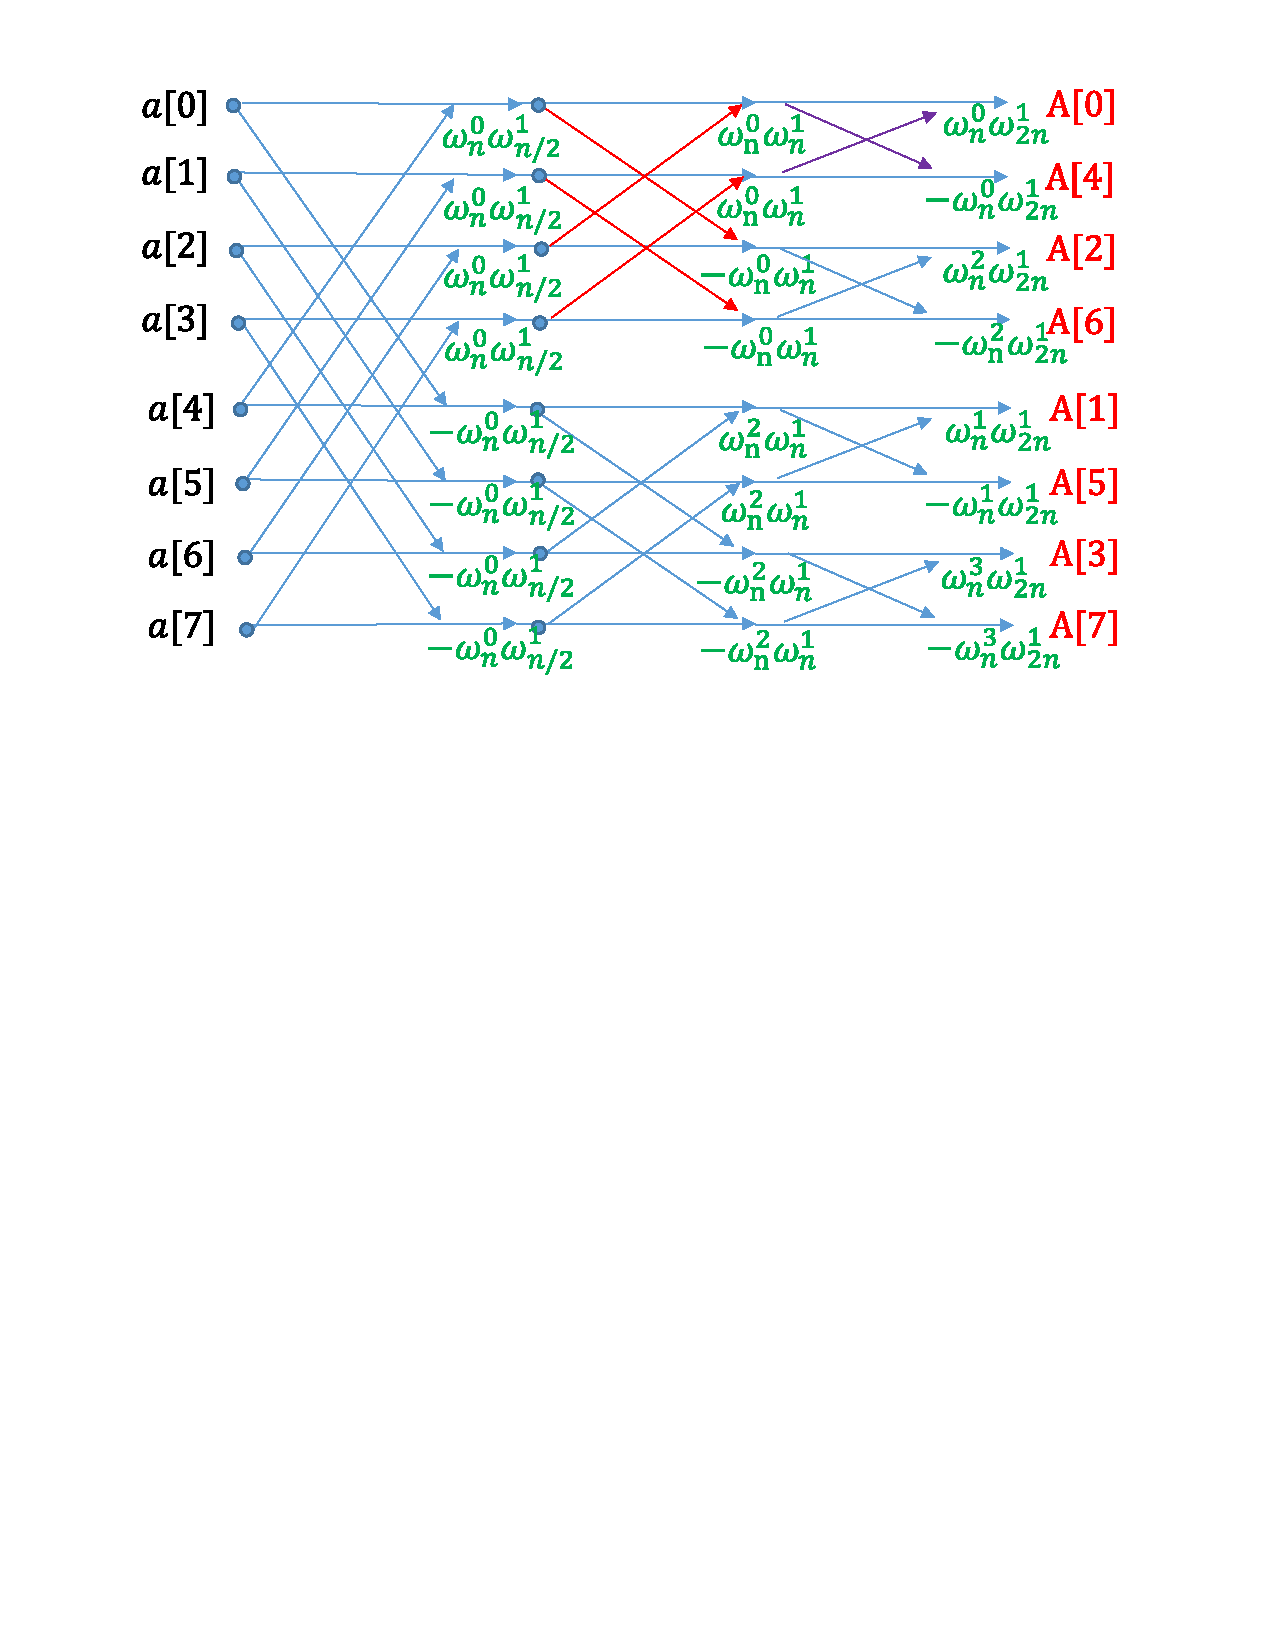
\includegraphics[width=\textwidth]{./fig/DIT1.pdf}
\caption{Generic architecture for NTT with merged twiddle factors ($N=8$)}
\label{fig:dit1}
\end{subfigure}

% \begin{subfigure}[t]{0.8\textwidth}\centering
% 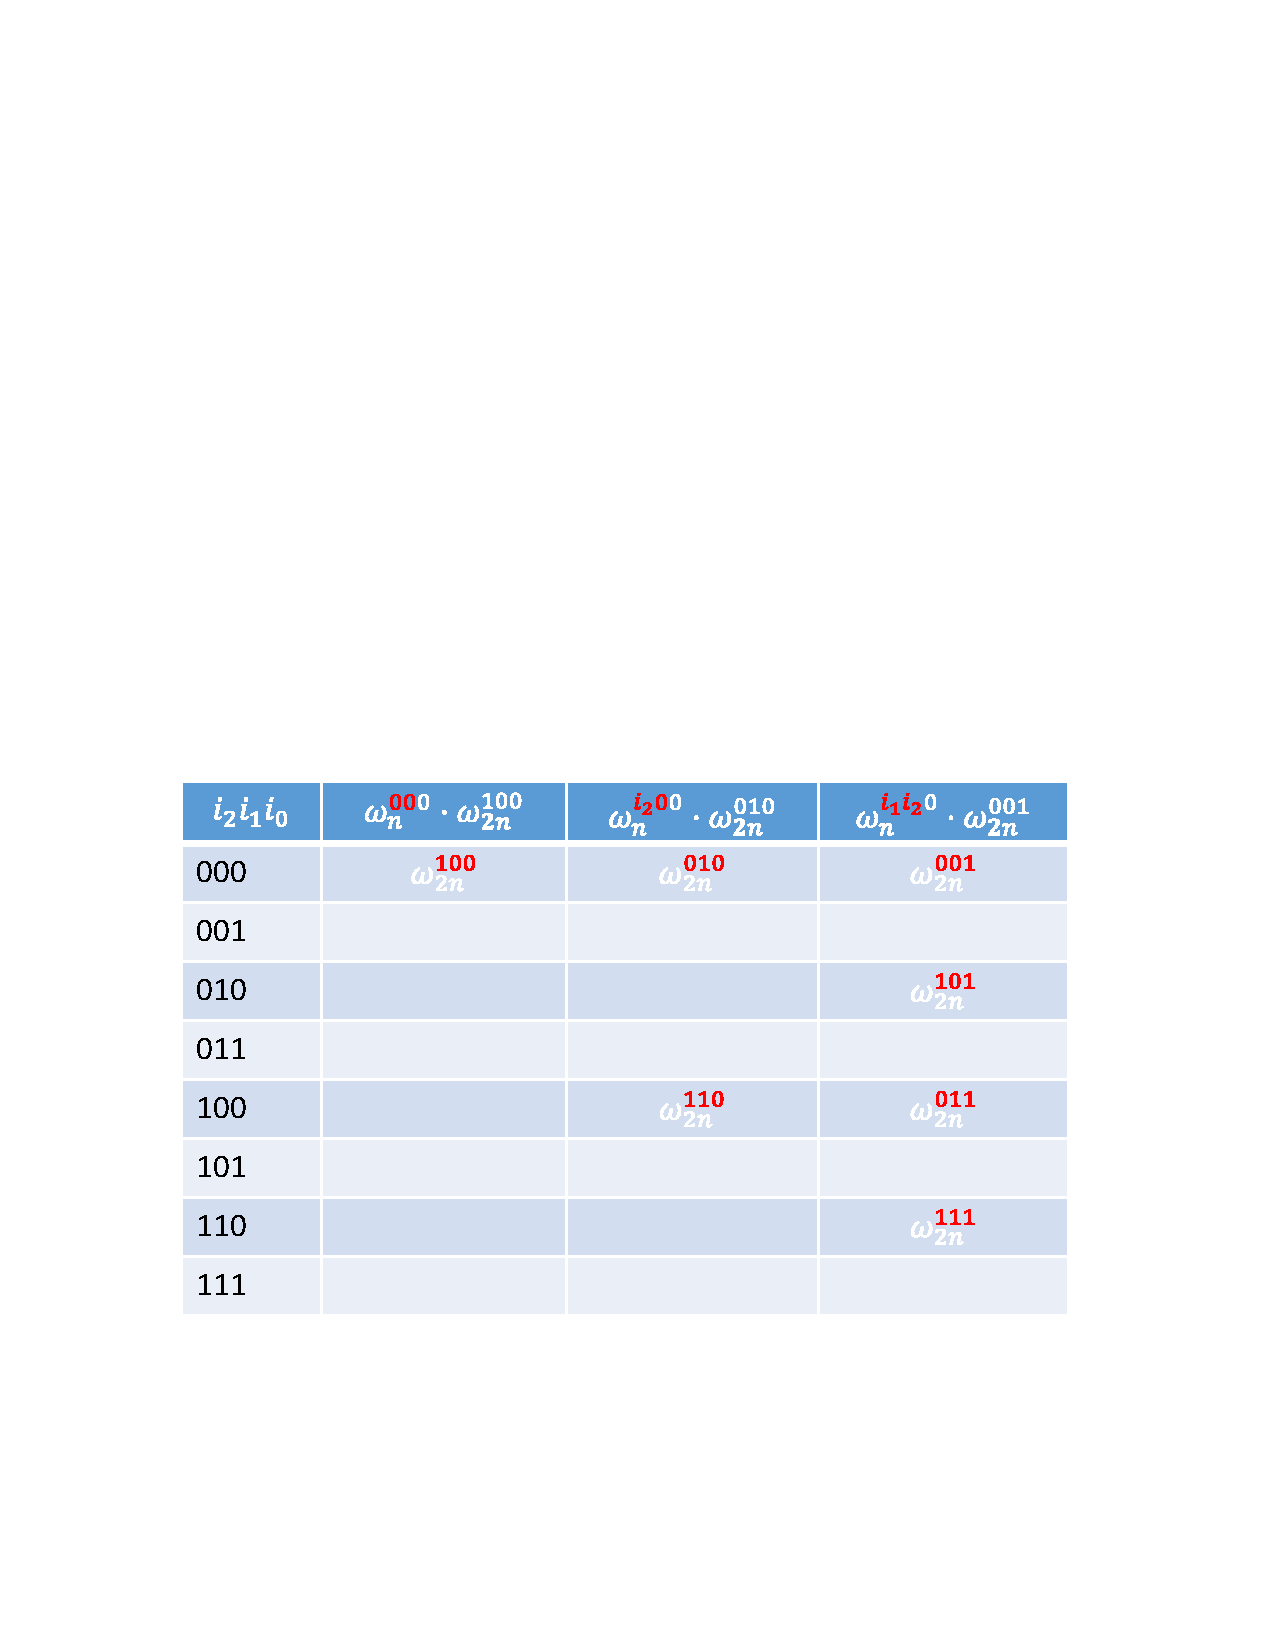
\includegraphics[width=\textwidth]{./fig/DIT2.pdf}
% \caption{Twiddle factor LUT context ($N=8$)}
% \label{fig:dit2}
% \end{subfigure}

\begin{subtable}[b]{0.8\textwidth}
  \centering
    \begin{tabular}{lccc}
     \hline
     $i=|i_2i_1i_0|_2$ & $\omega_N^{\textcolor{red}{00}}\cdot \omega_{2N}^{100}$ & $\omega_N^{\textcolor{red}{i_20}}\cdot \omega_{2N}^{010}$ & $\omega_N^{\textcolor{red}{i_1i_2}}\cdot \omega_{2N}^{001}$ \\
     \hline
     000 & \multirow{8}{*}{$\omega_{2N}^{\textcolor{red}{100}}$} & $\omega_{2N}^{\textcolor{red}{010}}$ & $\omega_{2N}^{\textcolor{red}{001}}$\\
     001 &                                      &                     &                     \\
     010 &                                      &                     & $\omega_{2N}^{\textcolor{red}{101}}$\\
     011 &                                      &                     &                     \\
     100 &                                      & $\omega_{2N}^{\textcolor{red}{110}}$ & $\omega_{2N}^{\textcolor{red}{011}}$\\
     101 &                                      &                     &                     \\
     110 &                                      &                     & $\omega_{2N}^{\textcolor{red}{111}}$\\
     111 &                                      &                     &                    \\
     \hline
     \end{tabular}
  \caption{Twiddle factor LUT context ($N=8$)}
  \label{table:table}
  \end{subtable}

\caption{DIT instance with $N=8$}
\end{figure*}


 % \begin{subtable}[!t]\centering
 % \caption{Twiddle factor LUT context ($N=8$)}
 % \label{table:gf2m-rollo-i}
 % \scalebox{1}{\begin{tabular}{lccc}
 % \hline
 % $i=|i_2i_1i_0|_2$ & $\omega_n^{\textcolor{red}{00}0}\cdot \omega_{2n}^{100}$ & $\omega_n^{\textcolor{red}{i_20}0}\cdot \omega_{2n}^{010}$ & $\omega_n^{\textcolor{red}{i_1i_2}0}\cdot \omega_{2n}^{001}$ \\
 % \hline
 % 000 & \multirow{8}{*}{$\omega_{2n}^{\textcolor{red}{100}}$} & $\omega_{2n}^{\textcolor{red}{010}}$ & $\omega_{2n}^{\textcolor{red}{001}}$\\
 % 001 &                                      &                     &                     \\
 % 010 &                                      &                     & $\omega_{2n}^{\textcolor{red}{101}}$\\
 % 011 &                                      &                     &                     \\
 % 100 &                                      & $\omega_{2n}^{\textcolor{red}{110}}$ & $\omega_{2n}^{\textcolor{red}{011}}$\\
 % 101 &                                      &                     &                     \\
 % 110 &                                      &                     & $\omega_{2n}^{\textcolor{red}{111}}$\\
 % 111 &                                      &                     &                    \\
 % \hline
 % \end{tabular}}
 % \end{subtable}


\subsection{$log_2d$-Dimensional Hypercube Multiprocessors}
\begin{figure*}[!tb]
\centering
\begin{subfigure}[t]{0.5\textwidth}\centering
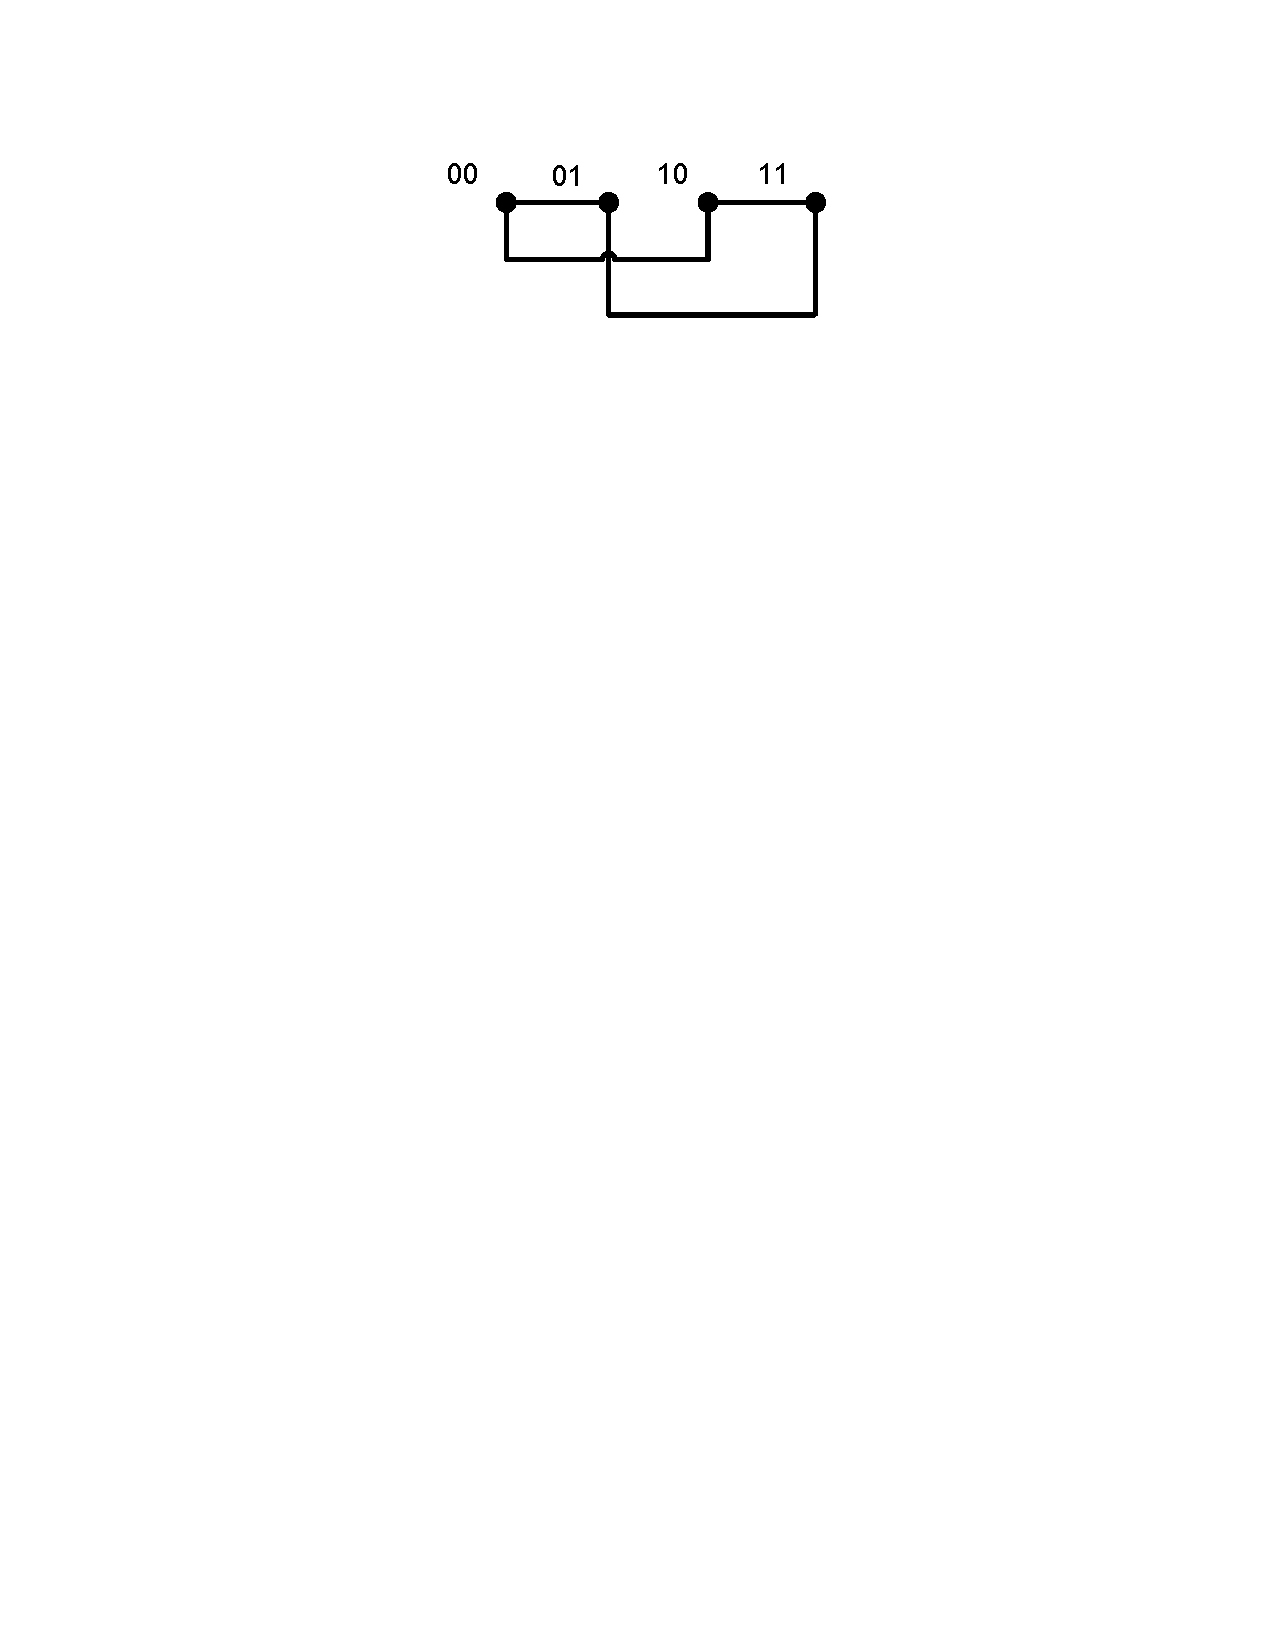
\includegraphics[width=\textwidth]{./fig/HyperCube1.pdf}
\caption{$d=4$, $ID\in\{P_0,P_1,P_2,P_3\}$}
\label{fig:dit1}
\end{subfigure}

\begin{subfigure}[t]{0.5\textwidth}\centering
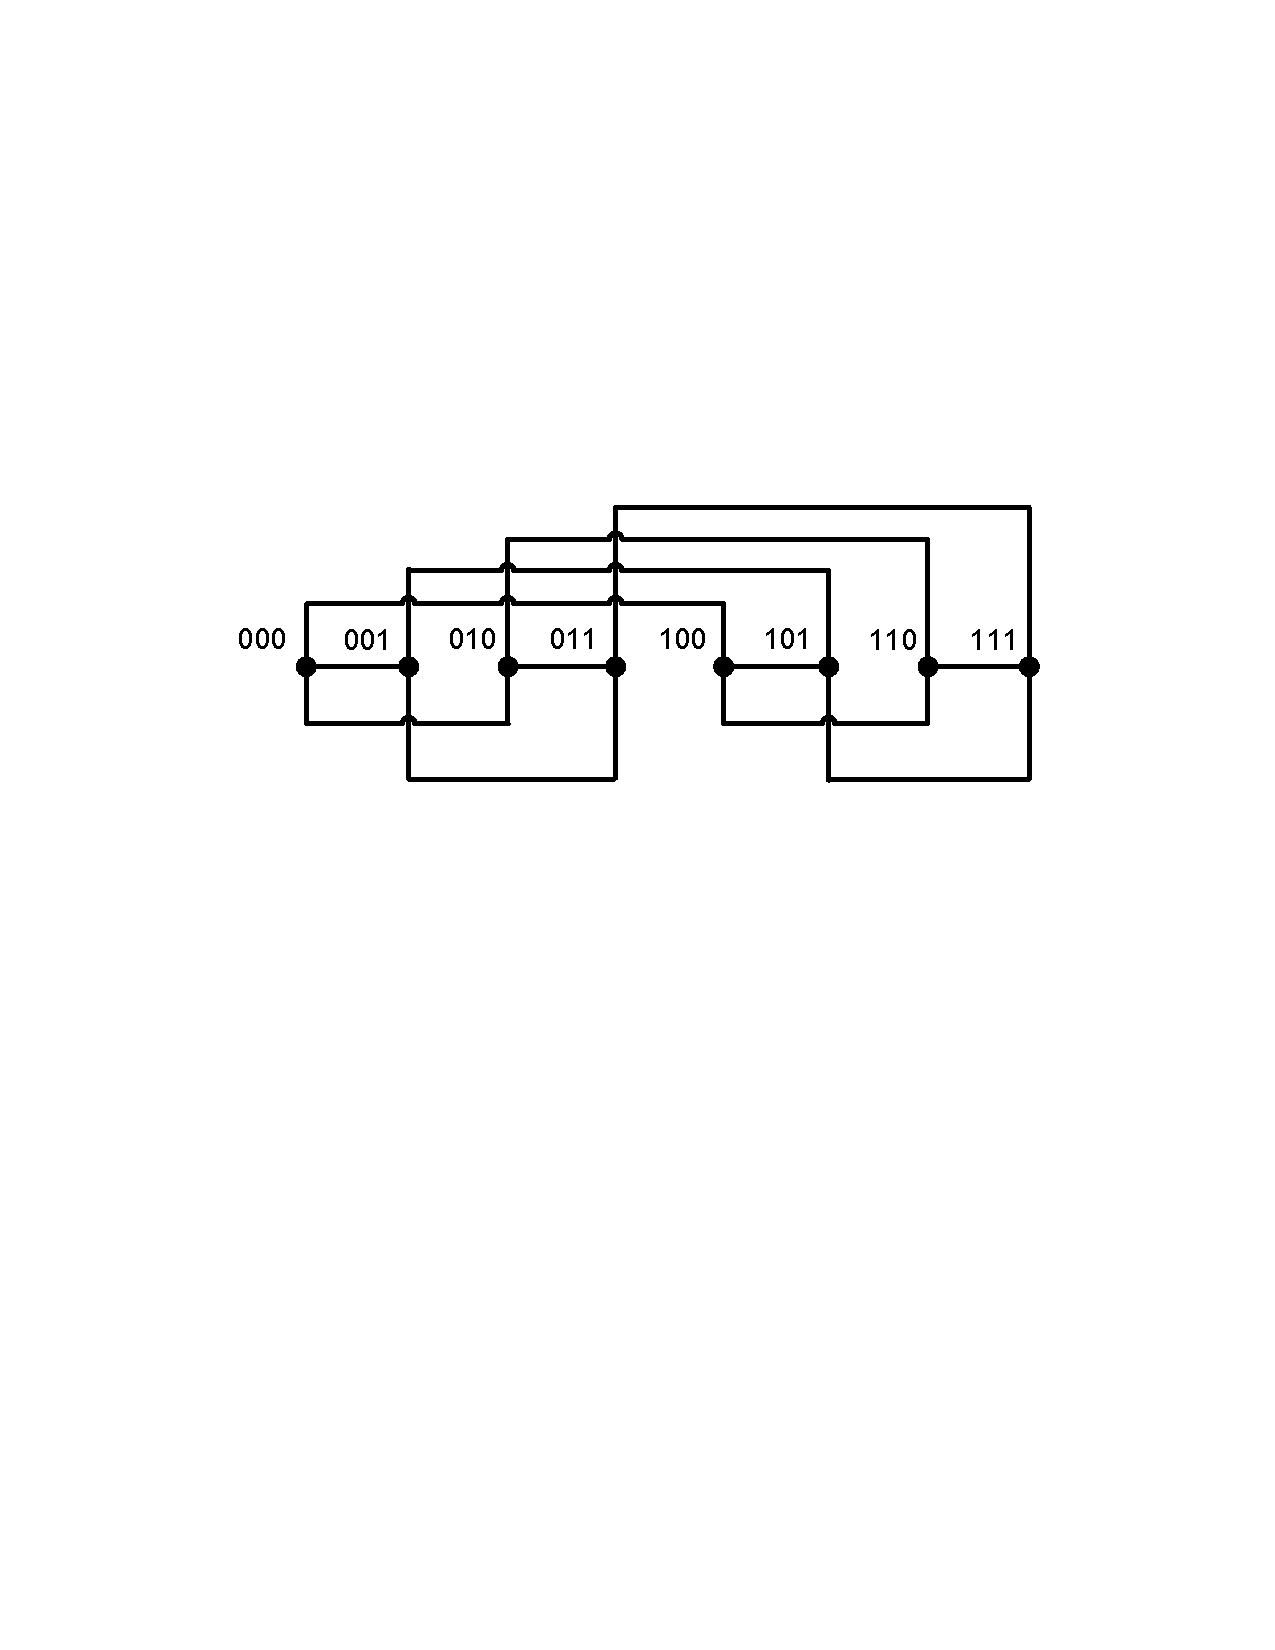
\includegraphics[width=\textwidth]{./fig/HyperCube2.pdf}
\caption{$d=8$, $ID\in\{P_0,P_1,P_2,P_3,P_4,P_5,P_6,P_7\}$}
\label{fig:dit2}
\end{subfigure}
\caption{Hypercubes of Dimension $log_2d=2,3$}
\end{figure*}

\begin{algorithm}[!tbh]
 \DontPrintSemicolon % Some LaTeX compilers require you to use \dontprintsemicolon instead
 \KwIn{$d$ node processors}
 \KwOut{$d$ node processors with connections}
    Denote the processor IDs as $\{P_0,P_1,\cdots,P_{d-1}\}$\;
    \For{$i\leftarrow 0$ \KwTo $d-1$}{  
        $[i_{log_2d-1,\cdots,i_0}]_2 \gets BinRepr(i)$\;     
        \For{$j\leftarrow 0$ \KwTo $log_2d-1$}{
            flip $i_j$ in $[i_{log_2d-1},\cdots,i_j,\cdots, i_0]_2$ to have $[i_{log_2d-1},\cdots,\bar{i_j},\cdots, i_0]_2$\;
            \uIf{$[i_{log_2d-1},\cdots,\bar{i_j},\cdots,i_0]_2 > [i_{log_2d-1},\cdots,i_j,\cdots,i_0]_2$}{
                  connect $P_{[i_{log_2d-1},\cdots,i_j,\cdots,i_0]_2}$ and $P_{[i_{log_2d-1},\cdots,\bar{i_j},\cdots,i_0]_2}$\;
                 }     
        }   
    }
    \Return {$c(x)$\;}
 \caption{Construction of the $log_2d$-dimensional hypercube}\label{alg:descript_hypercube}
\end{algorithm}

\begin{algorithm}[!tbh]
 \DontPrintSemicolon % Some LaTeX compilers require you to use \dontprintsemicolon instead
 \KwIn{$log_2d$-dimensional hypercubes}
 \KwOut{communication pattern}
    Denote the processor IDs as $\{P_0,P_1,\cdots,P_{d-1}\}$\;
    \For{$k\leftarrow 0$ \KwTo $log_2d-1$}{  
        /*$d/2$ pairs of processors exchange data in step-$k$*/\;
        exchange data between processors $P_{[i_{log2d-1},\cdots,i_{log_2d-1-k},\cdots,0]_2}$ and $P_{[i_{log2d-1},\cdots,\overline{i_{log_2d-1-k}},\cdots,0]_2}$ which differ at $i_{log_2d-1-k}$\;        
    }   
    \Return {$c(x)$\;}
 \caption{Subcube-doubling communication in $log_2d$-dimensional hypercube}\label{alg:descript_subcube}
\end{algorithm}

\begin{table}[h!]\begin{center}
 \caption{Subcube-doubling communication in $3$-dimensional hypercube}\label{tab:descript_subcube}
\begin{tabular}{l c}
\hline
  steps & connections\\
\hline
  Step-(0) & \raisebox{-0.5\height}{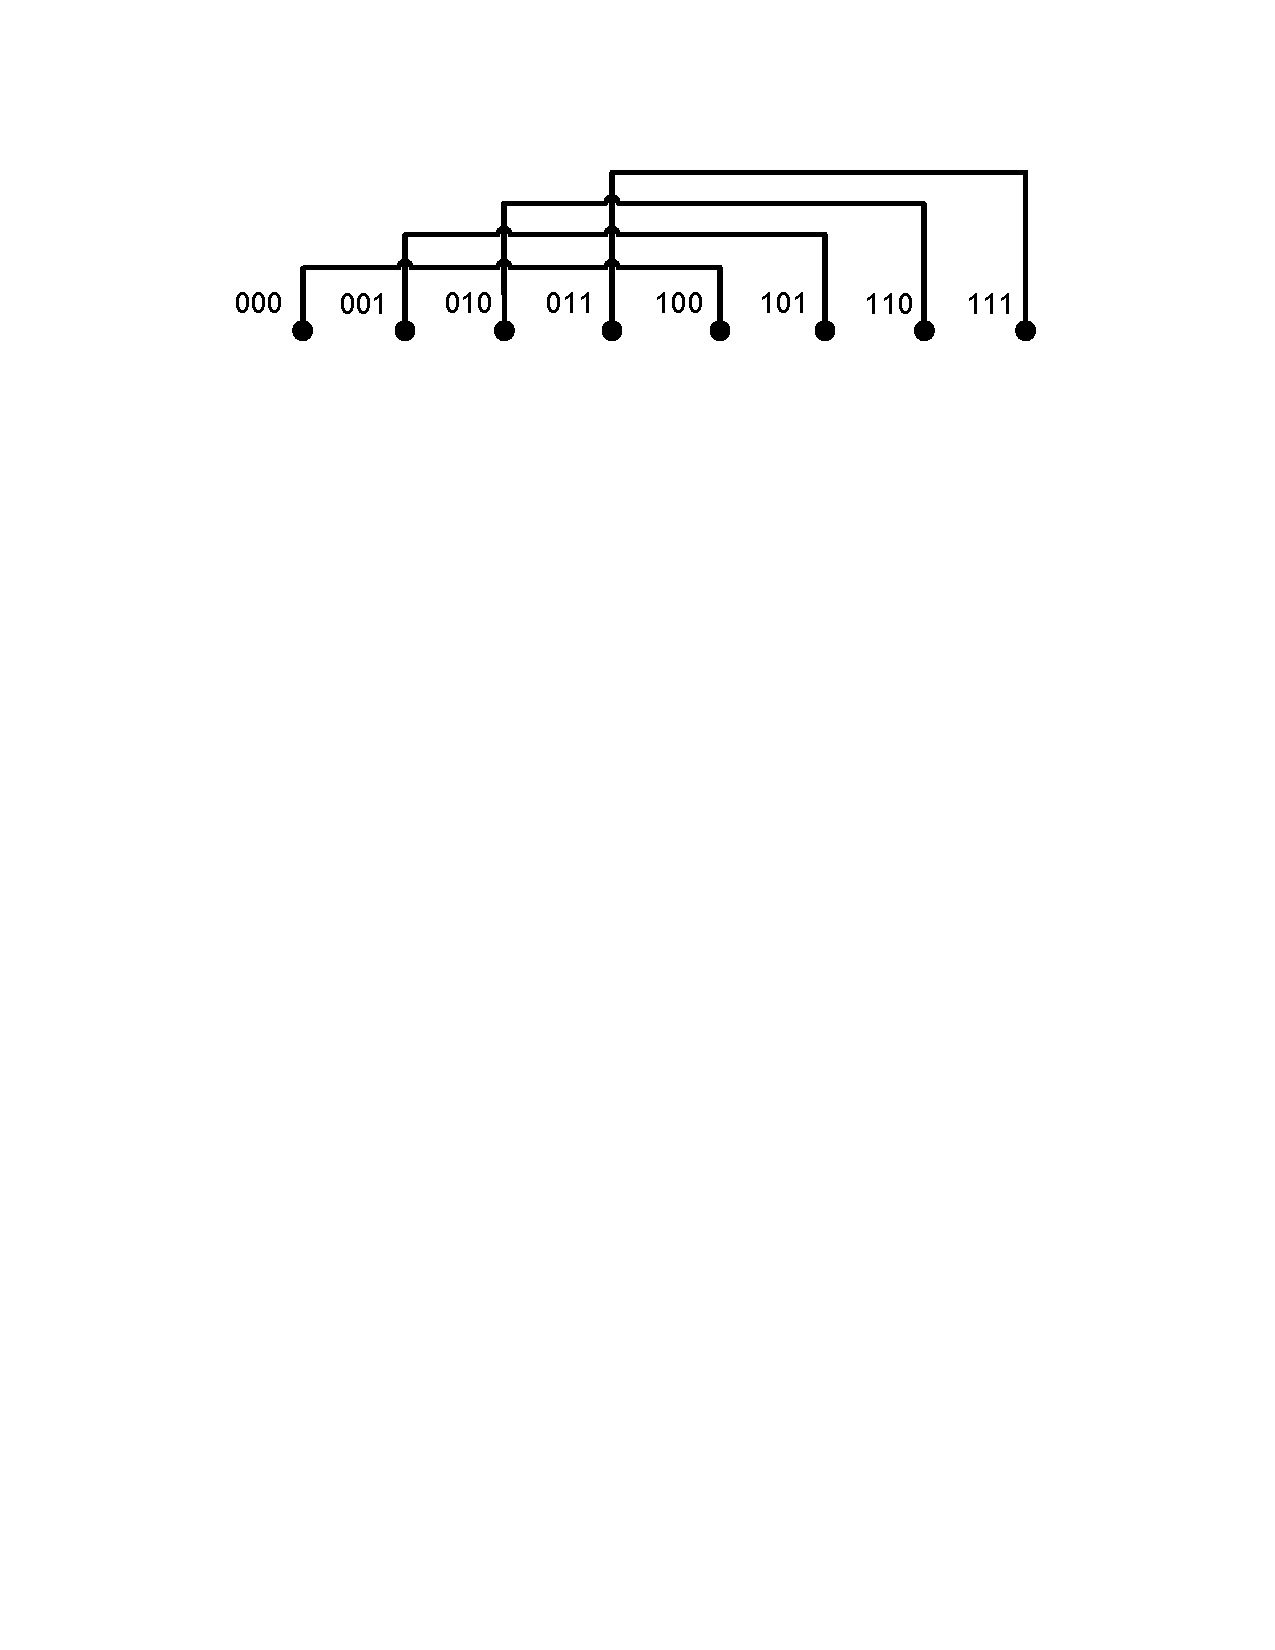
\includegraphics[width=.6\textwidth]{./fig/subcube_comm1.pdf}}\\
  Step-(1) & \raisebox{-0.5\height}{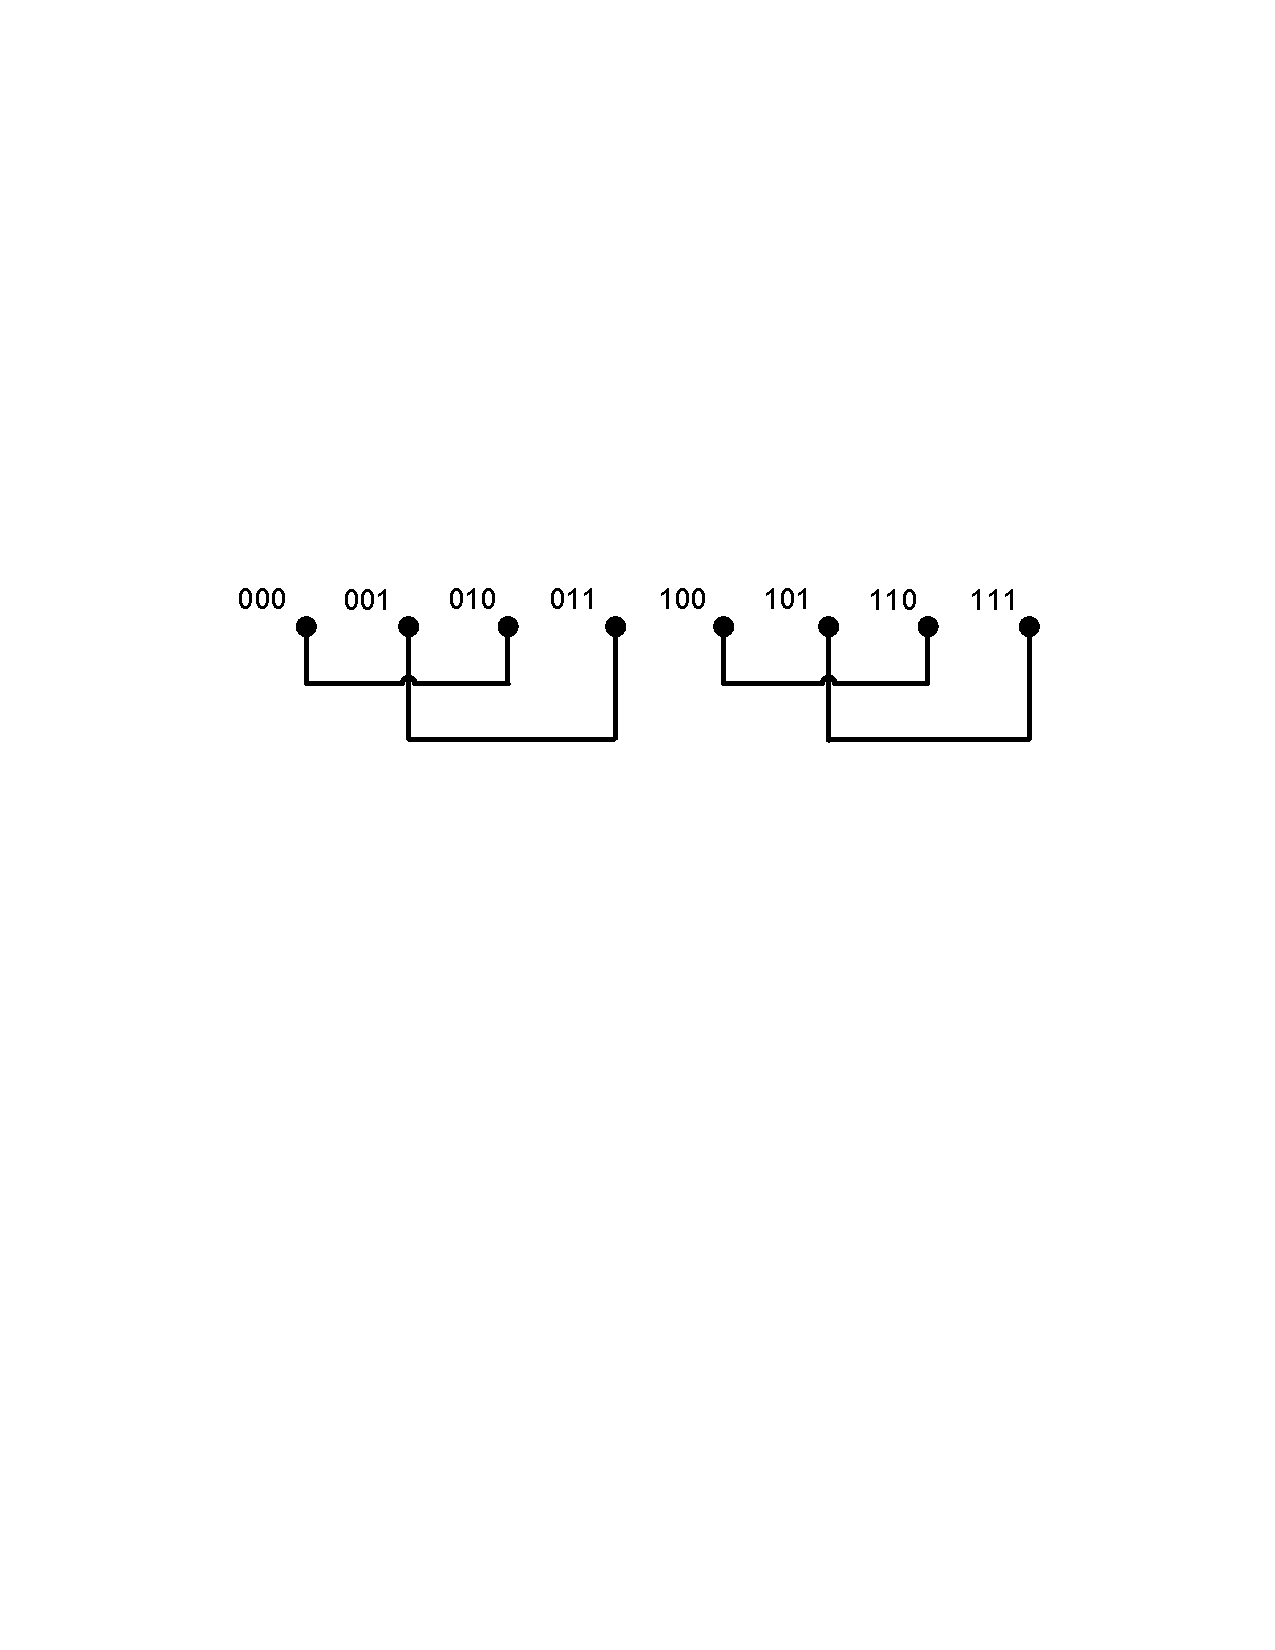
\includegraphics[width=.6\textwidth]{./fig/subcube_comm2.pdf}}\\
  Step-(2) & \raisebox{-0.5\height}{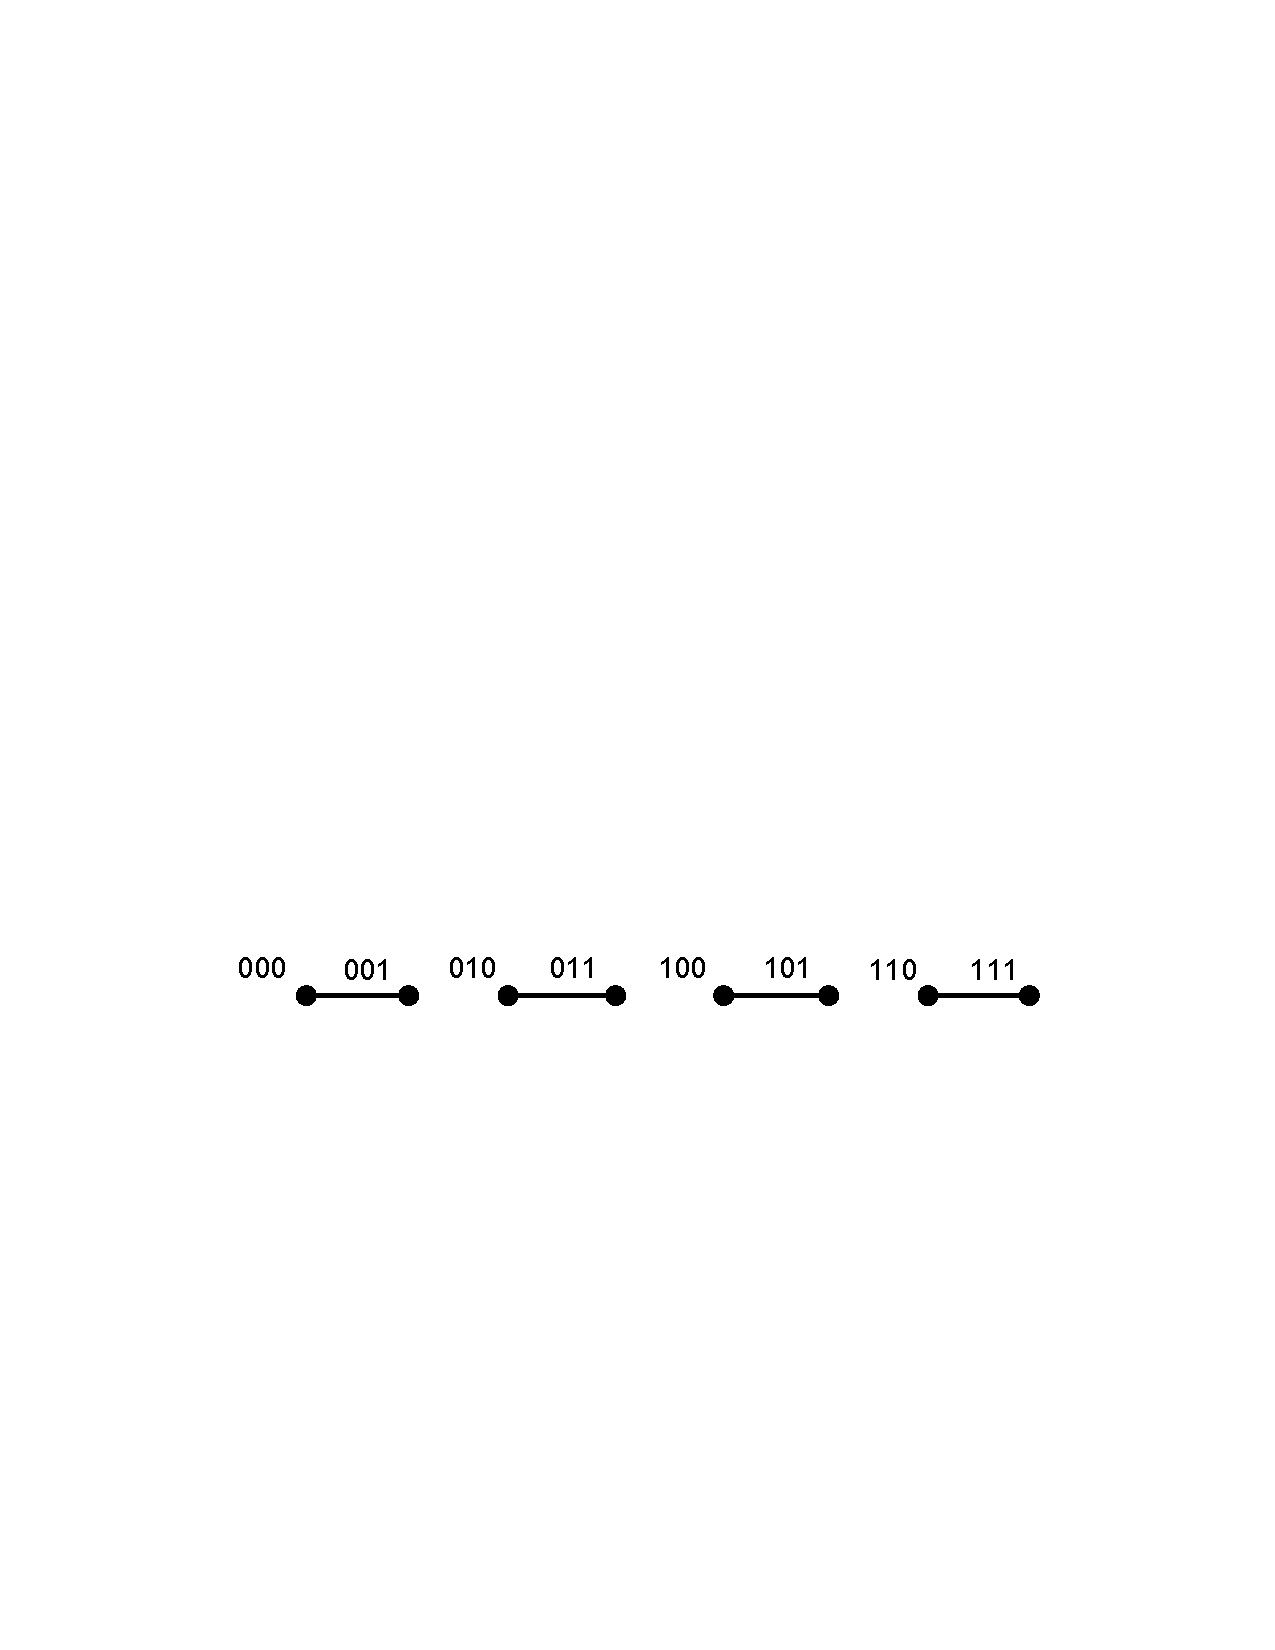
\includegraphics[width=.6\textwidth]{./fig/subcube_comm3.pdf}}\\
\hline  
\end{tabular}\end{center}  
\end{table}

In this subsection, we introduce the hypercube topology which fits the parallel NTT algorithm.

Before detailing the NTT algorithm and hardware, the computing model used in this paper must be clarified. There are $d$ identical node processors organized in a hypercube of dimension $log_2d$. Each node processor includes one butterfly unit and some storage ($N/d$ NTT points). Roughly speaking, this $log_2d$-dimensional hypercube structure should increase the speed of sequential NTT algorithm by $d$ times. 

Alg.~\ref{alg:descript_hypercube} describes how to construct the $log_2d$-dimensional hypercube by connecting $d$ node processors. The key idea here is that for each processor $P_i$, rewrite the index $i$ in binary form as $[i_{log_2d-1},\cdots,i_0]_2$, and connects those processors $P_j$ whose index $j=[j_{log_2d-1},\cdots,j_0]_2$ differs only 1 bit compared with $i$. In particular, each node processor connects only to $log_2d$ other node processors in this $log_2d$-dimensional hypercube topology.
{}
When the computation continues in the hypercube, the intermediate data generated in computation steps typically requires exchange between node processors. This type of data exchange is referred to as `subcube-doubling' communication in the literature. There are in total $log_2d$ rounds of exchange during the communication as described in Alg.~\ref{alg:descript_subcube}: In round-($k$), for each node processor $P_i$ with index $i=[i_{log_2d-1},\cdots,i_{0}]_2$. it exchanges data with $P_j$ whose index $j$ differs at the $log_2d-1-k$-th bit. 

An illustration instance with $d=8$ for subcube-doubling algorithm (Alg.~\ref{alg:descript_subcube}) is given in Table~\ref{tab:descript_subcube}. $log_2d=3$ communication steps are required in this example: In step-(0), processor $P_{[i_{2},i_{1},i_{0}]_2}$ connects processor $P_{[\overline{i_{2}},i_{1},i_{0}]_2}$ which differs at $i_{2}$, and there are $d/2=4$ such pairs of connections; In step-(1), processor $P_{[i_{2},i_{1},i_{0}]_2}$ connects processor $P_{[i_{2},\overline{i_{1}},i_{0}]_2}$ which differs at $i_{1}$; Finally, in step-(2), processor $P_{[i_{2},i_{1},i_{0}]_2}$ connects processor $P_{[i_{2},i_{1},\overline{i_{0}}]_2}$ which differs at $i_{0}$.


\subsection{A Useful Equivalent Notation: |PID|Local $M$}
Assume that $N$ points are stored in the global array $\mathbf{a}=\{a_{N-1},\cdots,0\}$ or simplified as $\mathbf{a}=\{a_i\}_{i=N-1,\cdots,0}$, and the elements in the array are assigned evenly to $d$ node processors. Then the array address based notation
\[
  i_{logN-1}\cdots i_{k+1}|i_k\cdots i_{k-logd+1}|i_{k-logd}\cdots i_0
\]
is used to denote that cosecutive $logd$ bits $i_k\cdots i_{k-logd+1}$ are chosen to specify the data-to-processor allocation.

In general, since any $logd$ bits can be used to form the processor ID number, it is easier to concatenate the bits representing the ID into one group denoted by `PID', and refers to the remaining $logN-logd$ bits, which are concatenated to form the local array address, as `Local $M$'. One can use the following equivalent notation, where the leading $d$ bits are always used to identify the processor ID number.
\[
  |\text{PID}|\text{Local } M = |\underbrace{i_k\cdots i_{k-logd+1}}_{logd}|\overbrace{i_{N-1}\cdots i_{k+2}i_{k+1}}^{N-k-1}\overbrace{i_{k-d}\cdots i_1i_0}^{k-logd+1}
\]
For example, suppose $N=32$ and the mapping is denoted by $i_0i_1$|$i_2i_3i_4$. To locate $a_m=a_{26}$, one writes down $m=26=11010_2=i_4i_3i_2i_1i_0$, from which one knows that $a_{26}$ is stored in $a[r]$, $r=i_0i_1i_2i_3i_4=01011_2=11$, and that $a[11]=a_{26}$ is located in processor $P_{i_0i_1}=P_{01}$.

Table~\ref{tab:pid_notation2} shows the local data of each processor after a naturally ordered input series of $N=32$ elements is divided among $d=4$ processors using one particular cyclic block mapping.

\begin{table}[h!]\begin{center}
 \caption{Local data in processor $P_{i_4i_3}$ expressed in terms of global array element $a[m],m=i_4i_3i_2i_1i_0$ for the notation $i_4i_3$|$i_2i_1i_0$}\label{tab:pid_notation2}
\scalebox{0.8}{\begin{tabular}{c c | c c | c c | c c}
\hline
  \tabincell{c}{|PID|Local $M$\\$i_4i_3$|$i_2i_1i_0$} & \tabincell{c}{$P_{i_4i_3}=P_{00}$\\$a[m]$} & \tabincell{c}{|PID|Local $M$\\$i_4i_3$|$i_2i_1i_0$} & \tabincell{c}{$P_{i_4i_3}=P_{01}$\\$a[m]$} &\tabincell{c}{|PID|Local $M$\\$i_4i_3$|$i_2i_1i_0$} & \tabincell{c}{$P_{i_4i_3}=P_{10}$\\$a[m]$} & \tabincell{c}{|PID|Local $M$\\$i_4i_3$|$i_2i_1i_0$} & \tabincell{c}{$P_{i_4i_3}=P_{11}$\\$a[m]$}\\
\hline
$00$|$000$ & $a[0]$ & $01$|$000$ & $a[8]$ & $10$|$000$ & $a[16]$ & $11$|$000$ & $a[24]$\\
$00$|$001$ & $a[1]$ & $01$|$000$ & $a[9]$ & $10$|$000$ & $a[17]$ & $11$|$000$ & $a[25]$\\
$00$|$010$ & $a[2]$ & $01$|$000$ & $a[10]$ & $10$|$000$ & $a[18]$ & $11$|$000$ & $a[26]$\\
$00$|$011$ & $a[3]$ & $01$|$000$ & $a[11]$ & $10$|$000$ & $a[19]$ & $11$|$000$ & $a[27]$\\
$00$|$100$ & $a[4]$ & $01$|$000$ & $a[12]$ & $10$|$000$ & $a[20]$ & $11$|$000$ & $a[28]$\\
$00$|$101$ & $a[5]$ & $01$|$000$ & $a[13]$ & $10$|$000$ & $a[21]$ & $11$|$000$ & $a[29]$\\
$00$|$110$ & $a[6]$ & $01$|$000$ & $a[14]$ & $10$|$000$ & $a[22]$ & $11$|$000$ & $a[30]$\\
$00$|$111$ & $a[7]$ & $01$|$000$ & $a[15]$ & $10$|$000$ & $a[23]$ & $11$|$000$ & $a[31]$\\
\hline  
\end{tabular}}
\end{center}\end{table}

On the other hand, when the input elements are stored in $\mathbf{a}$ in bit-reversed order, \textit{i.e.,} $a[r]=a_m$ where $m=i_{n-1}i_{n-2}\cdots i_{0}$, and $r=i_0\cdots i_{n-2}i_{n-1}$, then the equivalent notation is as follows:
\[
  |\text{PID}|\text{Local } M = |\underbrace{i_{k-logd+1}\cdots i_{k}}_{logd}|\overbrace{i_{0}\cdots i_{k-logd}}^{k-logd+1}\overbrace{i_{k+1}\cdots i_{n-1}}^{N-k-1}
\]

\begin{table}[h!]\begin{center}
 \caption{Local data in processor $P_{i_0i_1}$ (bit reversed) expressed in terms of global array element $a[r]=a_m,r=i_0i_1i_2i_3i_4,m=i_4i_3i_2i_1i_0$ for the notation $i_0i_1$|$i_2i_3i_4$}\label{tab:pid_notation}
\scalebox{0.8}{\begin{tabular}{c c | c c | c c | c c}
\hline
  \tabincell{c}{|PID|Local $M$\\$i_0i_1$|$i_2i_3i_4$} & \tabincell{c}{$P_{i_0i_1}=P_{00}$\\$a[r]$} & \tabincell{c}{|PID|Local $M$\\$i_0i_1$|$i_2i_3i_4$} & \tabincell{c}{$P_{i_0i_1}=P_{01}$\\$a[r]$} &\tabincell{c}{|PID|Local $M$\\$i_0i_1$|$i_2i_3i_4$} & \tabincell{c}{$P_{i_0i_1}=P_{10}$\\$a[r]$} & \tabincell{c}{|PID|Local $M$\\$i_0i_1$|$i_2i_3i_4$} & \tabincell{c}{$P_{i_0i_1}=P_{11}$\\$a[r]$}\\
\hline
$00$|$000$ & $a[0]$ & $01$|$000$ & $a[8]$ & $10$|$000$ & $a[16]$ & $11$|$000$ & $a[24]$\\
$00$|$001$ & $a[1]$ & $01$|$000$ & $a[9]$ & $10$|$000$ & $a[17]$ & $11$|$000$ & $a[25]$\\
$00$|$010$ & $a[2]$ & $01$|$000$ & $a[10]$ & $10$|$000$ & $a[18]$ & $11$|$000$ & $a[26]$\\
$00$|$011$ & $a[3]$ & $01$|$000$ & $a[11]$ & $10$|$000$ & $a[19]$ & $11$|$000$ & $a[27]$\\
$00$|$100$ & $a[4]$ & $01$|$000$ & $a[12]$ & $10$|$000$ & $a[20]$ & $11$|$000$ & $a[28]$\\
$00$|$101$ & $a[5]$ & $01$|$000$ & $a[13]$ & $10$|$000$ & $a[21]$ & $11$|$000$ & $a[29]$\\
$00$|$110$ & $a[6]$ & $01$|$000$ & $a[14]$ & $10$|$000$ & $a[22]$ & $11$|$000$ & $a[30]$\\
$00$|$111$ & $a[7]$ & $01$|$000$ & $a[15]$ & $10$|$000$ & $a[23]$ & $11$|$000$ & $a[31]$\\
\hline  
\end{tabular}}
\end{center}\end{table}


\subsection{First attempt: parallel in-place FFTs without inter-processor permutations}

Consider the $DIT_{NR}$ algorithm and use the cyclic block mapping introduced in the last subsection. For $N=32$, the computation is depicted below:

\begin{table}[h!]\begin{center}
\scalebox{0.8}{\begin{tabular}{c c c c c c}
\hline
$|i_4i_3|i_2i_1i_0$ & $|\overset{\blacktriangledown}{\underset{\triangle}{i_4}}i_3|i_2i_1i_0$ & $|\tau_4\overset{\blacktriangledown}{\underset{\triangle}{i_3}}|i_2i_1i_0$ & $|\tau_4\tau_3|\overset{\blacktriangledown}{i_2}i_1i_0$ & $|\tau_4\tau_3|\tau_2\overset{\blacktriangledown}{i_1}i_0$ & $|\tau_4\tau_3|\tau_2\tau_1\overset{\blacktriangledown}{i_0}$\\
Initial Map   &   $\Longleftarrow\Longrightarrow$ &  $\Longleftarrow\Longrightarrow$ \\
\hline
\end{tabular}}
\end{center}\end{table}

The shorthand notation previously used for sequential NTT is augmented by two additional symbols. The double-headed arrow $\Longleftarrow\Longrightarrow$ indicates that $\frac{N}{d}$ data elements must be exchanged between processors in advance of butterfly computation. The symbol $i_k$ identifies two things:
\begin{itemize}
  \item First, it indicates the input source of external data: the incoming data from another processor are the elements whose addresses differ from a processor's own data in bit $i_k$.
  \item Second, it indicates that all pairs of processors whose binary ID number differ in bit $i_k$ send each other a copy of their own data.
\end{itemize}

The required data communications before the first stage of butterfly computation are explicitly depicted in Fig.~\ref{fig:dataswap_without_perm1} and Fig.~\ref{fig:dataswap_without_perm2}:  $P_0$ swaps data with $P_2$ such that $a[i]$ pairs with $a[i+16]$ to perform the required butterfly computation in the same processor for $i=0,\cdots,7$, and $P_1$ swaps data with $P_3$ such that $a[i]$ pairs with $a[i+16]$ to perform the required butterfly computation in the same processor for $i=8,\cdots,15$; the required data communications before the second stage of butterfly computation are depicted in Fig.~\ref{fig:dataswap_without_perm3} and Fig.~\ref{fig:dataswap_without_perm4}: $P_0$ swaps data with $P_1$ such that $a[i]$ pairs with $a[i+8]$ to perform the required butterfly computation in the same processor for $i=0,\cdots,7$, and $P_2$ swaps data with $P_3$ such that $a[i]$ pairs with $a[i+8]$ to perform the required butterfly computation in the same processor for $i=16,\cdots,23$.

\begin{figure*}[!tb]
\centering
\begin{subfigure}[b]{0.47\textwidth}
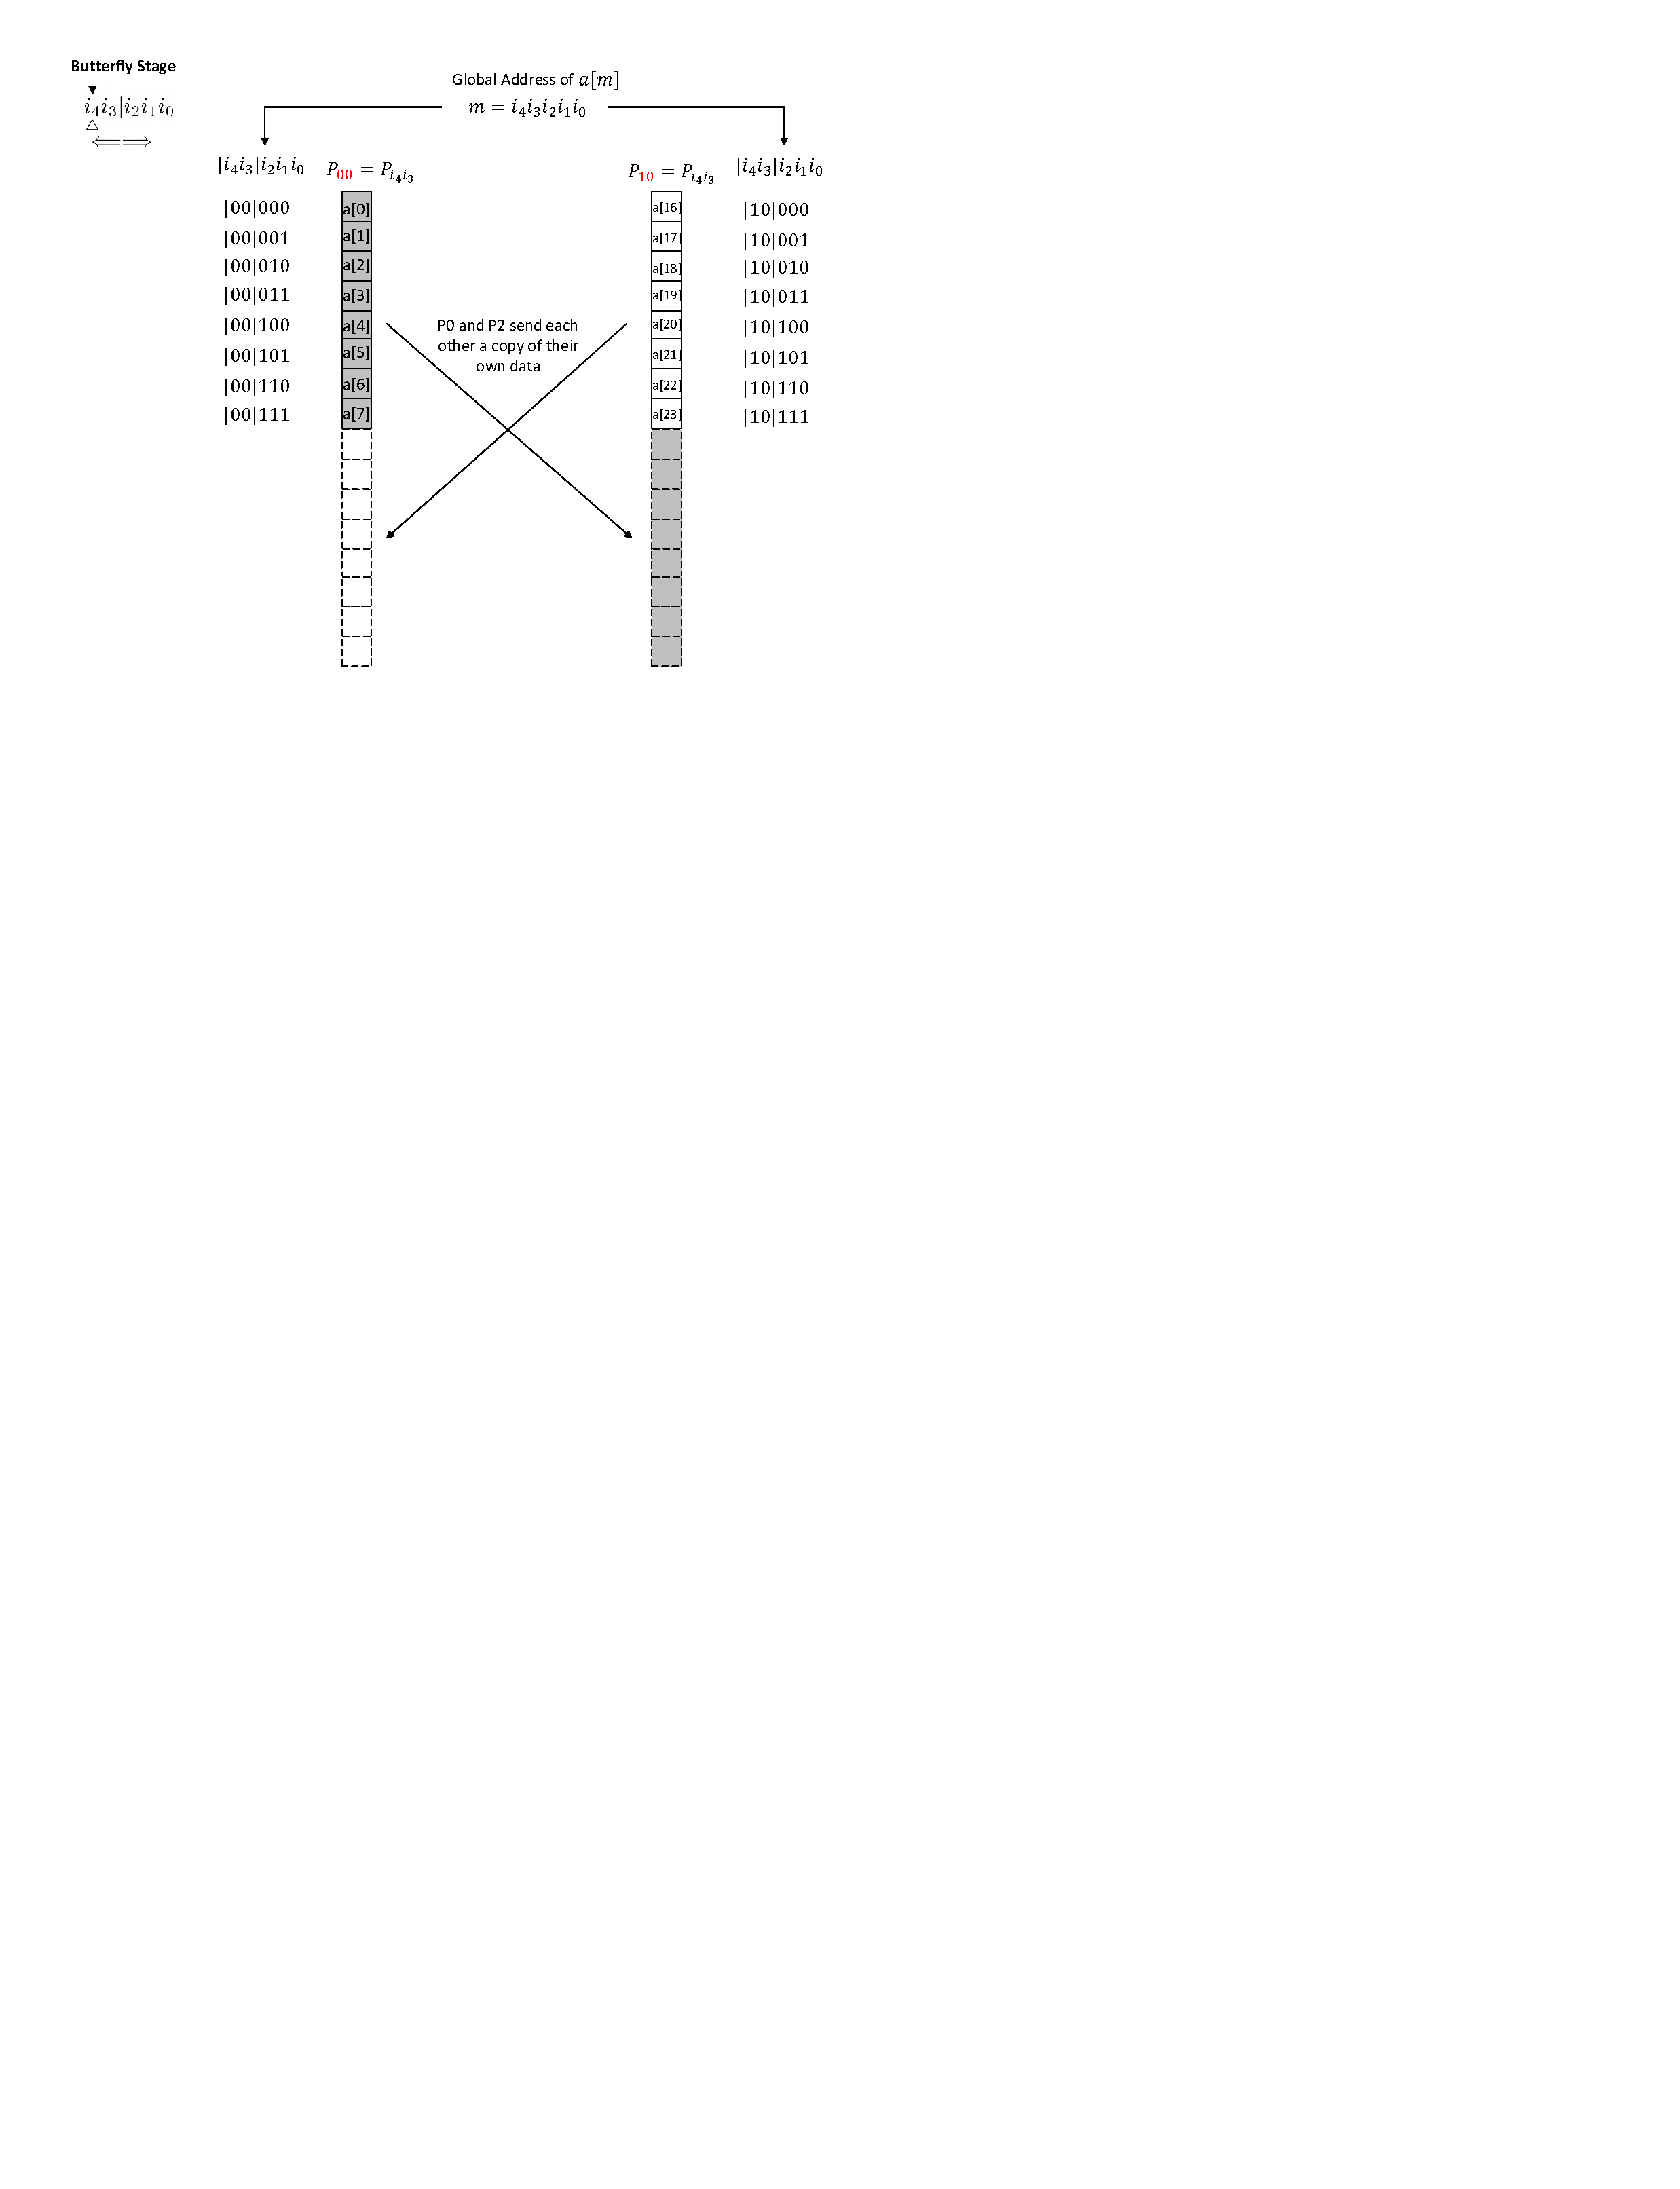
\includegraphics[width=\textwidth]{./fig/DataSwapWithoutPerm1.pdf}
\caption{In round-0, Data sent and received by processors $P_0$ and $P_2$}\label{fig:dataswap_without_perm1}
\end{subfigure}
\hspace{1em}
\begin{subfigure}[b]{.47\textwidth}\centering
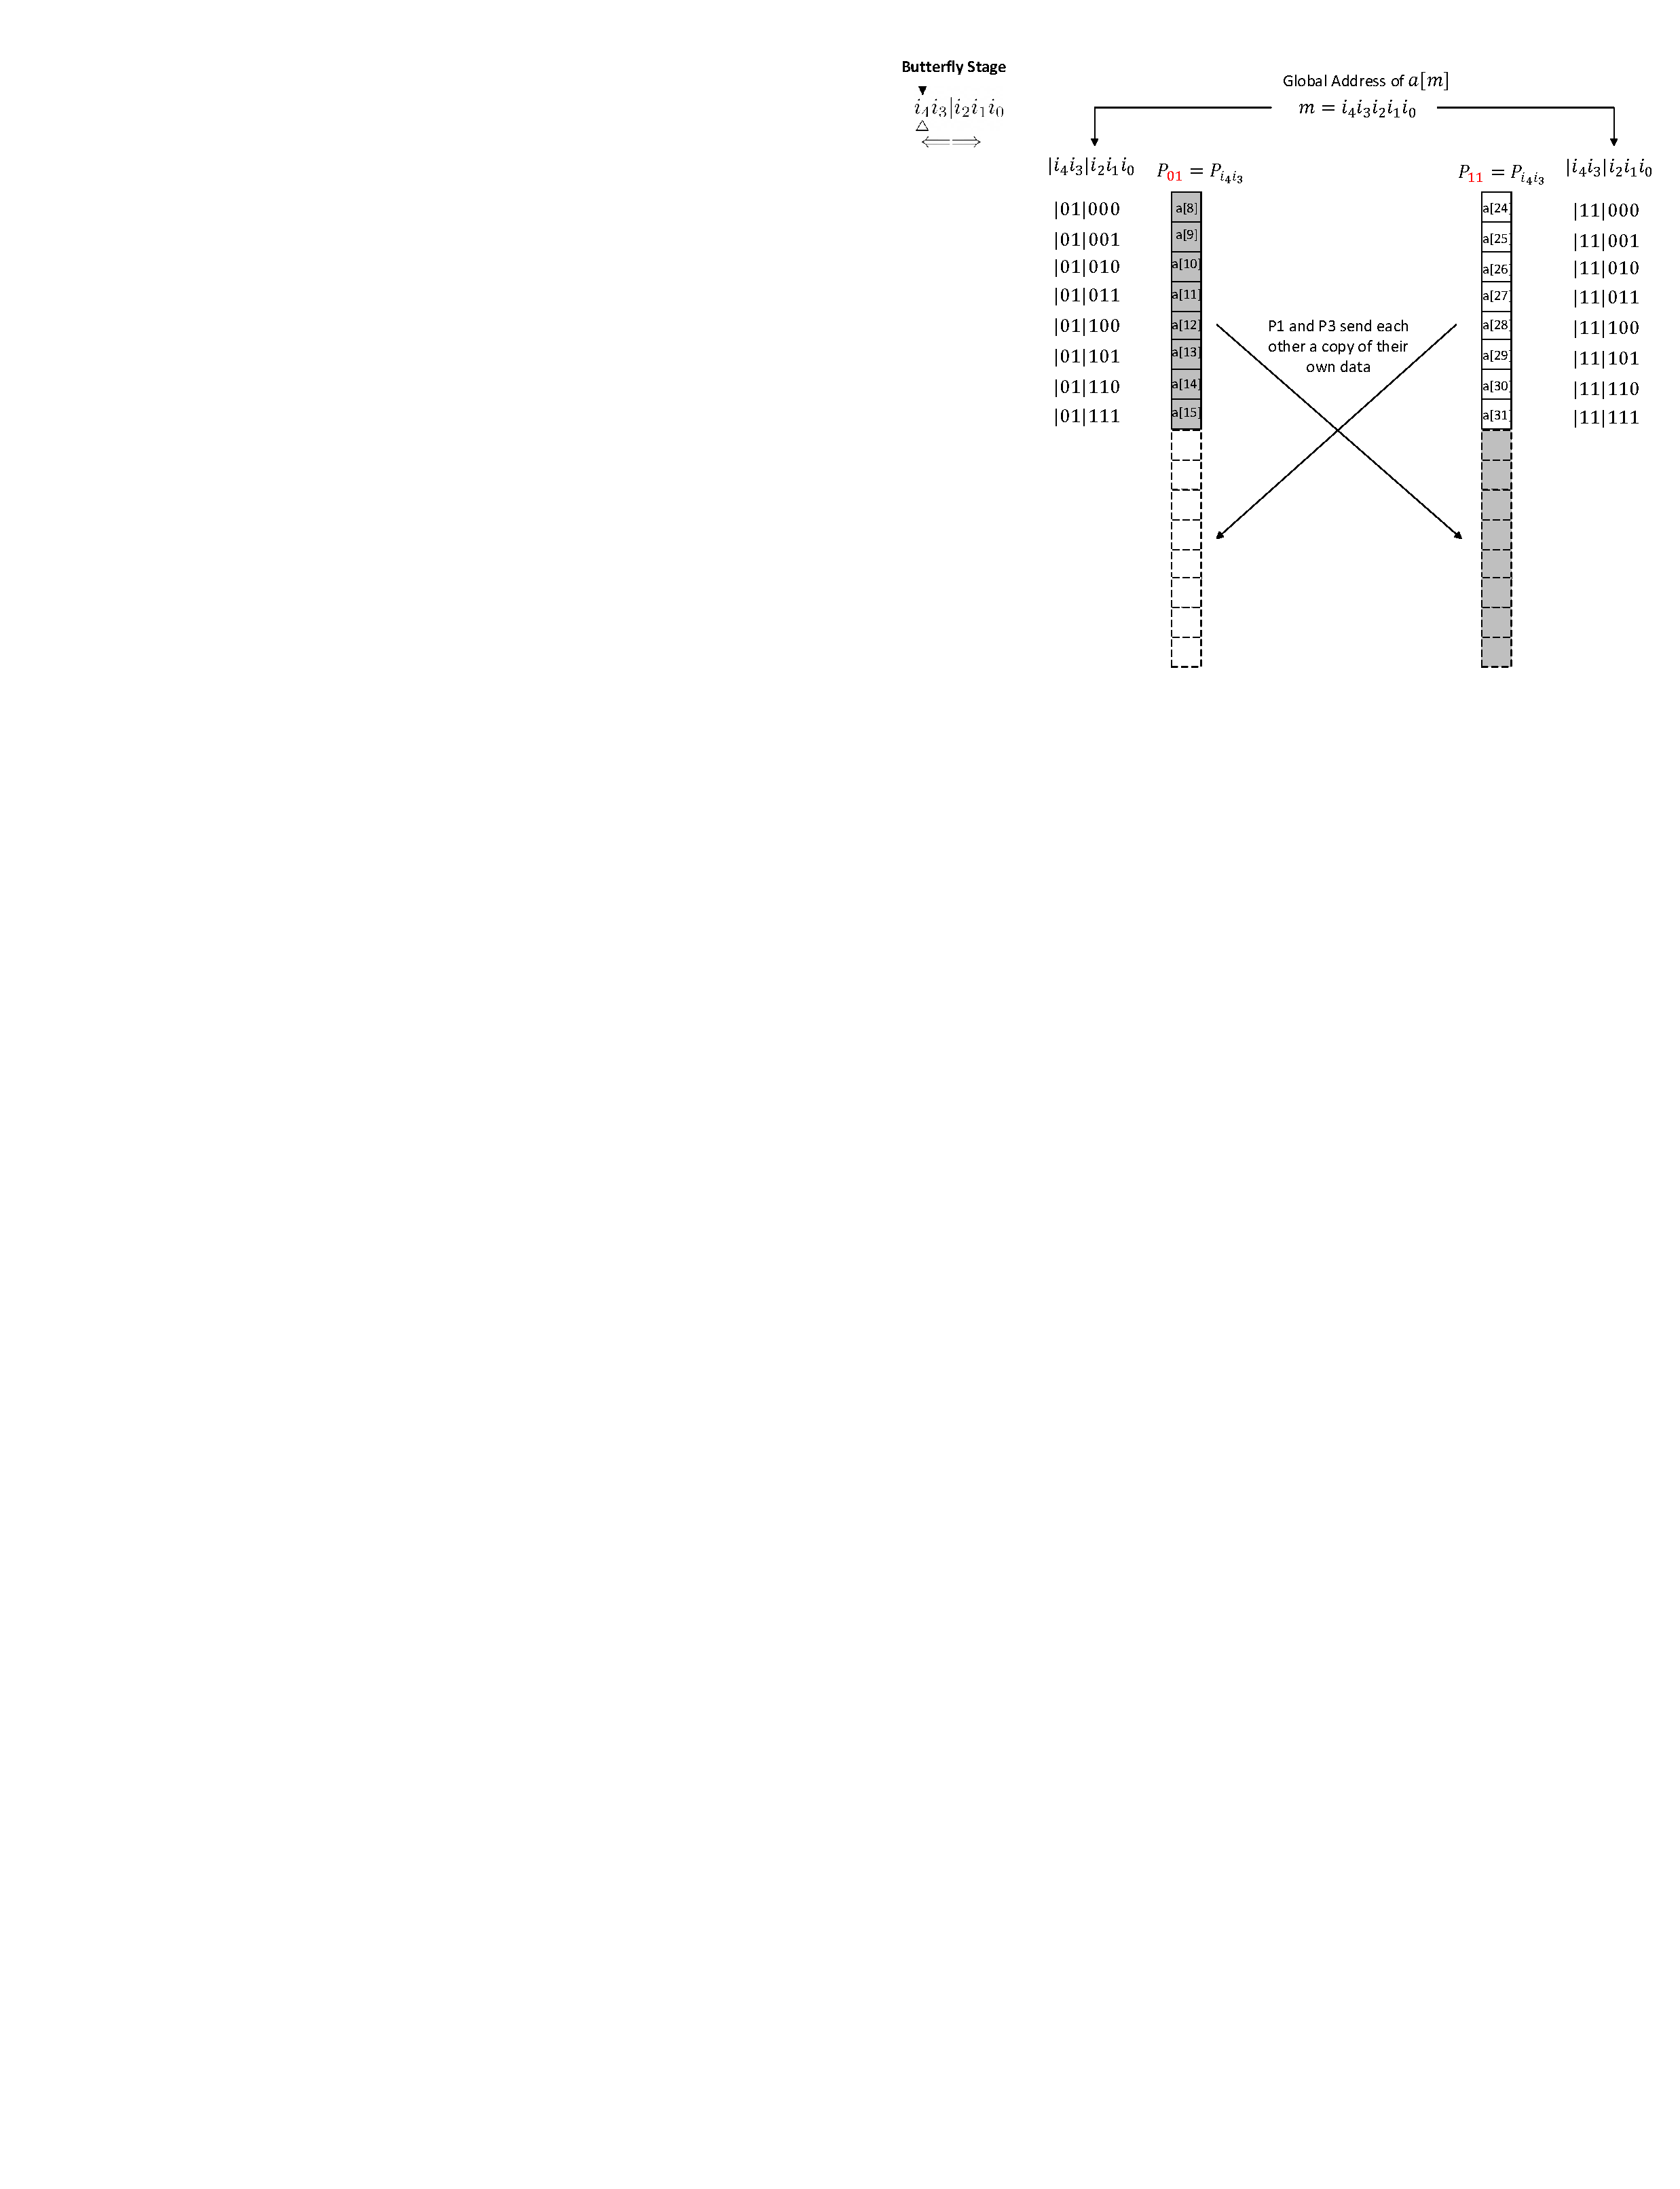
\includegraphics[width=\textwidth]{./fig/DataSwapWithoutPerm2.pdf}
\caption{In round-0, Data sent and received by processors $P_1$ and $P_3$}\label{fig:dataswap_without_perm2}
\end{subfigure}

\begin{subfigure}[b]{0.47\textwidth}
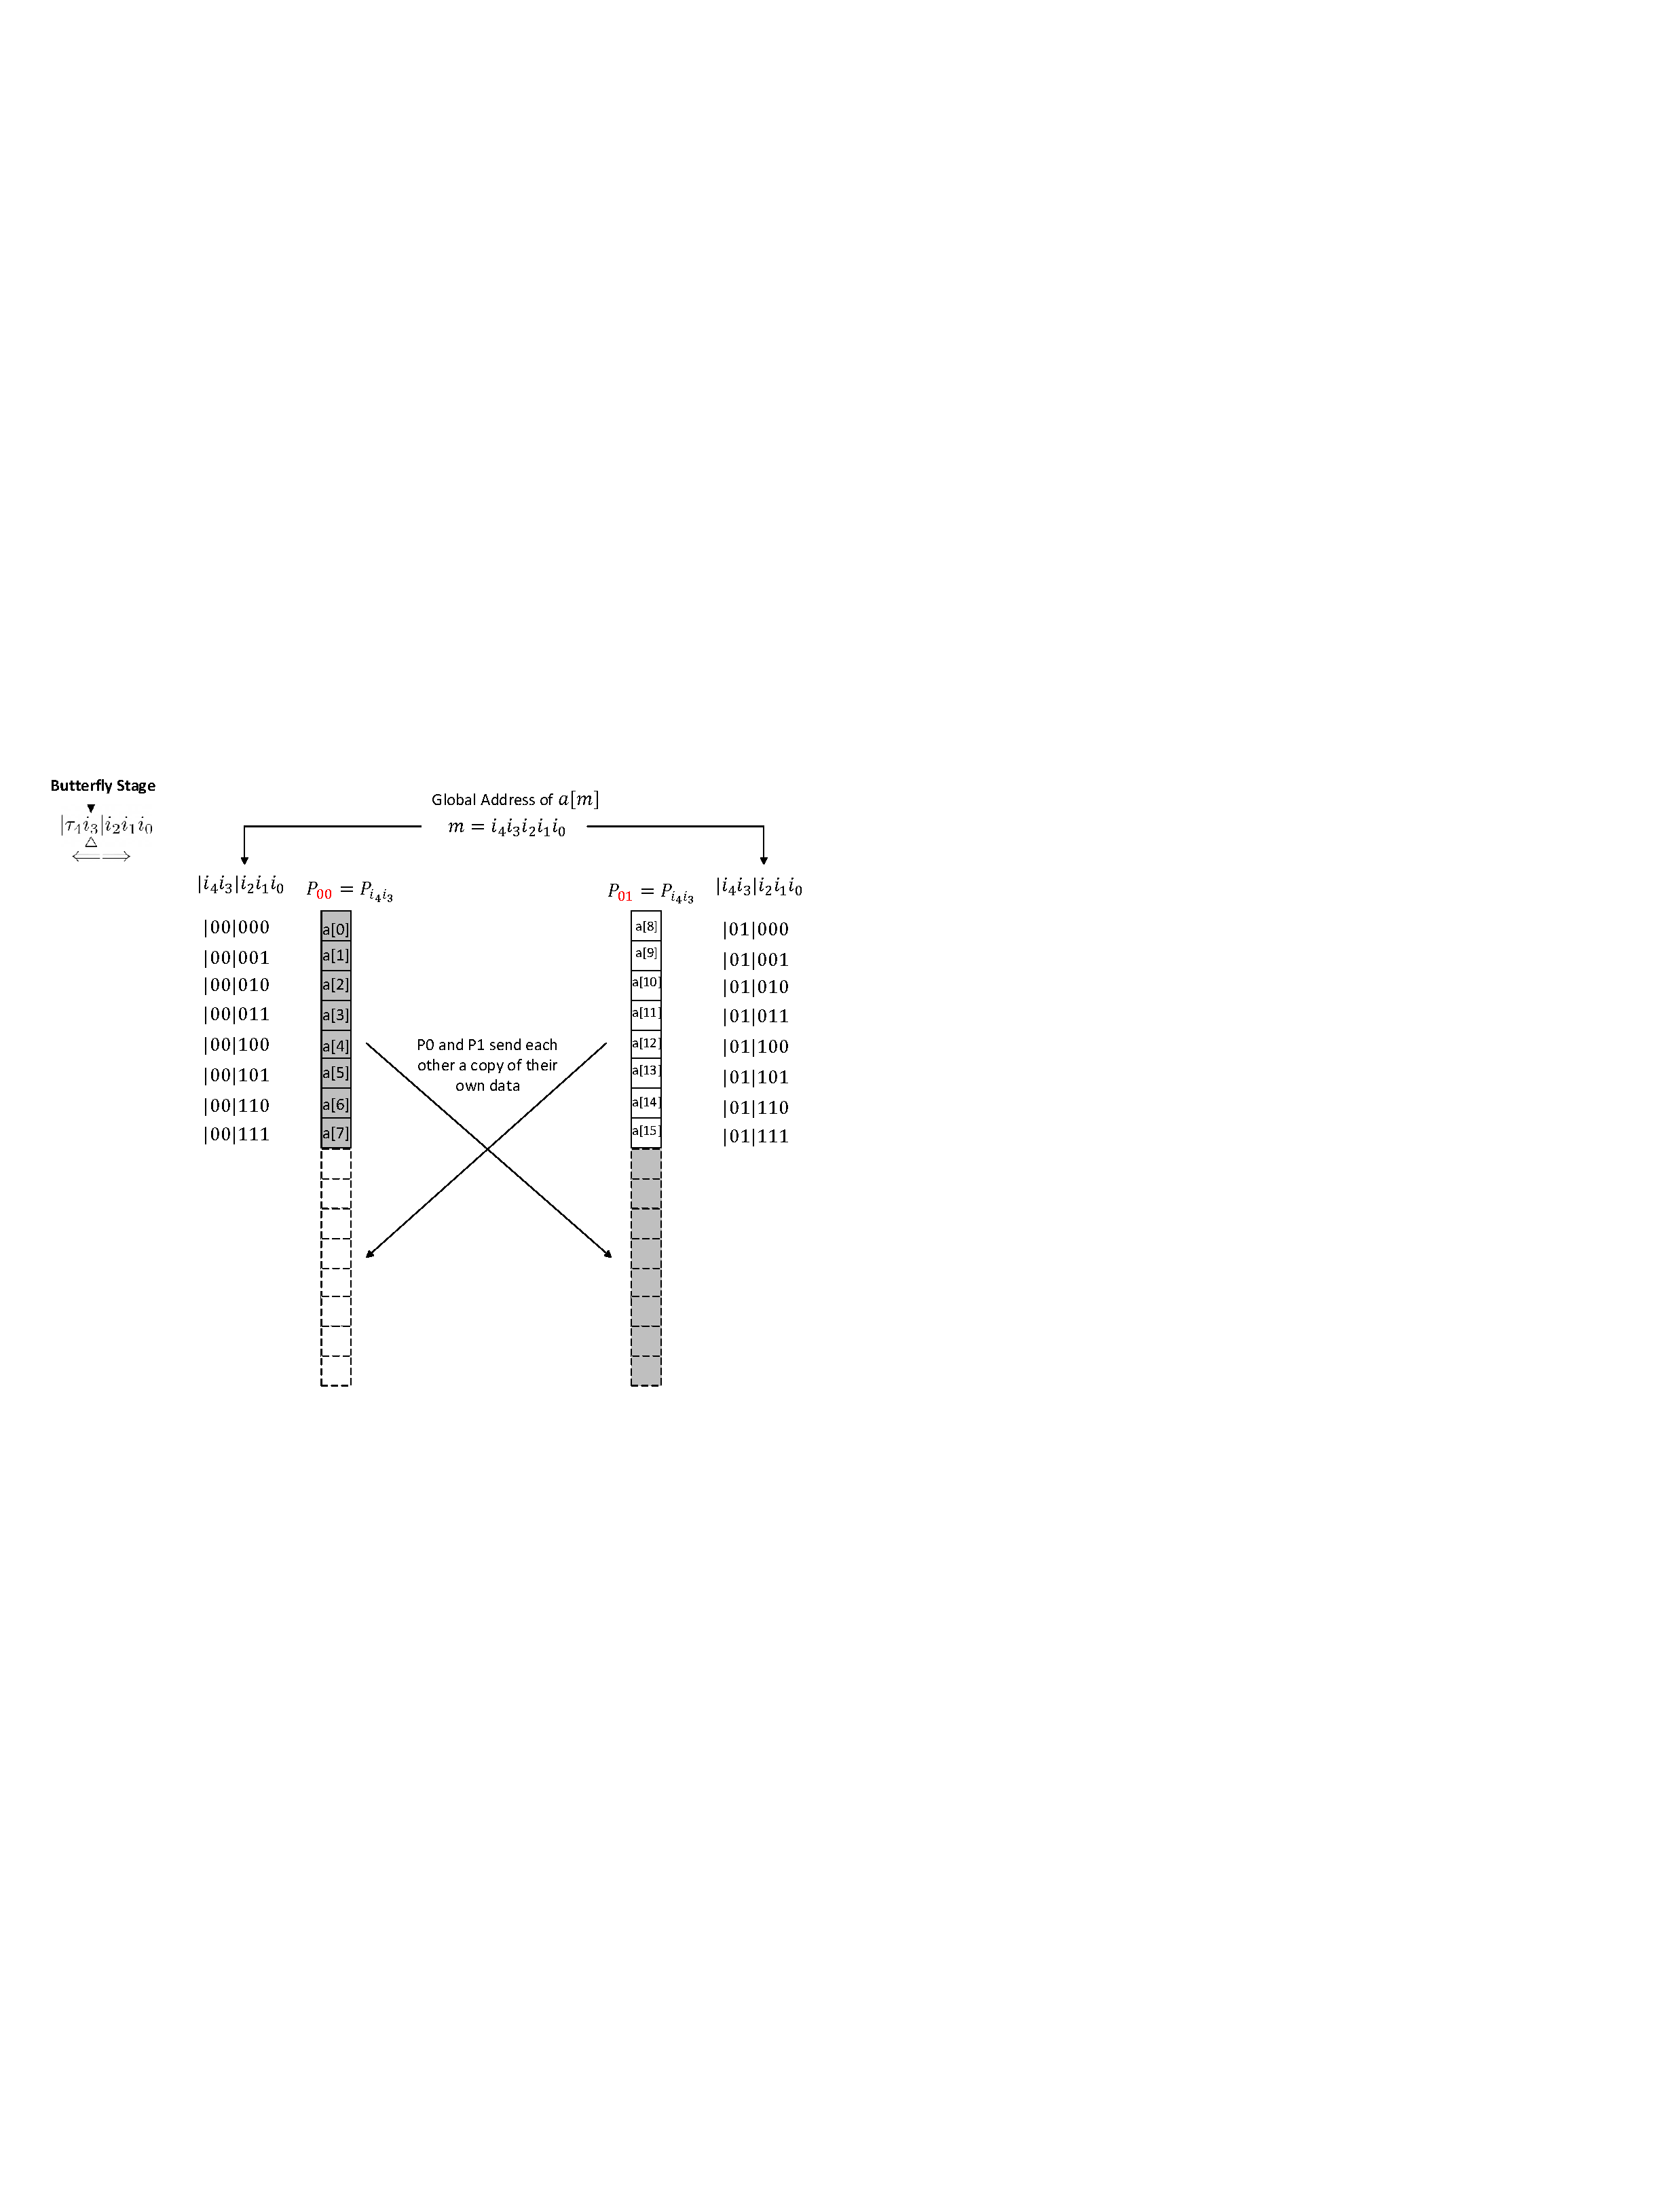
\includegraphics[width=\textwidth]{./fig/DataSwapWithoutPerm3.pdf}
\caption{In round-1, Data sent and received by processors $P_0$ and $P_1$}\label{fig:dataswap_without_perm3}
\end{subfigure}
\hspace{1em}
\begin{subfigure}[b]{.47\textwidth}\centering
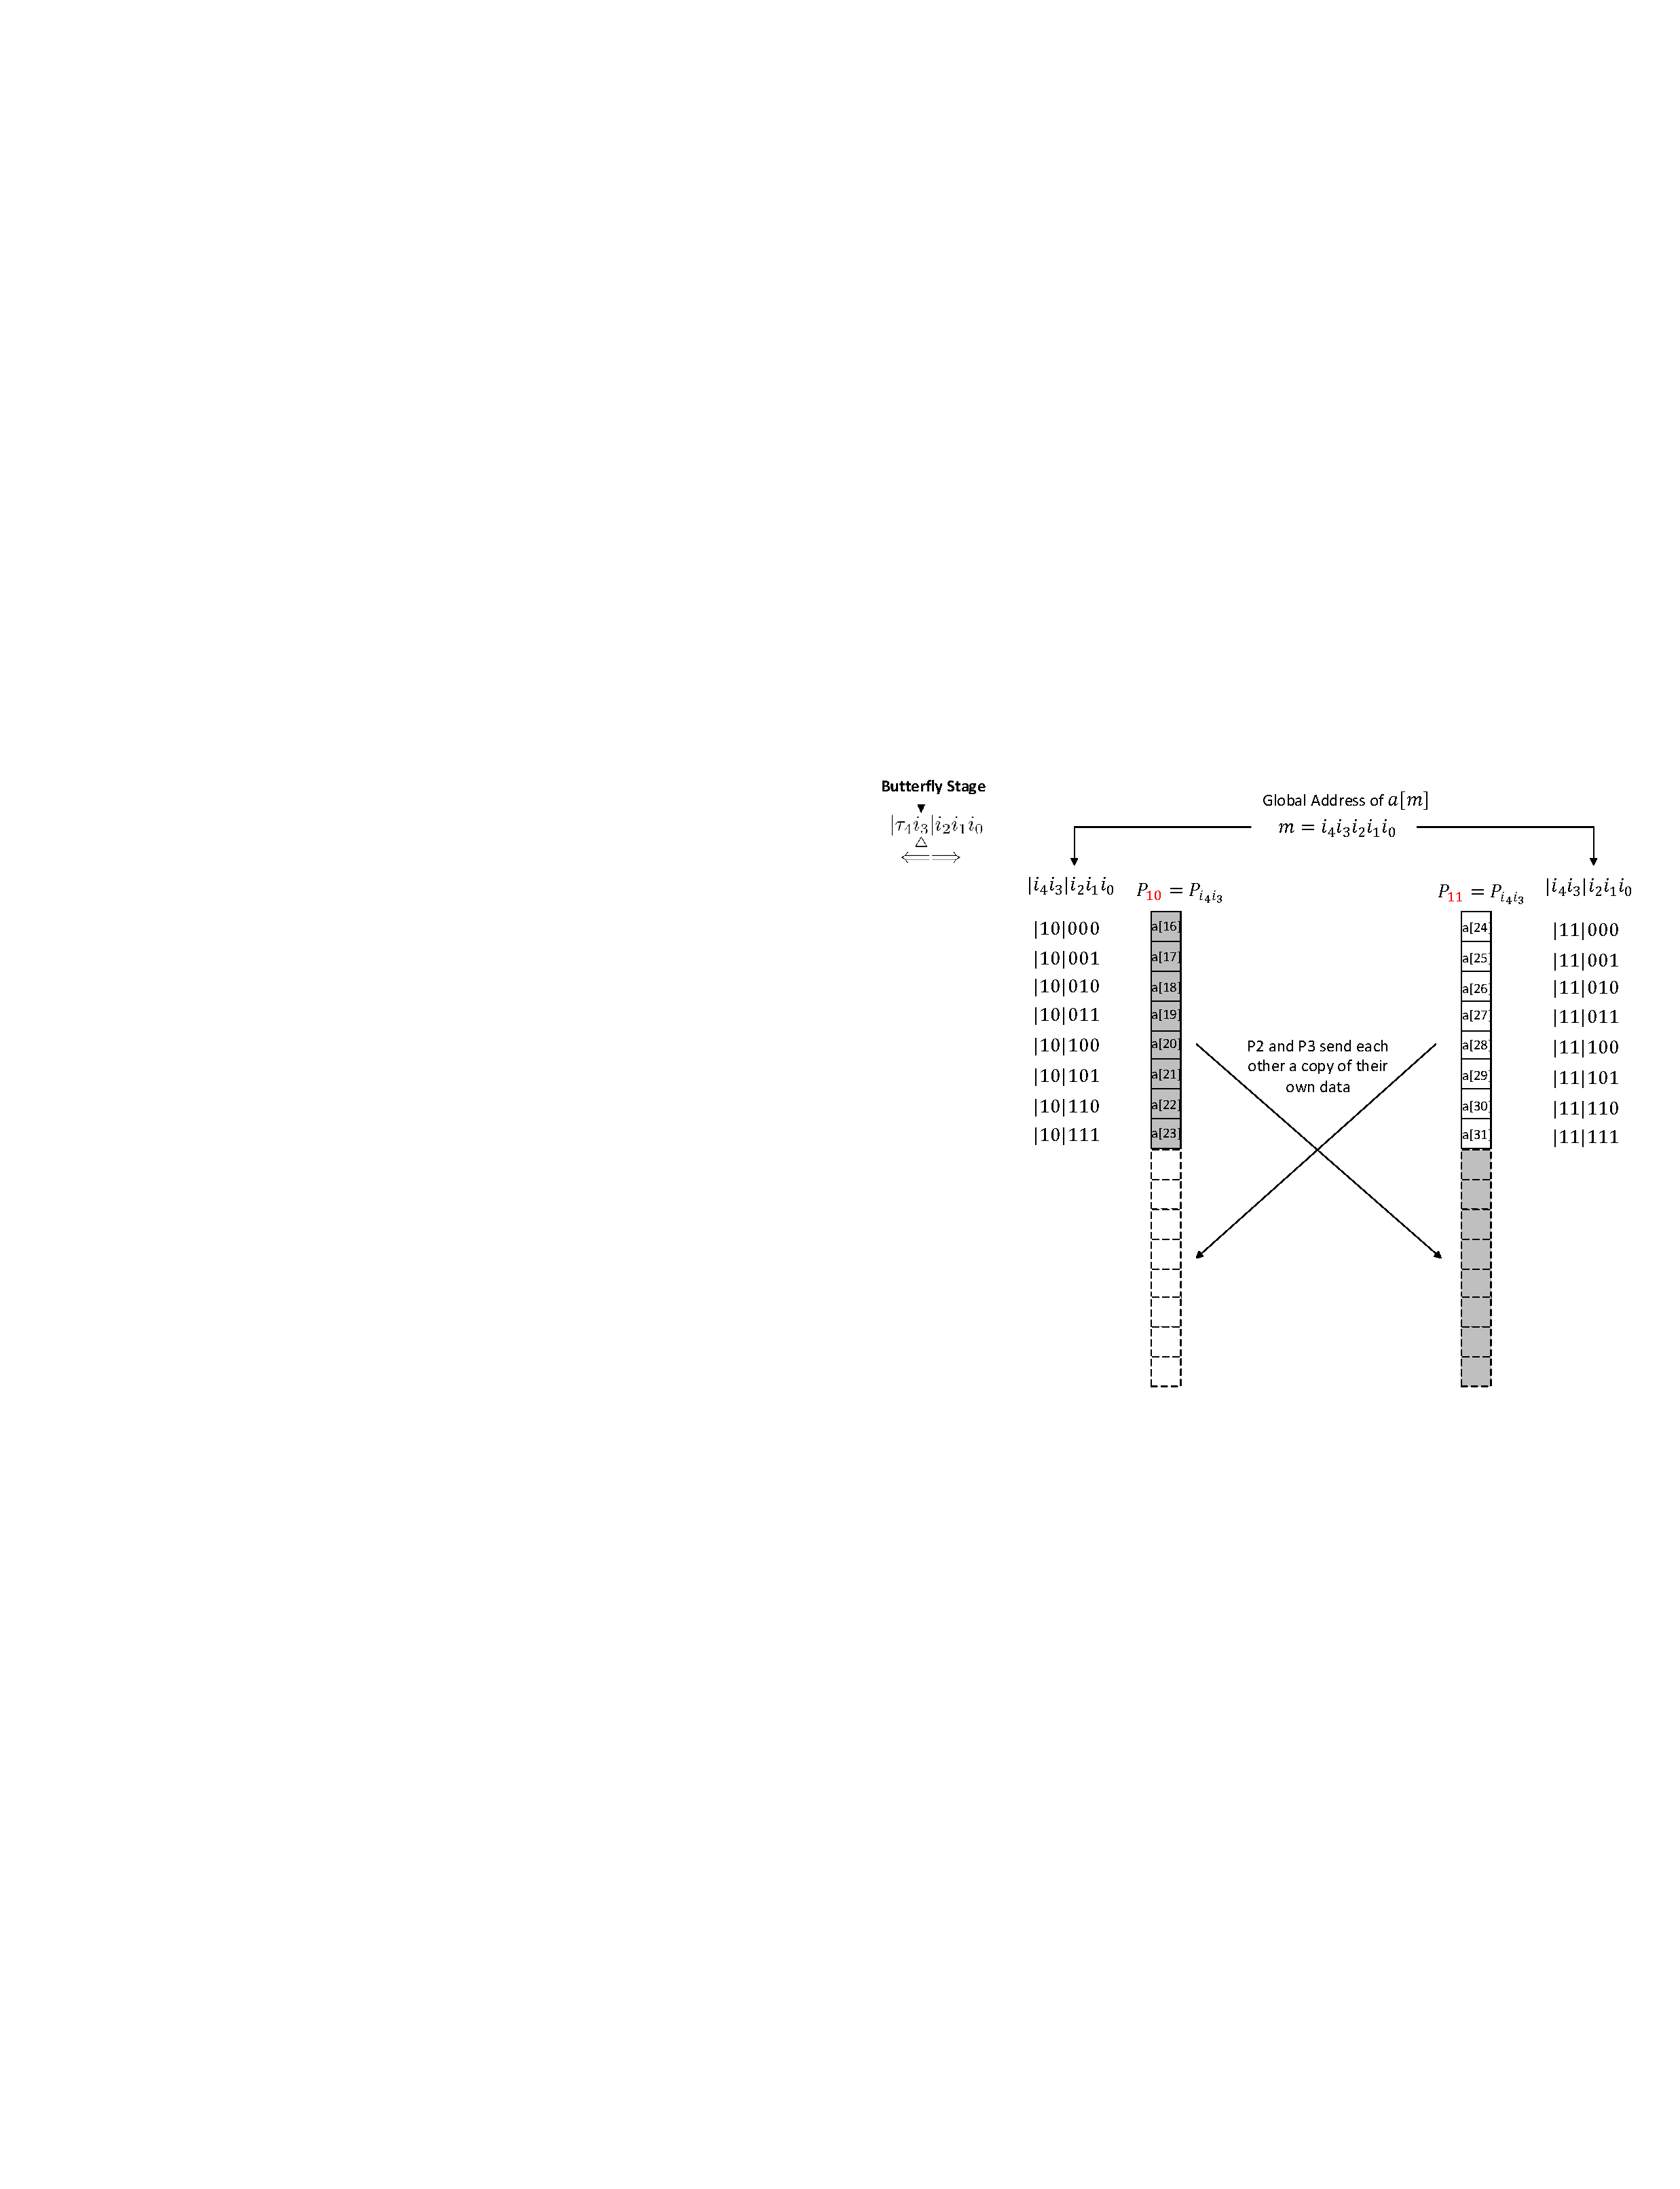
\includegraphics[width=\textwidth]{./fig/DataSwapWithoutPerm4.pdf}
\caption{In round-1, Data sent and received by processors $P_2$ and $P_3$}\label{fig:dataswap_without_perm4}
\end{subfigure}

\caption{An illustrative example for parallelizing in-place NTT($N=32,d=4$) without inter-processor permutations}\label{fig:dataswap_without_perm}
\end{figure*}

\textbf{Remarks} The parallel in-place NTT without inter-processor permutations approach employs \textit{data exchange between a pair of processors}. That is, one processor's initial complement of data may swap with that of another processor. With use of this type of data exchange, $N/d$ butterfly computations are performed in parallel at the cost of a number of $N/d$ data swaps per processor.  


\subsection{Second attempt: Parallel NTTs with Inter-processor permutations}
In this subsection, we discuss the class of parallel NTTs which employ inter-processor data permutations. Similar to the one presented in the previous subsection whih evenly distribute all butterfly computations among the processors, the new method also reduces the message length from $\frac{N}{d}$ elements to $\frac{1}{2}\frac{N}{d}$ in each of the $log_2d+1$ concurrent message exchanges.

\textbf{Modified shorthand notation} The new idea can be explained using a familiar example: suppose that $N=32$, and a consecutive data map denoted by $|i_4i_3|i_2i_1i_0$ is used to distribute data among
the four processors. A shorthand notation must reflect both the permutation and the computation accomplished in the parallel NTT approach. The modified notation extends the previous notation used for parallel NTT without permutations approach, and represent the first stage of butterfly computation as follows:

\begin{table}[h!]\begin{center}
\scalebox{0.8}{\begin{tabular}{c c}
\hline
$|i_4i_3|i_2i_1i_0$ & $|\underset{\triangle}{i_2}i_3|\underset{\triangle}{\overset{\blacktriangledown}{i_4}}i_1i_0$\\
Initial Map   &   $\longleftarrow\longrightarrow$\\
\hline
\end{tabular}}
\end{center}\end{table}

In the initial map (before performing the first stage butterfly computation), the input data are distributed as the element $a_{i_4i_3i_2i_1i_0}$ can be found in $A[i_2i_1i_0]$ in processor $P_{i_4i_3}$. For example, $a[19]=a_{19}$ is shown to be initially in $A[3]$ in $P_2$ in Fig.~\ref{fig:dataswap_with_perm1}, $a[14]=a_{14}$ is relocated to $A[2]$ in $P_3$ after the inter-processor permutation shown in Fig.~\ref{fig:dataswap_with_perm2}.


When bit $i_4$ in the PID and bit $i_2$ in the local $M$ switch their positions in the shorthand notation, the mapping is changed to $|i_2i_3|i_4i_1i_0$, which means that the data in
$a[i_4i_3i_2i_1i_0]$ can now be found in $A[i_4i_1i_0]$ in $P_{i_2i_3}$. For example, $a[19]=a_{19}$ is relocated to $A[7]$ in $P_0$ after the inter-processor permutation shown in Fig.~\ref{fig:dataswap_with_perm1}, $a[14]=a_{14}$ is relocated to $A[2]$ in $P_3$ after the inter-processor permutation shown in Fig.~\ref{fig:dataswap_with_perm2}.


To identify the one half of the data each processor must send out, the symbol $\triangle$ is used to label two different bits: the bit $\underset{\triangle}{i_k}$, which has just been permuted from PID
to Local $M$, and the bit $\underset{\triangle}{i_{\ell}}$, which has just been permuted from Local $M$ to the PID. In the example above, $\underset{\triangle}{i_4}$ and $\underset{\triangle}{i_2}$ have switched their respective positions in the PID and the Local $M$.

\begin{figure*}[!tb]
\centering
\begin{subfigure}[b]{.95\textwidth}
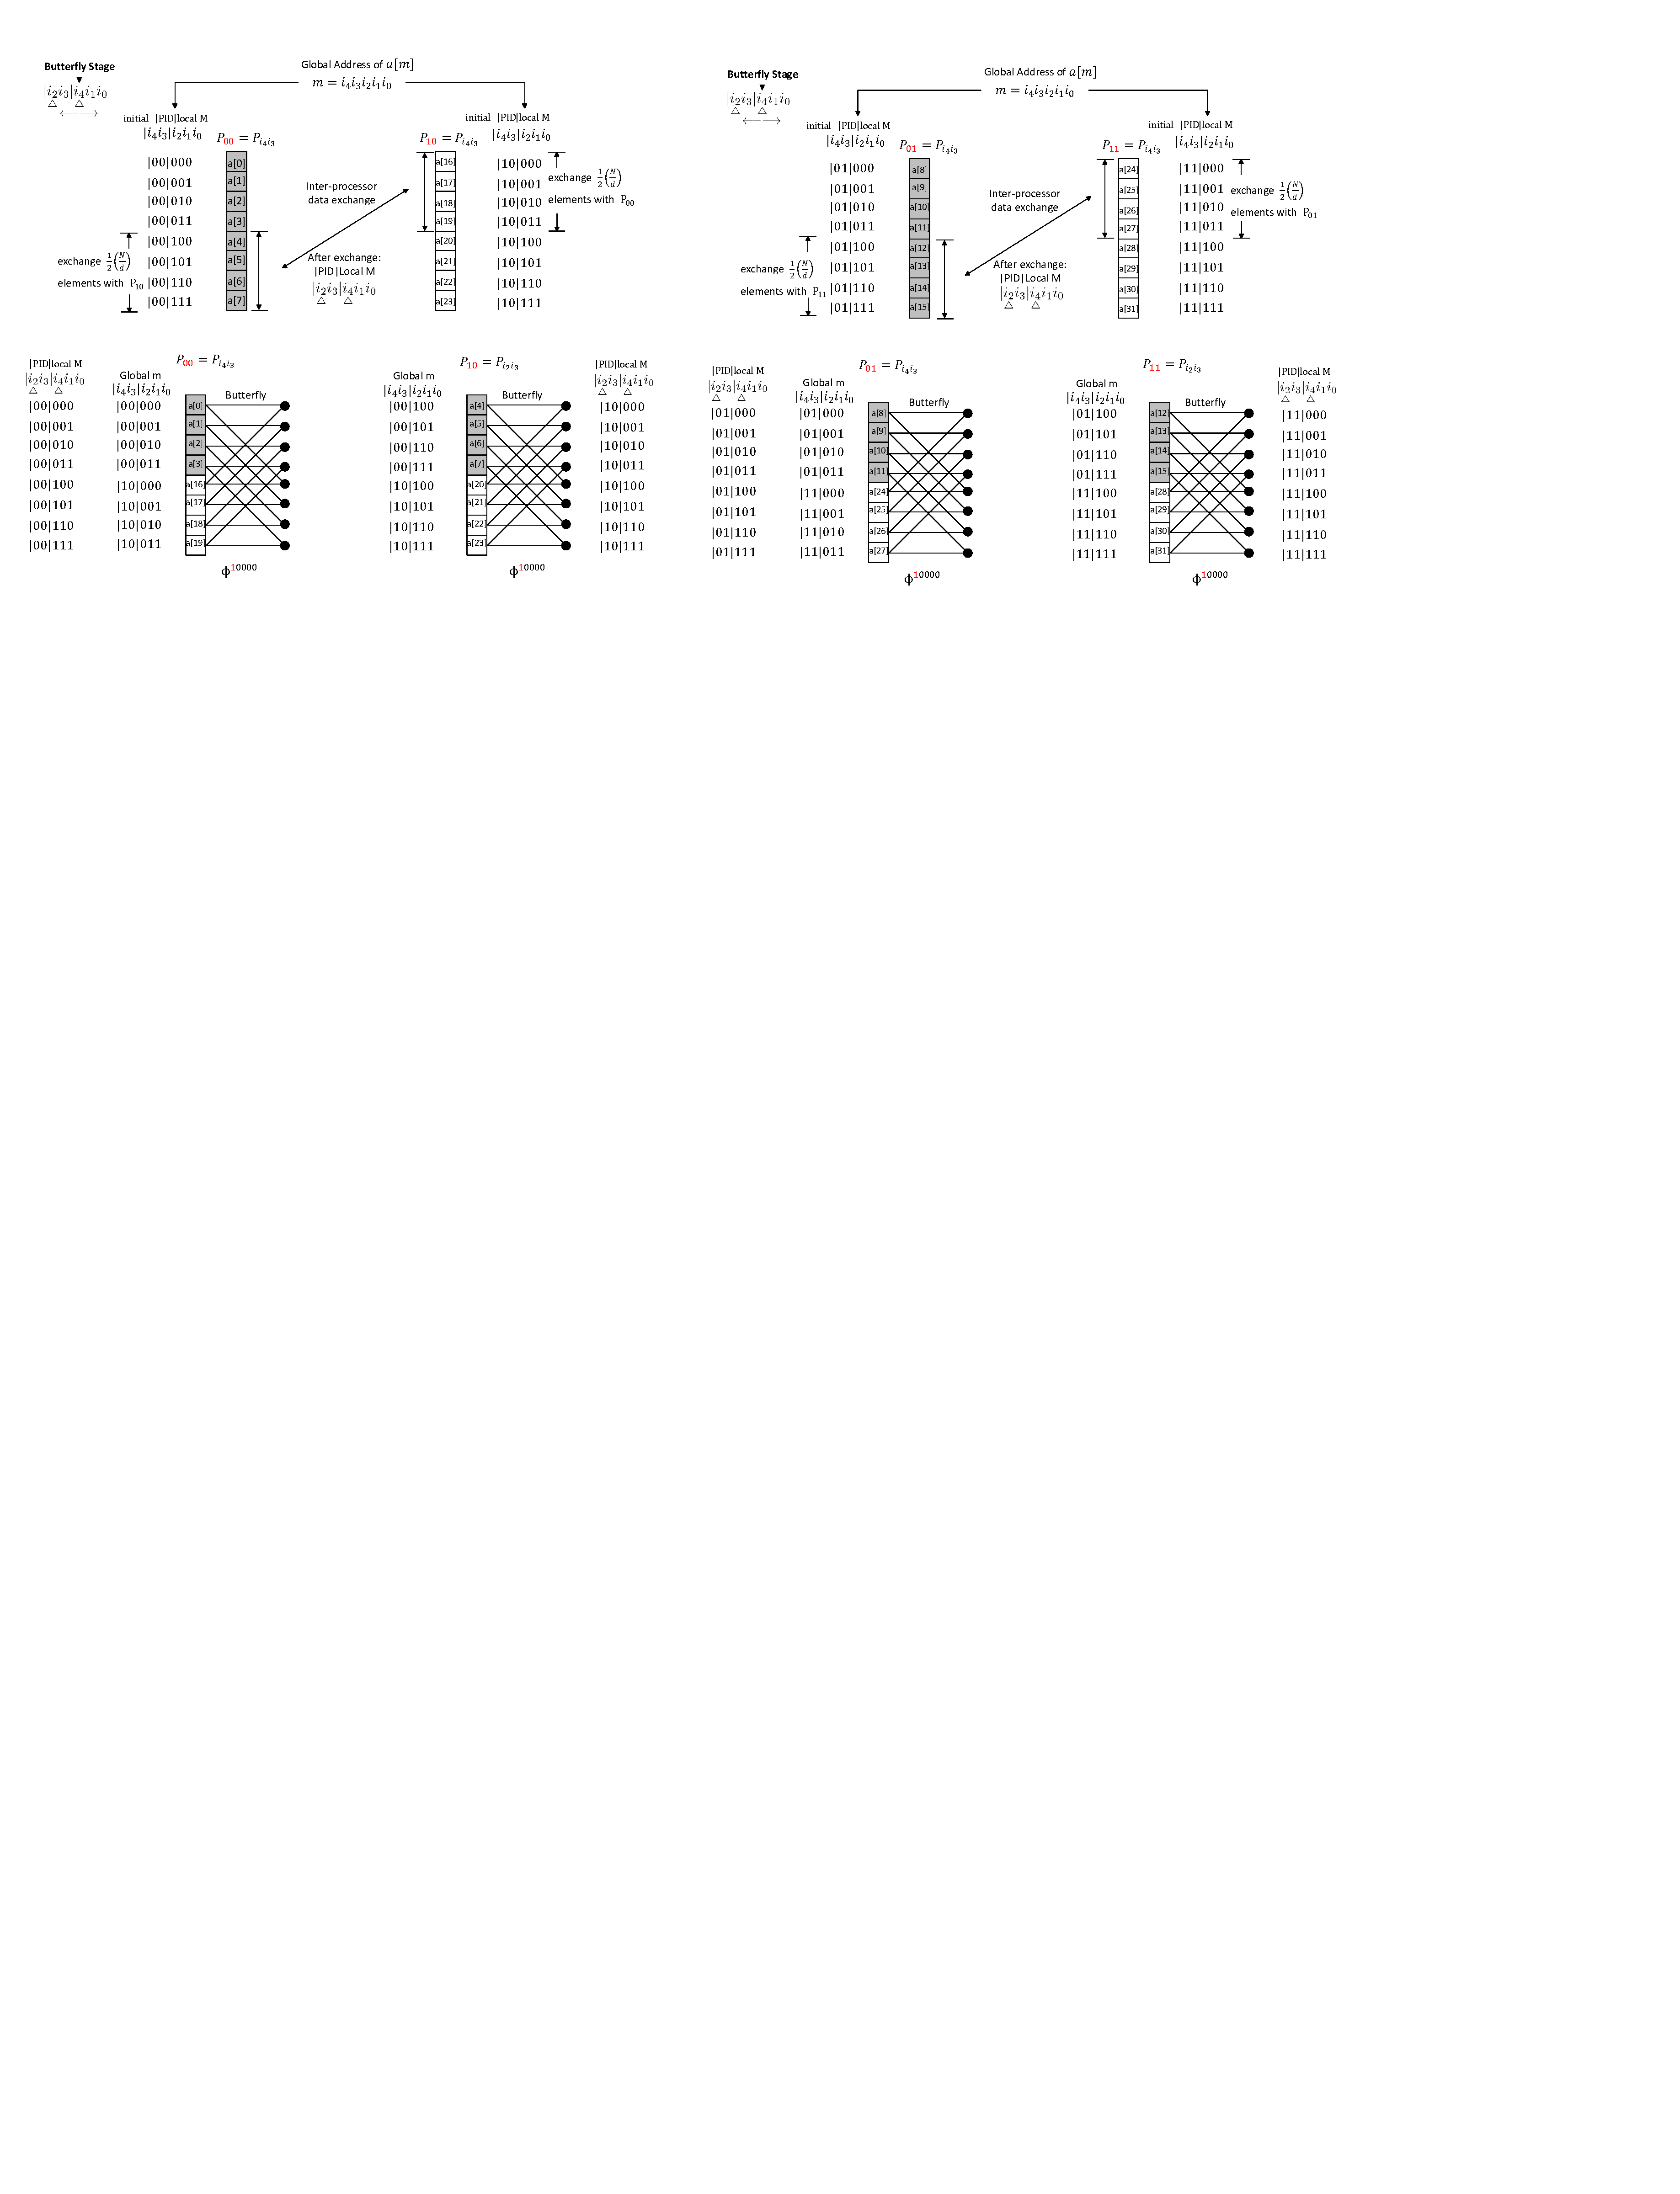
\includegraphics[width=\textwidth]{./fig/DataSwapWithPerm1.pdf}
\caption{In round-0, $DIT_{NR}$ butterfly computation with data migration between processors $P_0$ and $P_2$, and $P_1$ and $P_3$, respectively}\label{fig:dataswap_with_perm1}
\end{subfigure}
\hspace{1em}
\begin{subfigure}[b]{.95\textwidth}\centering
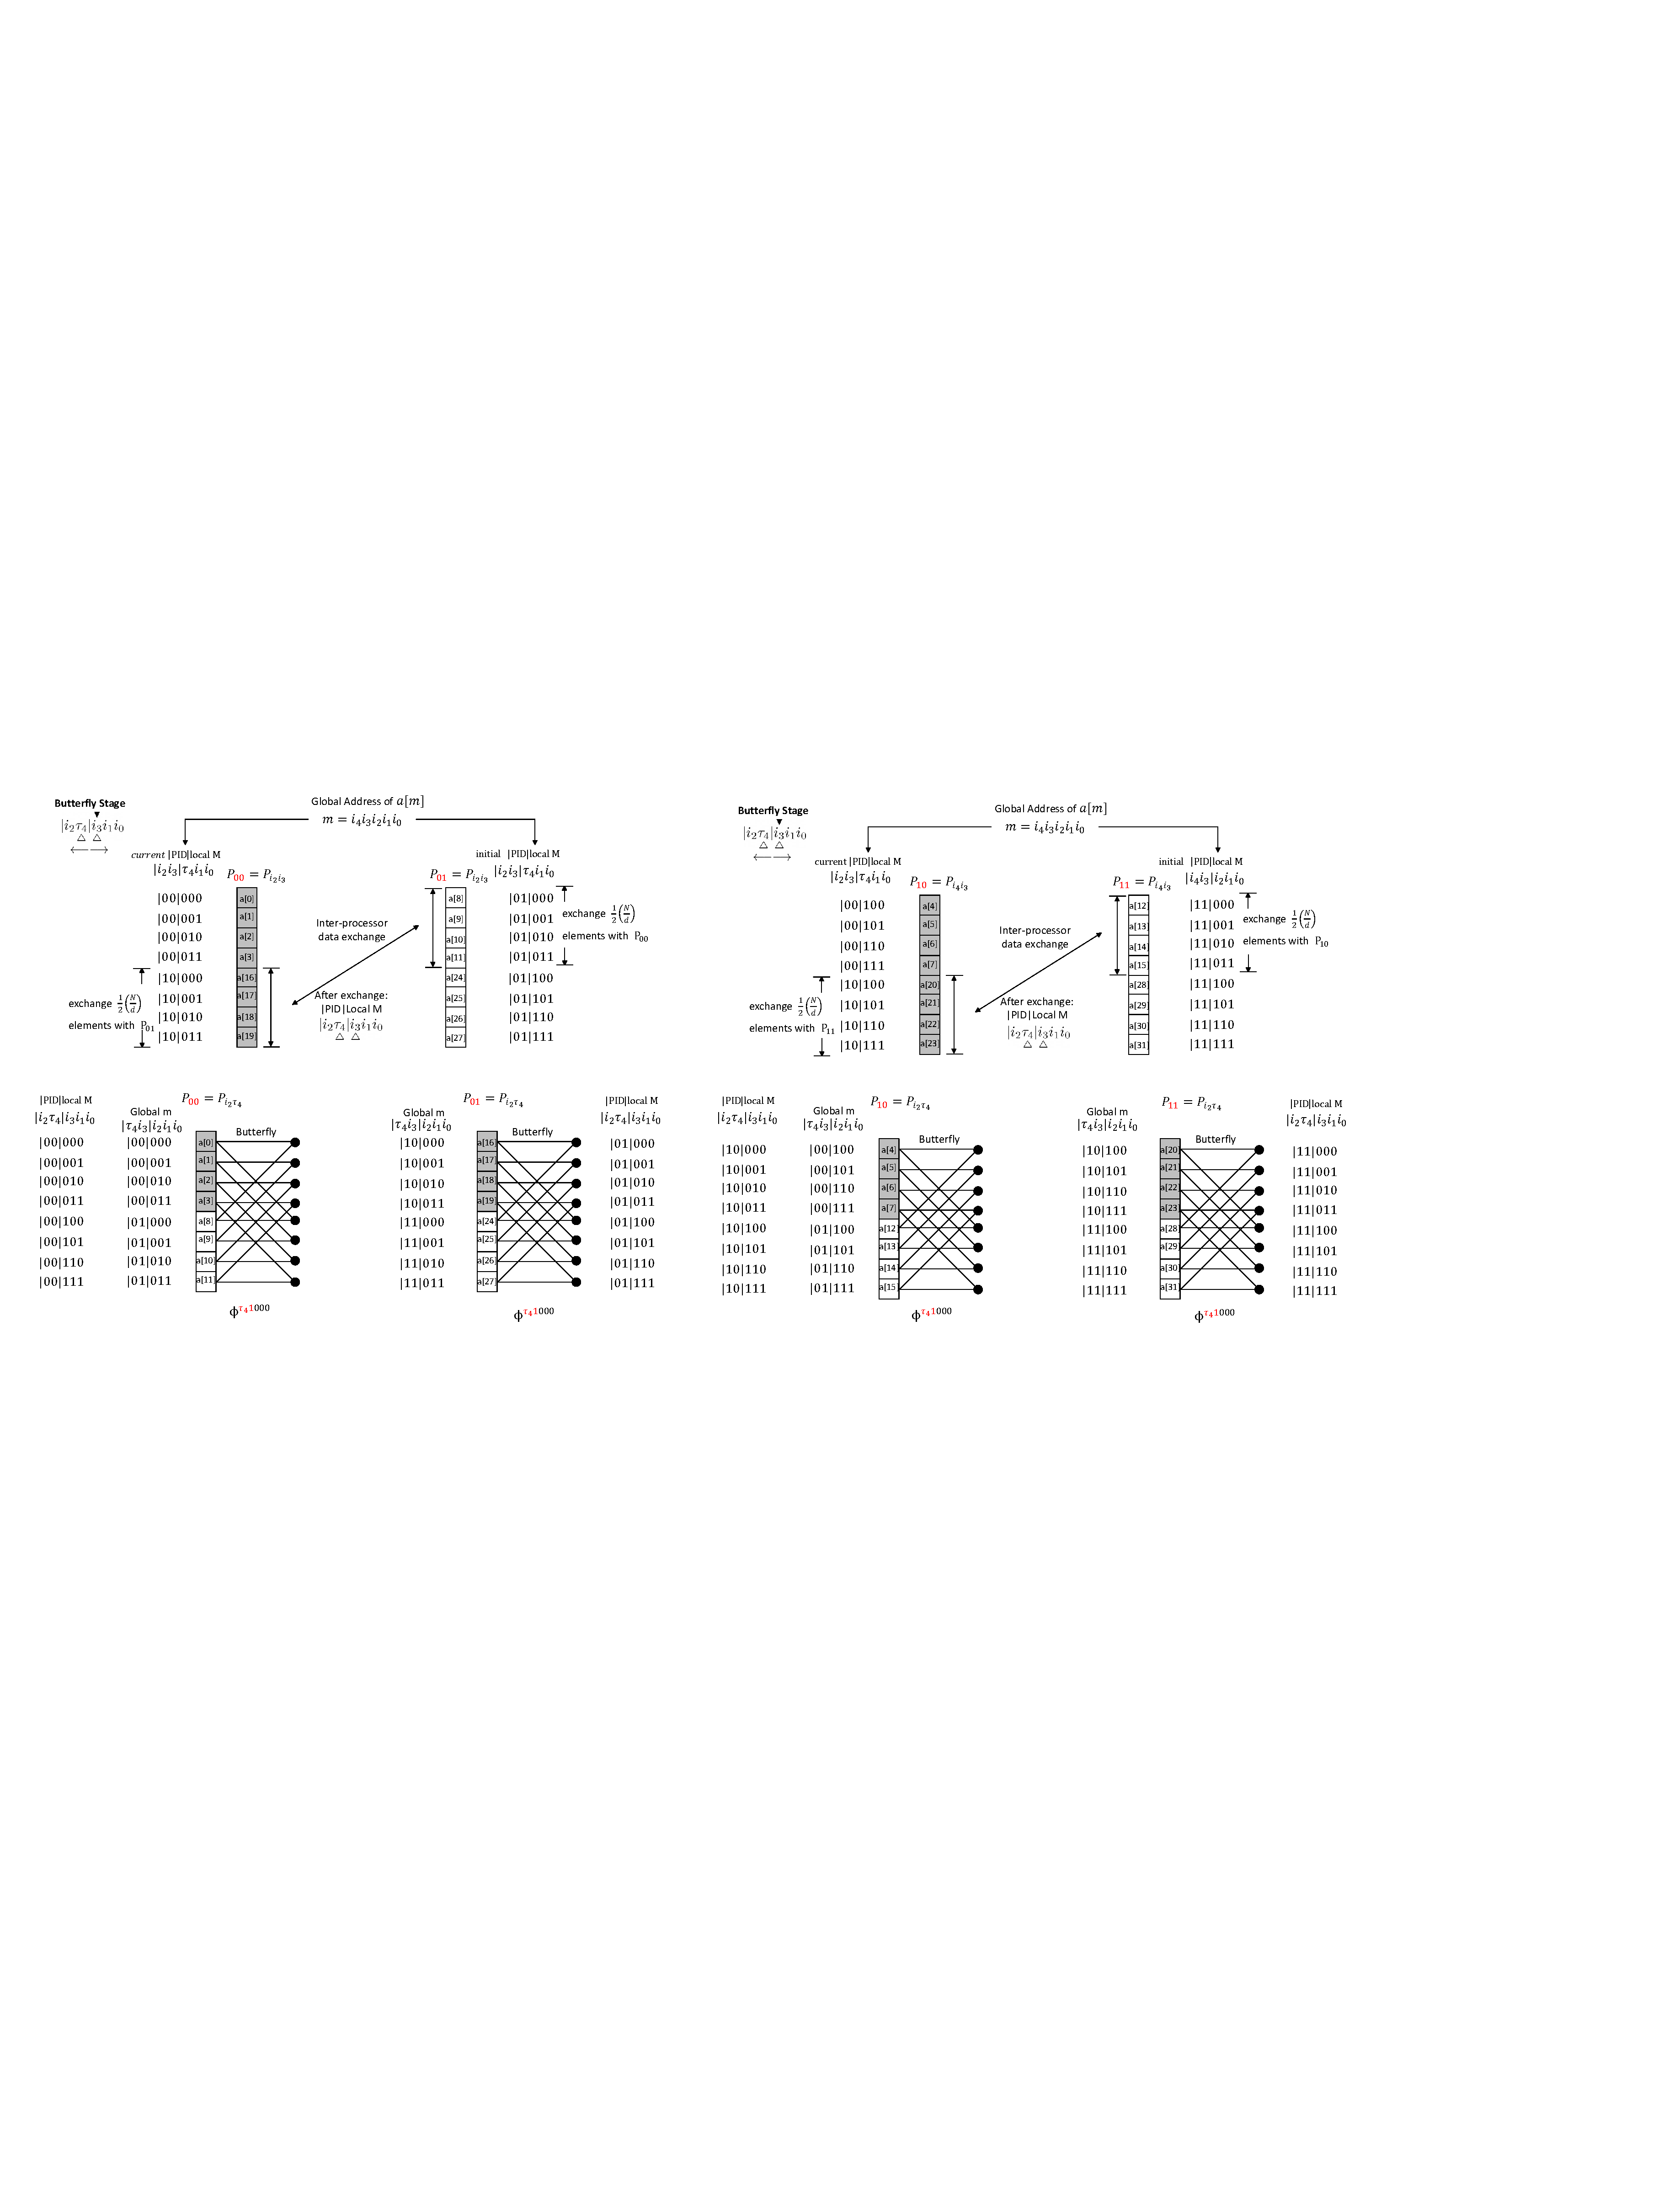
\includegraphics[width=\textwidth]{./fig/DataSwapWithPerm2.pdf}
\caption{In round-1, $DIT_{NR}$ butterfly computation with data migration between processors $P_0$ and $P_1$, and $P_2$ and $P_3$, respectively}\label{fig:dataswap_with_perm2}
\end{subfigure}
\hspace{1em}
\begin{subfigure}[b]{.95\textwidth}
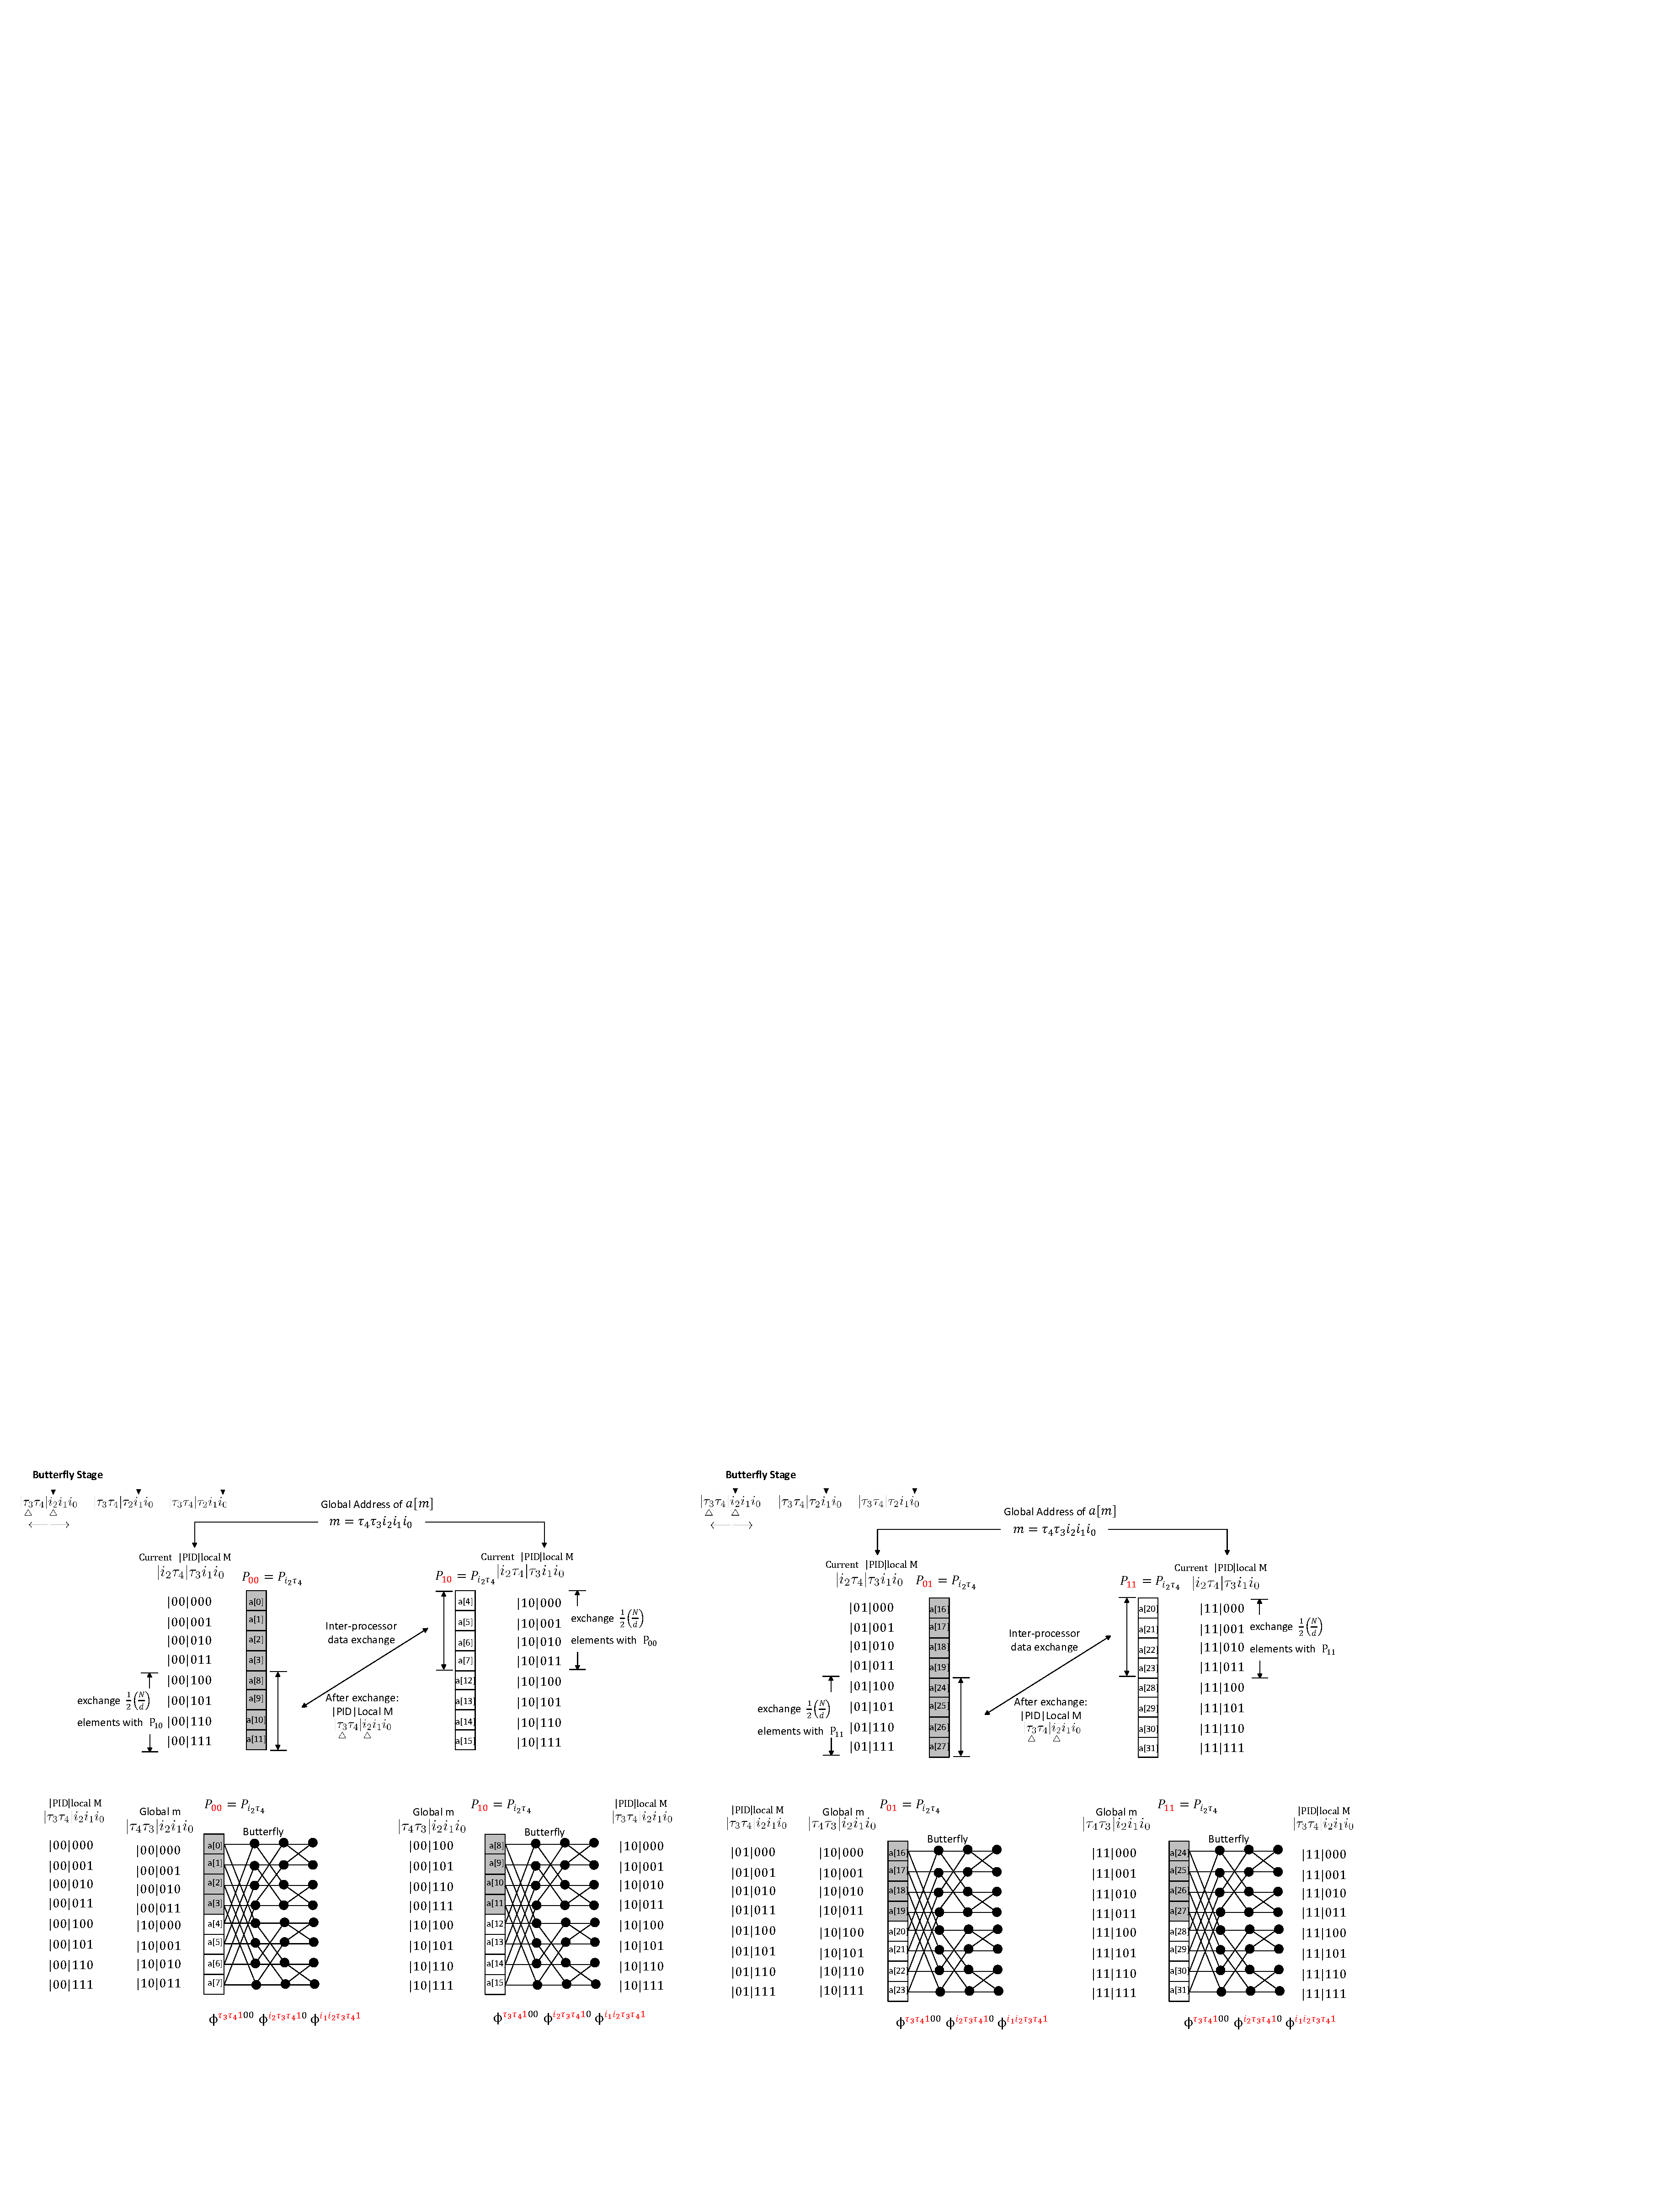
\includegraphics[width=\textwidth]{./fig/DataSwapWithPerm3.pdf}
\caption{In round-2/3/4, $DIT_{NR}$ butterfly computation with data migration between processors $P_0$ and $P_2$, and $P_1$ and $P_3$, respectively}\label{fig:dataswap_with_perm3}
\end{subfigure}
\caption{An illustrative example for parallelizing in-place NTT($N=32,d=4$) with inter-processor permutations}\label{fig:dataswap_with_perm}
\end{figure*}

Because $i_k$ was in PID before the switch, $i_k=1$ in one processor, and $i_k=0$ in the other processor. On the other hand, because $i_{\ell}$ was in Local $M$ before the switch, $i_{\ell}=0$ for half of the data, and $i_{\ell}=1$ for another half of the data. Consequently, the value of $i_k$, the PID bit, is equal to $i_{\ell}$, the local $M$ bit, for half of the data elements in each processor, and the notation which represents the switch of these two bits identifies both the PID of the other processor as well as the data to be sent out or received. To depict exactly what happens, the data exchange between two processors and the butterfly computation represented by $|\underset{\triangle}{i_2}i_3|\underset{\triangle}{\overset{\blacktriangledown}{i_4}}i_1i_0$ is shown in its entirety in Fig.~\ref{fig:dataswap_with_perm1} and \ref{fig:dataswap_with_perm2}.


\textbf{The complete algorithm} Using the shorthand notation we have developed, the complete parallel algorithm corresponding to $DIT_{NR}$ NTT is represented below for the $N=32$ example.
\begin{table}[h!]\begin{center}
\scalebox{0.8}{\begin{tabular}{c c c c c c}
\hline
$|i_4i_3|i_2i_1i_0$ & $|\underset{\triangle}{i_2}i_3|\overset{\blacktriangledown}{\underset{\triangle}{i_4}}i_1i_0$ & $|i_2\underset{\triangle}{\tau_4}|\overset{\blacktriangledown}{\underset{\triangle}{i_3}}i_1i_0$ & $|\underset{\triangle}{\tau_3}\tau_4|\overset{\blacktriangledown}{\underset{\triangle}{i_2}}i_1i_0$ & $|\tau_3\tau_4|\tau_2\overset{\blacktriangledown}{i_1}i_0$ & $|\tau_3\tau_4|\tau_2\tau_1\overset{\blacktriangledown}{i_0}$\\
Initial Map   &   $\longleftarrow\longrightarrow$ &  $\longleftarrow\longrightarrow$ &  $\longleftarrow\longrightarrow$\\
\hline
\end{tabular}}
\end{center}\end{table}

To provide complete information for this example, the second stage of butterfly computation with inter-processor permutation is depicted in Fig.~\ref{fig:dataswap_with_perm2}; the third stage of butterfly computations with inter-processor permutation, together with the remaining two stages of local butterfly computations, are depicted in Fig.~\ref{fig:dataswap_with_perm3}.

To determine the data mapping for the output elements, observe the following.
\begin{itemize}
    \item The \textit{in-place} butterfly computation in the $DIT_{NR}$ algorithm ensures $a[i_4i_3i_2i_1i_0]=a_{i_4i_3i_2i_1i_0}^{(5)}=a_{i_0i_1i_2i_3i_4}$
    \item The final mapping $|\tau_3\tau_4|\tau_2\tau_1\tau_0$ indicates that the final content in $a[i_4i_3i_2i_1i_0]$ is now located in $a[i_2i_1i_0]$ in processor $P_{i_3i_4}$ (rather than the initially assigned processor $P_{i_4i_3}$)
\end{itemize}

Accordingly, the output data element $A_{i_0i_1i_2i_3i_4}$, which overwrites the data in $a[i_4i_3i_2i_1i_0]$, is finally contained in $A[i_2i_1i_0]$ in $P_{i_3i_4}$.


\begin{algorithm}[!tbh]
 \DontPrintSemicolon % Some LaTeX compilers require you to use \dontprintsemicolon instead
 \KwIn{a polynomial ring $R_q$, and NTT points $N$, input $\vec{a} = (a[0],\cdots, a[N-1])$}
 \KwOut{$NTT(\vec{a}))=\vec{A}=(A[0],\cdots,A[N-1])$}
    Initialize the hypercube connections between $d$ processors as described in Alg.~\ref{alg:descript_hypercube}\;
    Initialize the merged twiddle factor look-up table $\{w_i\}$ as described in Alg.~\ref{alg:descript_twiddlefactor}\;
    Initialize the data $a[i_{log_2N-log_2d-1}\cdots i_1i_0]$ in $P_{i_{log_2N-1}\cdots i_{log_2N-log_2d}}$ with $a[i_{log_2N-1}\cdots i_1i_0]$ for all $i_{log_2N-1},\cdots,i_0$\;
    \For{$j\leftarrow 0$ \KwTo $log_2d$}{ 
        exchange the first half of data in  $P_{i_{log_2N-1}\cdots i_{log_2N-1-j}\cdots i_{log_2N-log_2d}}$ w.r.t. $i_{log_2N-1-j}=0$ with the second half of data in  $P_{i_{log_2N-1}\cdots i_{log_2N-1-j}\cdots i_{log_2N-log_2d}}$ w.r.t. $i_{log_2N-1-j}=1$\;

        perform within each processor $P_{i_{log_2N-1}\cdots i_{log_2N-1-j}\cdots i_{log_2N-log_2d}}$ the $\frac{N}{2d}$ butterfly computations (round-$j$ butterfly)\;
    }
    \For{$j\leftarrow log_2d+1$ \KwTo $log_2N-1$}{ 
        perform within each processor $P_{i_{log_2N-1}\cdots i_{log_2N-1-j}\cdots i_{log_2N-log_2d}}$ the $\frac{N}{2d}$ butterfly computations (round-$j$ butterfly)\;
    }
    \Return {the data in all $d$ processors as $\vec{A}$\;}
 \caption{Parallel Hypercube NTT}\label{alg:descript_hypercube_ntt}
\end{algorithm}

\textbf{Twiddle Factor LUT Distribution} Let us disscuss in details on the distribution of the twiddle factor LUT within each butterfly processor here. In the first $log_d+1$ rounds of butterfly computations, memory swapping occurs and each butterfly processor utilizes only $1$ twiddle factor; in the next $logN-logd-1$ rounds, no memory swapping occurs and the number of twiddle factors utilized in eah butterfly processor increases exponentially (starting with $2$). Therefore, the total number of twiddle factors (the depth of twiddle factor LUT) in each processor is:
\[
    \sum_{i=1}^{logd+1}1 + \sum_{i=1}^{logN-logd-1}2^i=\frac{N}{d}+logd-1
\]

\subsection{Butterfly Processor}\label{sec:butterfly processor}
\begin{figure*}[!tb]
\centering
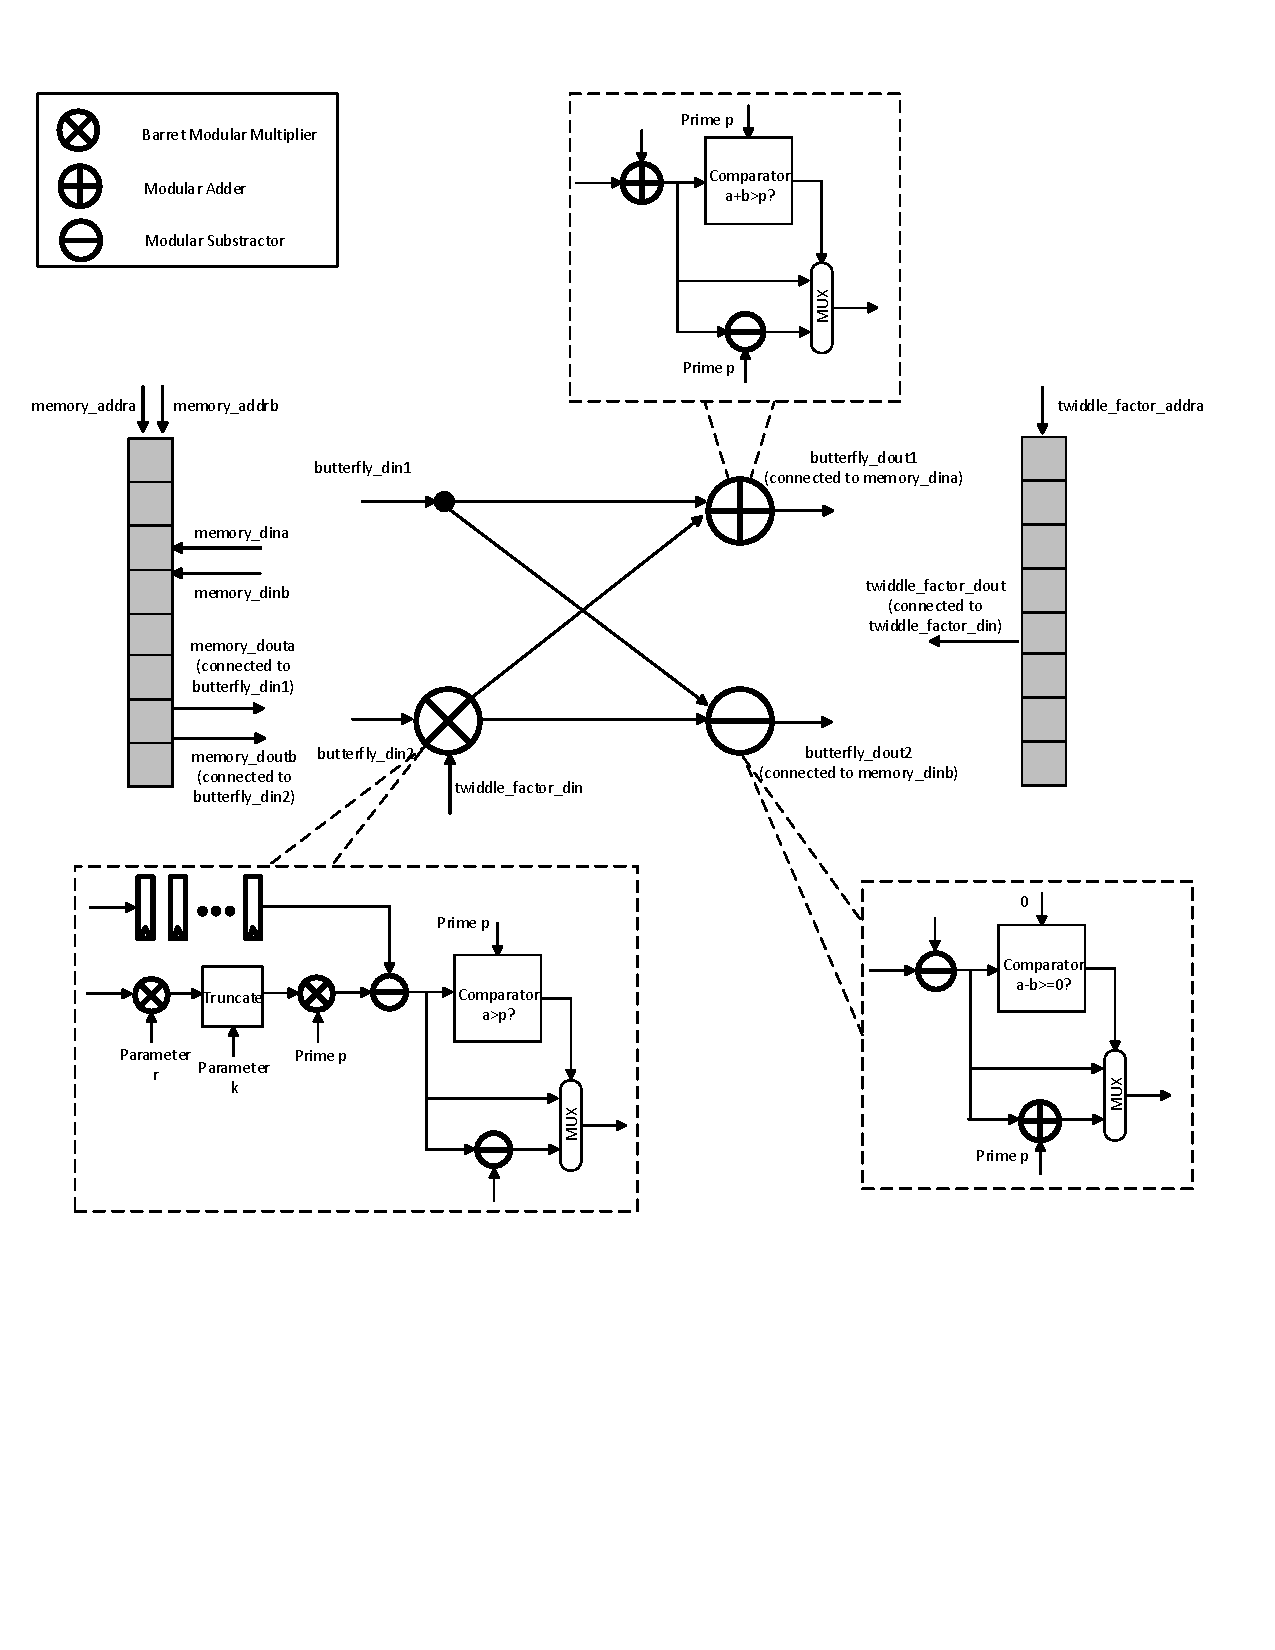
\includegraphics[width=\textwidth]{./fig/processor.pdf}
\caption{Internal structure of butterfly processor}\label{fig:butterfly_processor}
\end{figure*}


\textbf{Design Overview} To perform the butterfly computations and related memory access in each processor efficiently as illustrated in Fig.~\ref{fig:dataswap_with_perm}, a butterfly processor architecture is proposed. Fig.~\ref{fig:butterfly_processor} depicts the internal structure of the butterfly processor. Two memory blocks are instantiated: one dual-port RAM for the $\frac{N}{d}$ points,
and one single-port ROM for the precomputed twiddle factors. At first, two points, \textit{e.g.,} $a_i$ and $a_j$ are simultaneously extracted on \texttt{memory\_douta} and \texttt{memory\_doutb} from the dual-port RAM. Then $a_i$ and $a_j$ are fed to the input ports \texttt{butterfly\_din1} and \texttt{butterfly\_din2} of the butterfly structure. This butterfly structure consists of one Barret modular multiplier (apply Alg.~\ref{alg:modmul}), one modular adder (apply Alg.~\ref{alg:modadd}), and one modular subtractor (apply Alg.~\ref{alg:modsub}). After the butterfly computation is completed, the results $a_i+a_j\cdot w$ and $a_i-a_j\cdot w$ appear at the output ports \texttt{butterfly\_dout1} and \texttt{butterfly\_dout2}. Finally, the two results are simultaneously written back to the RAM through the ports $\texttt{memory\_dina}$ and $\texttt{memory\_dinb}$. It is worth mentioning that
the butterfly processor is fully pipelined such that a pair of valid data \texttt{butterfly\_dout1} and \texttt{butterfly\_dout2} is written back to the RAM every clock cycle, which maintains a relatively high throughput of butterfly computation. This characteristic is crucial for high speed implementation of FHE scheme since the parameter $N$ (the number of NTT points) is typically set to be large for maintaining the hardness of the (Ring-) LWE problem.  


\begin{algorithm}[!tbh]
 \DontPrintSemicolon % Some LaTeX compilers require you to use \dontprintsemicolon instead
 \KwIn{two integers $a$ and $b$ over $\mathbb{Z}_q$}
 \KwOut{ $a\cdot b\in \mathbb{Z}_q$}
    Precompute an integer $k=\lceil log_2q\rceil$\;
    Precompute an integer $r=\lfloor \frac{4^k}{q}\rfloor$\;
    Calculate $x=a\cdot b$\;
    Calculate $t = x - \lfloor\frac{xr}{4^k}\rfloor\cdot q$\;
    \uIf{$t<q$}{
        \Return {$t$\;}
    } \Else{
        \Return{$t-q$\;}
    }
    
 \caption{Barret-Reduction based Modular Multiplication}\label{alg:modmul}
\end{algorithm}

\begin{algorithm}[!tbh]
 \DontPrintSemicolon % Some LaTeX compilers require you to use \dontprintsemicolon instead
 \KwIn{two integers $a$ and $b$ over $\mathbb{Z}_q$}
 \KwOut{ $a+b\in \mathbb{Z}_q$}
    Calculate $t=a+b$\;
    \uIf{$t<q$}{
        \Return {$t$\;}
    } \Else{
        \Return{$t-q$\;}
    }
    
 \caption{Modular Addition}\label{alg:modadd}
\end{algorithm}

\begin{algorithm}[!tbh]
 \DontPrintSemicolon % Some LaTeX compilers require you to use \dontprintsemicolon instead
 \KwIn{two integers $a$ and $b$ over $\mathbb{Z}_q$}
 \KwOut{ $a-b\in \mathbb{Z}_q$}
    Calculate $t=a-b$\;
    \uIf{$t\geq 0$}{
        \Return {$t$\;}
    } \Else{
        \Return{$t+q$\;}
    }
    
 \caption{Modular Subtraction}\label{alg:modsub}
\end{algorithm}

\textbf{Timing analysis} Let  unit one denote the delay of one clock cycle, $T_{mul}$ denote the delay of standard integer multiplication, $T_{modmul}$ denote the delay of Barret reduction based modular multiplication algorithm, and $T_{modadd}$($T_{modsub}$) denote the delay of modular addition(subtraction) algorithm. The delay of one butterfly computation is calculated as
\[
    T_{butterfly} = T_{swap}+T_{mul}+T_{modmul}+T_{modadd}
\]
Note that the proposed butterfly processor is fully pipelined and therefore it takes $T_{butterfly}+\frac{N}{2d}-1$ to process $\frac{N}{2d}$ butterfly computations.

\textbf{Fully pipelined computation} The key point for fully pipelined butterfly computation is to streamline the generation of memory address, \textit{i.e.}, \texttt{memory\_addra} and \texttt{memory\_addrb} in Fig.~\ref{fig:butterfly_processor}. Note that the NTT butterfly address generation pattern is rather complicated: it varies distinctly in different butterfly computation round. It is desirable to implement some other simpler patterns and later combine these simple patterns to create the address generation.  In our design, we use five registers, \texttt{cntb}, \texttt{roundi}, \texttt{dist}, \texttt{cnt}, and \texttt{base} to assist the generation of \texttt{memory\_addra} and \texttt{memory\_addrb} in every clock cycle:

\begin{itemize}
    \item \texttt{cntb}: base counter register, used to generate the basic logic pattern
    \item \texttt{roundi}: butterfly round register, used to indicate the current round of butterfly computation
    \item \texttt{dist}: distance register, used to record the distance between \texttt{memory\_addra} and \texttt{memory\_addrb}
    \item \texttt{cnt}: counter register, used to indicate the incremental offset value for generating \texttt{memory\_addra}
    \item \texttt{base}: the (basis) starting address for \texttt{memory\_addra} in each round of butterfly calculation
\end{itemize}

Moreover, we use two pre-computed arrays $\vec{blk}$ and $\vec{dist}$ to help generate the correct values in the five registers mentioned above. $\vec{blk}$ indicates the number of butterfly blocks in every round of butterfly calculation and has $log_2N$ elements; $\vec{blk}$ indicates the distance between \texttt{memory\_addra} and \texttt{memory\_addrb} in every round of butterfly calculation and has $log_2N$ elements. The construction $\mathbf{blk}$ goes like this: The first $logd$ elements are always $1$; starting from the $(logd+1)$-th element down to the last one, \textit{i.e.} the last $logN-logd$ elements formulate a geometric sequence with initial value $1$ and common ratio $2$. The construction $\mathbf{dist}$ goes like this: The first $logd$ elements are always $\frac{N}{2d}$; Then the last $logN-logd$ elements formulate a geometric sequence with initial value $\frac{N}{2d}$ and common ratio $\frac{1}{2}$.
For example, if $N=32, d=4$, then $\mathbf{blk}=\{1,1,1,2,4\}$ and $\mathbf{dist}=\{4,4,4,2,1\}$.


The generation of \texttt{memory\_addra} and \texttt{memory\_addrb} in Fig.~\ref{fig:butterfly_processor} is formally described in Alg.~\ref{alg:addrgen}. The generated addresses basically map to the memory location of two butterfly inputs (\texttt{butterfly\_din1} and  \texttt{butterfly\_din2} shown in Fig.~\ref{fig:butterfly_processor}). A more concrete example for when $N=32,d=4$ is depicted in Fig.~\ref{fig:timing_diag}. Every register including \texttt{cntb}, \texttt{roundi}, \texttt{dist}, \texttt{cnt}, and \texttt{base} has 5 phases each of which corresponds to one of the $logN=5$ rounds of butterfly computation. Each phase costs 4 clock cycles. For example, \texttt{cntb} updates as $0,1,2,3$ in every phase; whereas \texttt{roundi} updates as $i$ in phase-$i(i=0,1,2,3,4)$. We also assume the calculation of memory address (step6-step7 in Alg.~\ref{alg:addrgen}) takes one clock cycle delay and thus the data appearing in \texttt{memory\_addra} and \texttt{memory\_addrb} is delayed by one clock cycle as shown in Fig.~\ref{fig:timing_diag}. The sequence of \texttt{memory\_addra} and \texttt{memory\_addrb} can be interpreted as follows: In the first clock cycle of phase-0, \texttt{memory\_addra} outputs $0$ and \texttt{memory\_addrb} output $4$ (extracting a[0] and a[4]); in the second clock cycle, \texttt{memory\_addra} outputs $1$ and \texttt{memory\_addrb} outputs $5$, and so on so forth. Finally, in the first clock cycle of phase-4, \texttt{memory\_addra} outputs $0$ and \texttt{memory\_addrb} outputs $1$; in the second clock cycle, \texttt{memory\_addra} outputs $2$ and \texttt{memory\_addrb} outputs $3$, and so on so forth. 


Based on the memory address generation pattern described in Fig.~\ref{fig:timing_diag}, we can finally introduce the complete memory address control logic (See Fig.~\ref{fig:timing_diag2}) used in the proposed butterfly processor. Again, all registers are represented in 5 phases. The register \texttt{current\_state} indicates the current status in each phase:
\begin{itemize}
    \item \texttt{ADDR\_RD}: In this state, butterfly processor reads the corresponding butterfly inputs (\texttt{butterfly\_din1} and \texttt{butterfly\_din2} in Fig.~\ref{fig:butterfly_processor}) from memory in a pipelined fashion
    \item \texttt{IDLE}: This state is optional, and is used only if N is relatively small. For more details, refer to the next section.
    \item \texttt{ADDR\_WR}: In this state, butterfly processor writes back the computed results (\texttt{butterfly\_dout1} and \texttt{butterfly\_dout2} in Fig.~\ref{fig:butterfly_processor}) to memory in a pipelined fashion.
\end{itemize}

Note that the entire butterfly computation takes $logN=5$ iterations. If $N$ is relatively small, the state register transits by $\texttt{ADDR\_RD}\to \texttt{IDLE}\to \texttt{ADDR\_WR}$ in each iteration; otherwise, the state register transits by $\texttt{ADDR\_RD}\to \texttt{ADDR\_WR}$.

In state \texttt{IDLE}, the address is invalid since the purpose of \texttt{IDLE} is to wait for the correct results from the butterfly computing module and thus does not need the address signal to interact with memory. The address pattern used in state \texttt{ADDR\_RD} is identical to that used in \texttt{ADDR\_WR}: our butterfly processor is fully pipelined and, therefore, whenever it reads some data from some specific address in state \texttt{ADDR\_RD}, it must write back to the same location later in state \texttt{ADDR\_WR}.

\begin{algorithm}[!tbh]
 \DontPrintSemicolon % Some LaTeX compilers require you to use \dontprintsemicolon instead
 \KwIn{the number of NTT points $N$ and the number of butterfly processors $d$}
 \KwOut{memory address \texttt{memory\_addra} and \texttt{memory\_addrb} for butterfly computation}
    Precompute $\vec{blk}$ and $\vec{dist}$\;
    \For{$i\leftarrow 0$ \KwTo $logN-1$}{
        \For{$blk\leftarrow 0$ \KwTo $blk[i]-1$}{
            \texttt{base}  $\leftarrow\frac{N}{d\cdot blk[i]}\cdot blk$\;
            \For{$cnt\leftarrow 0$ \KwTo $\frac{N}{2d\cdot blk[i]}-1$}{
                \texttt{memory\_addra} $\leftarrow base + cnt$\;
                \texttt{memory\_addrb} $\leftarrow base + cnt + dist[i]$\;
            }
        }
    } 
    
 \caption{Memory address generation for butterfly computation}\label{alg:addrgen}
\end{algorithm}


\begin{figure*}[!tb]
\centering
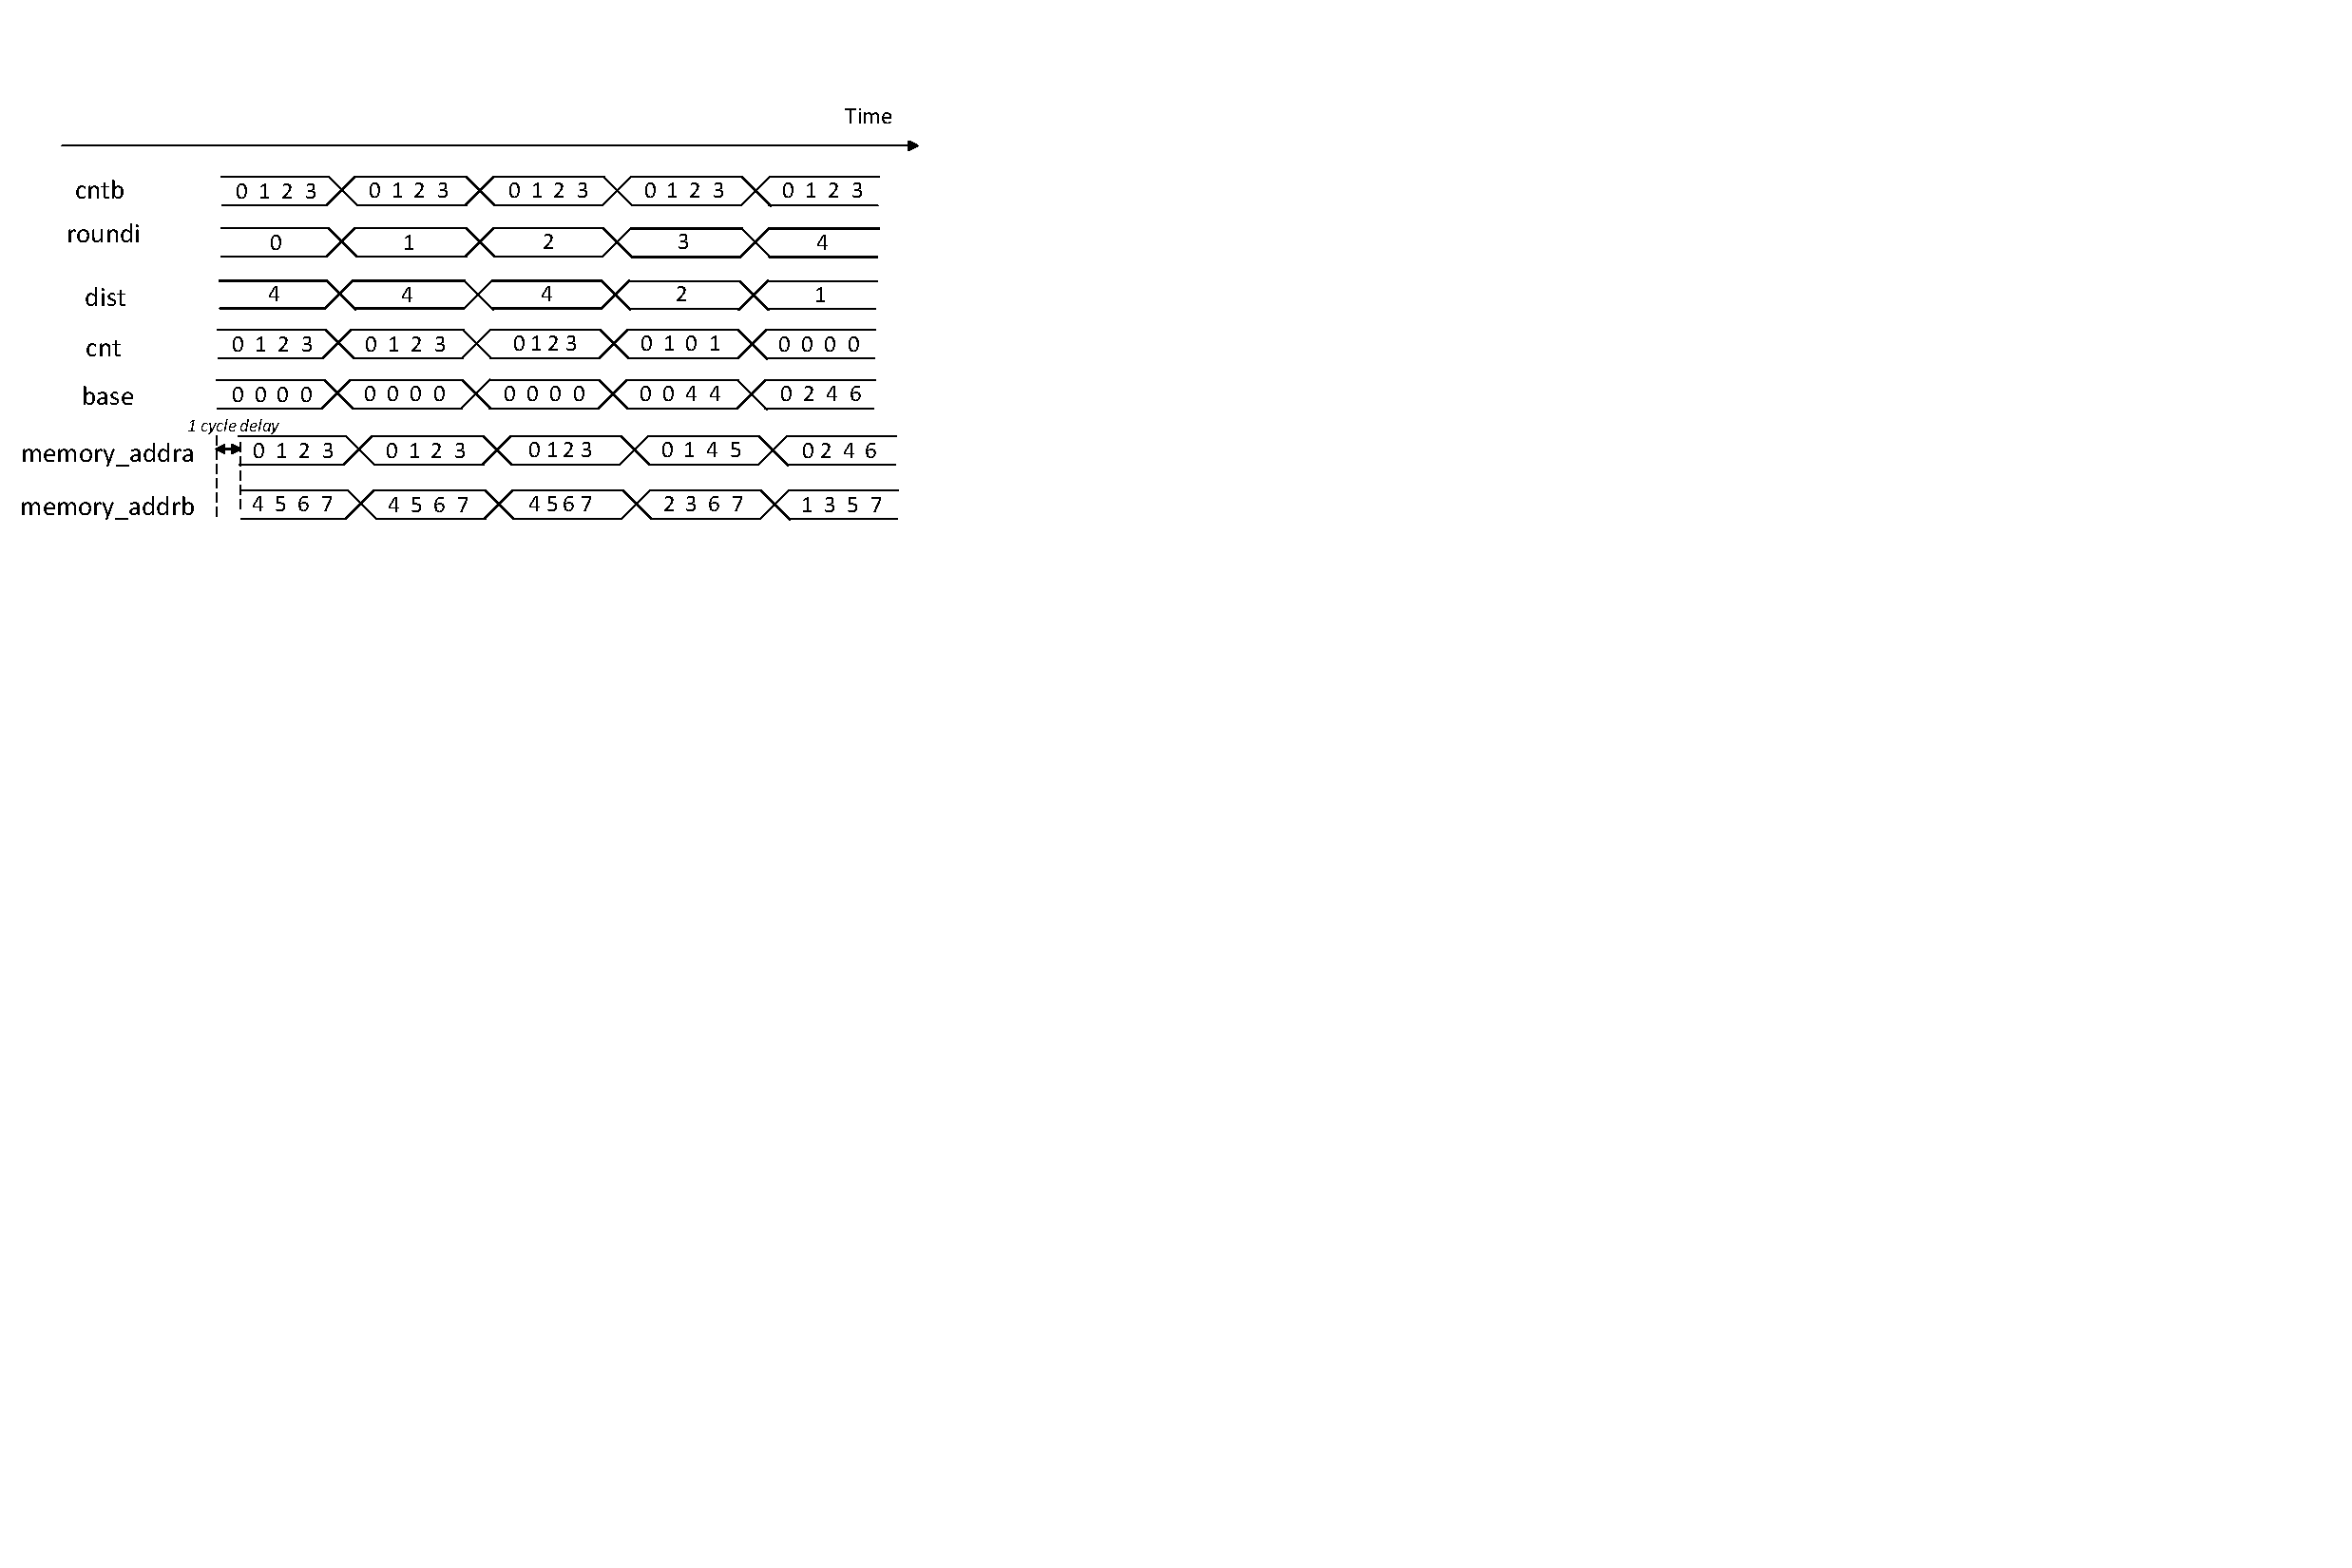
\includegraphics[width=\textwidth]{./fig/timing_diag.pdf}
\caption{Illustrative timing diagram for memory address generation in line with Alg.~\ref{alg:addrgen}($N=32, d=4$)}\label{fig:timing_diag}
\end{figure*}

\begin{figure*}[!tb]
\centering
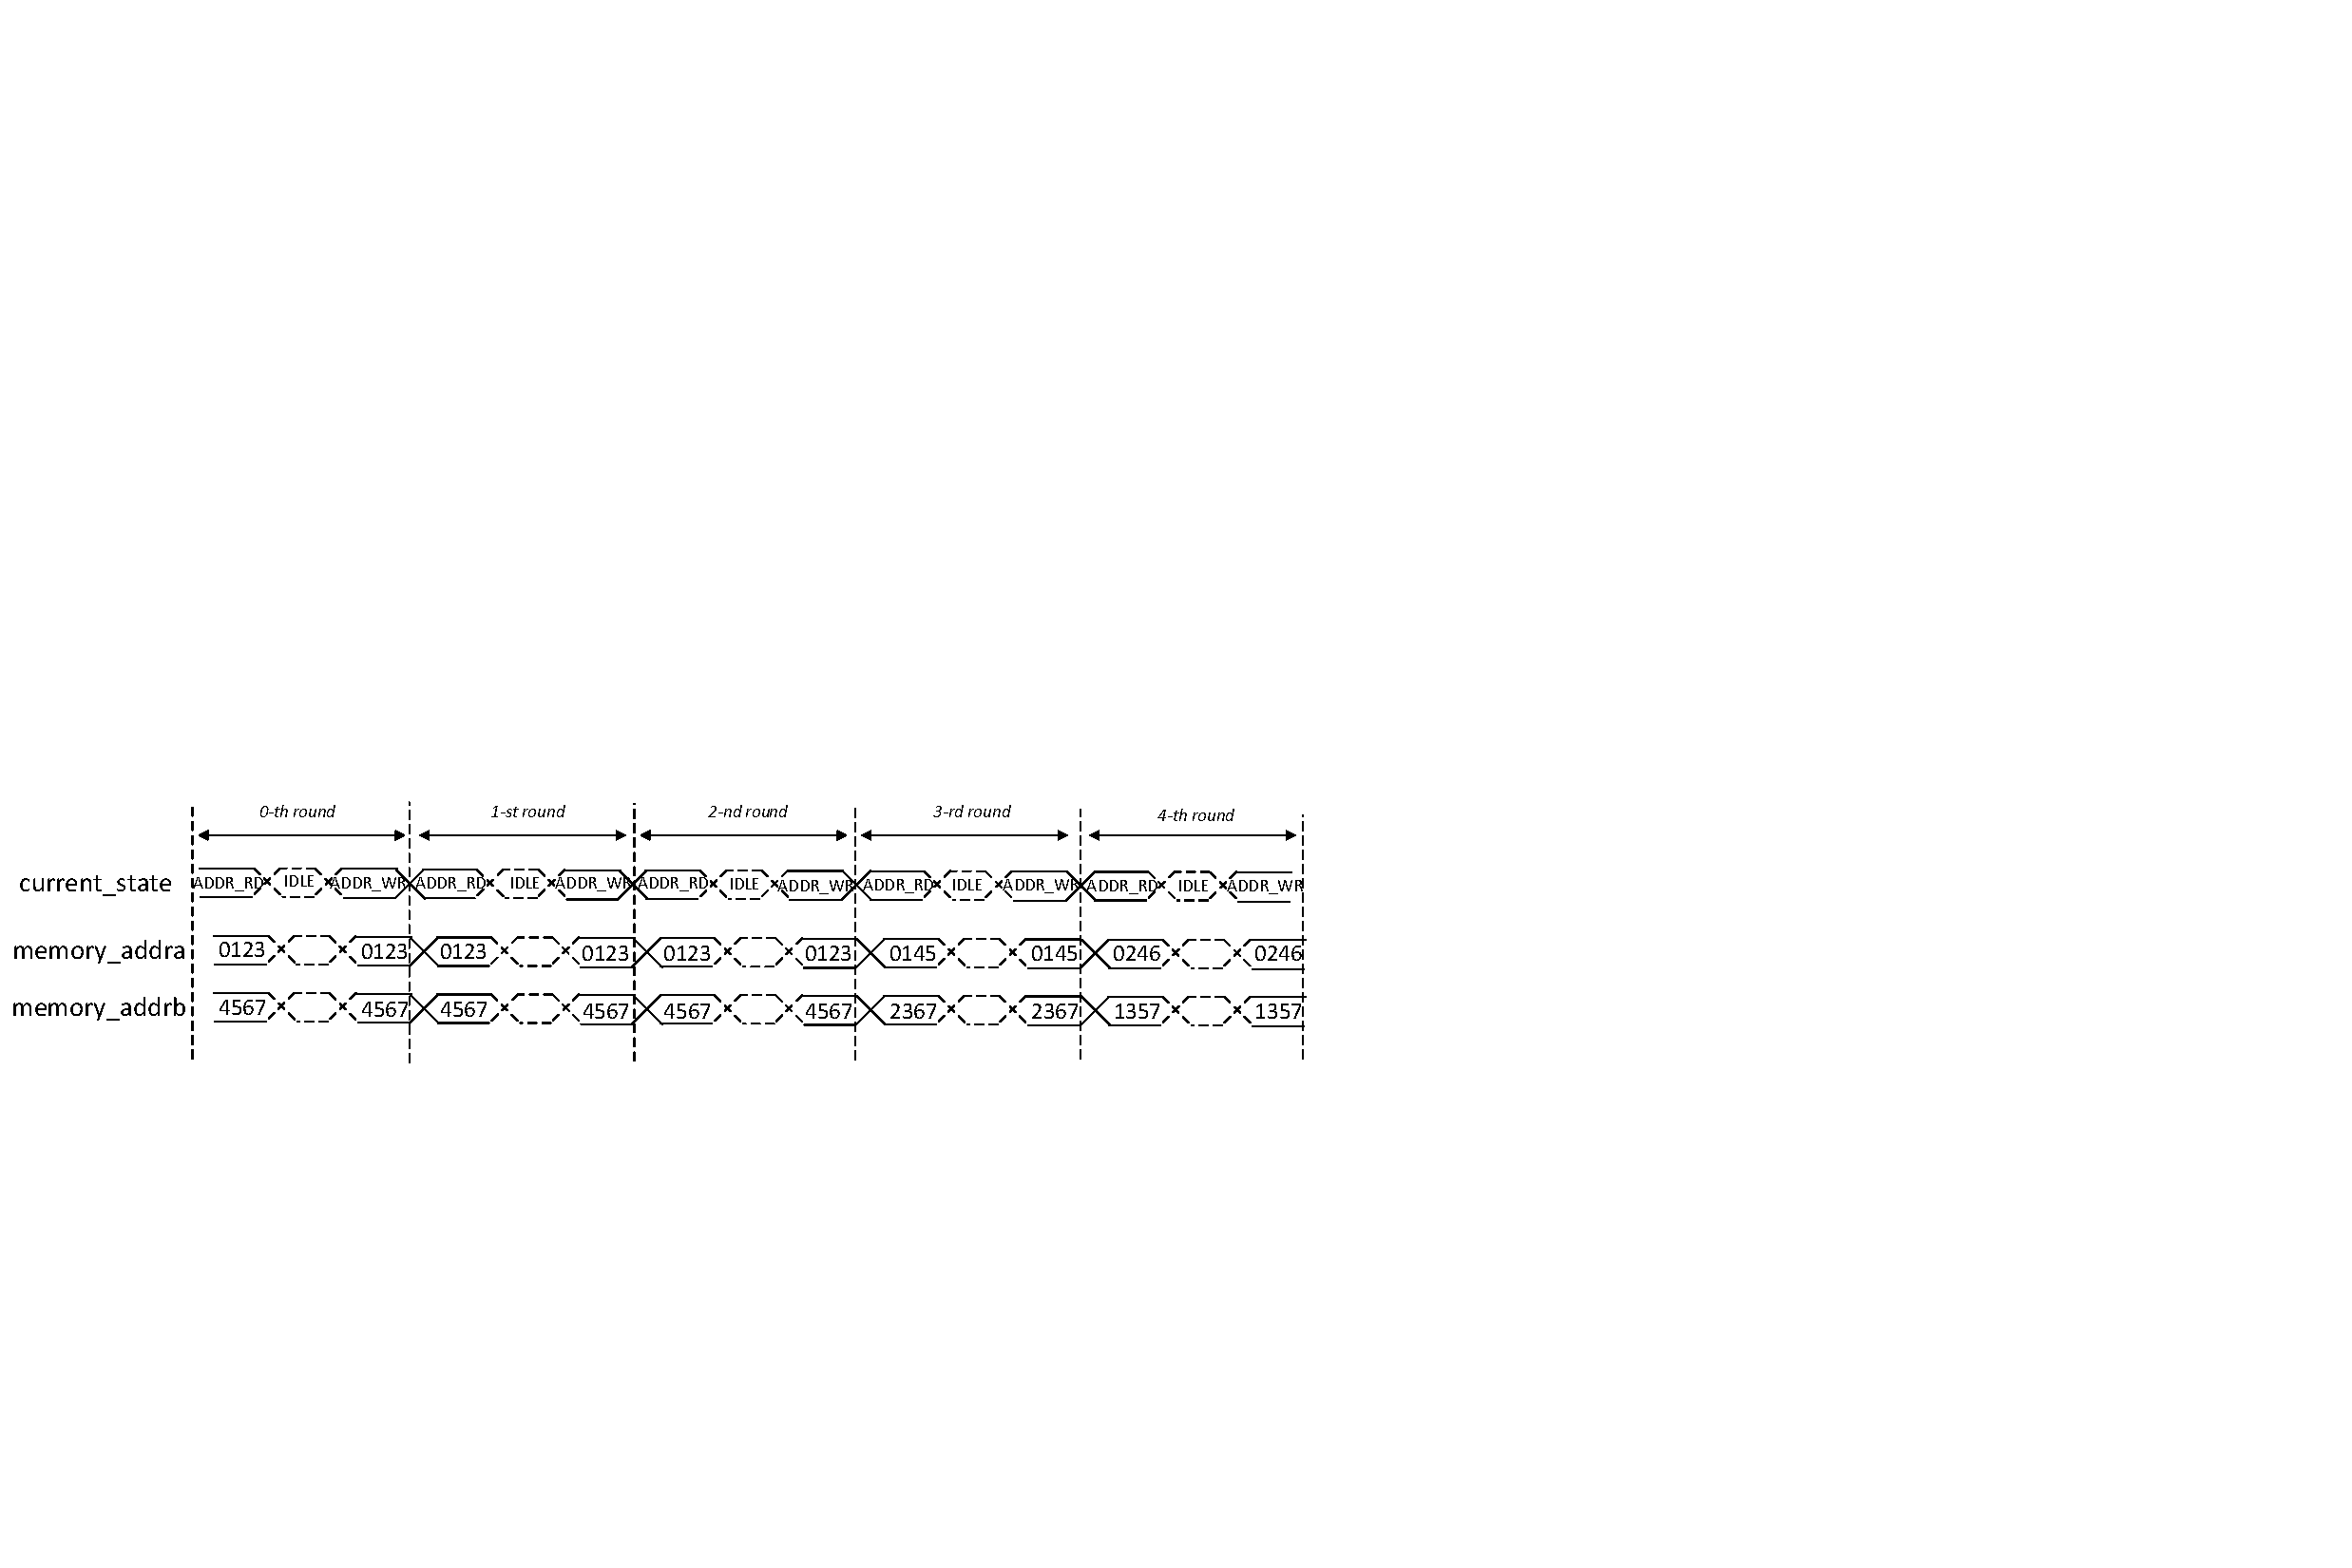
\includegraphics[width=\textwidth]{./fig/timing_diag2.pdf}
\caption{Top-level timing diagram for hypercube NTT in 5 rounds($N=32, d=4$)}\label{fig:timing_diag2}
\end{figure*}


\subsection{Implementation Experiments}
Finally, we test the performance of our systolic array for Gaussian elimination in compliance with ROLLO-II.encrypt. The implementation results are collected in Table~\ref{table:hypercube-ntt-result}.
 
 \begin{table*}[!t]\centering
 \caption{Performance of the configurable hypercube NTT hardware for FHEW-like FHE schemes on Xilinx Artix-7 FPGA}
 \label{table:hypercube-ntt-result}
 \begin{minipage}{\textwidth}\centering
 \scalebox{0.8}{\begin{tabular}{lcccccc}
 \hline
 Instance   & \# of processors & freq & cycle & CLB/LUT/Reg &   memory & DSPs \\
 \hline
 \multirow{5}{*}{$N=1024,q\approx 2^{32}$} & 2 & 100 & 5120 & 451/2309/1756  & 3 & 30 \\
             &                                        4 & 100 & 2560 & 760/3581/2940 &   6 & 60 \\
             &                                        8 & {100} & 1280  & 1402/4238/5480 & 12  & 120 \\
             &                                        16 & 100 & 640 & 2174/10669/10591 & 24 & 240 \\
             &                                        32 & 100 & 430 & 3937/19250/18738 & 48 & 480 \\
             &                                        64 & 80 & 350 & 7835/39009/37060 & 96 & 960 \\
 \hline
  \hline
 \end{tabular}}
 \end{minipage}
 \vspace{0mm}
 \end{table*}


\textbf{Timing analysis} The main states we used are \texttt{MEM\_READ} and \texttt{MEM\_WRITE}. If the delay of butterfly computation is longer than that of \texttt{MEM\_READ}, then an auxillary state called \texttt{IDLE} is inserted in between. Precisely speaking, if $\frac{N}{2d}-T_{mem\_read}+1<T_{butterfly}$, then \texttt{IDLE} with delay $T_{IDLE}=T_{butterfly}-\frac{N}{2d}+T_{mem\_read}-1$ is required. The delay for the state \texttt{MEM\_READ} and the state \texttt{MEM\_WRITE} are $\frac{N}{2d}$ respectively. In summary, the total delay for the hypercube NTT with $d$ processors is:
\[
    logN\cdot\left(\frac{N}{d}+max(T_{IDLE},0)\right )
\]

In our concrete experiment, $T_{mem\_read}$ set to $1$ and $T_{butterfly}$ set to $27$. Therefore the total delay for the hypercube NTT is further simplified to $logN\cdot(\frac{N}{d}+max(27-\frac{N}{2d},0))$.


\textbf{Experimental data} The proposed design is implemented on Xilinx Zynq UltraScale+ ZCU106 evaluation board using Vivado 2018.1. The number of NTT points is set to 1024, a typical value used in FHE schemes. The number of NTT processors is configured to 2,4,8,16,32, and 64 to fully demonstrate the scalability of our hypercube NTT design. It is worth mentioning that our implementation follows the parameterized design approach, \textit{i.e.}, our NTT hardware can be customized and auto-generated on the fly from a script file by inputting core parameters of hypercube NTT, for example, $N$ and $d$. The experimental results are collected in Table.~\ref{table:hypercube-ntt-result}. As the parameter $d$ increases, the clock frequency is rather stable around $100$ MHz, which indicates the hypercube memory swapping strategy is successful to maintain a good critical path delay. 
If the number of processors is smaller than $32$, the cycle delay equals to $logN\cdot\frac{N}{d}$ and thus the increase of $d$ reduces significantly the cycle delay: for example, doubling $d$ suggests cycle delay reduced by half. As the number of processors gets even bigger ($\geq 32$), the \texttt{IDLE} state is inserted and the cycle delay equals to $logN\cdot(\frac{N}{2d}+27)$ for which the performance boost by increasing $d$ is rather marginal.  For this case, we can optimize the performance of butterfly computation (more concretely, modular reduction) to further improve it. However, we do not push the limit on this direction which is not the focus in this paper.

\section{System Integration on Xilinx MPSOC platform}
This section describes the ROLLO hardware at a higher level. It is worth mentioning that the CPA-secure ROLLO can be converted to a CCA2-secure KEM when the HHK \cite{hofheinz2017modular} framework for the Fujisaki-Okamoto transformation is applied. Therefore, we focus on the CCA2-secure parameter sets and include the core functionalities, \textit{e.g.}, encryption and decryption in this work. Firstly, the ROLLO encryption hardware, together with its key components, is presented, evaluated, and compared with related work; Then the ROLLO decryption hardware is presented, evaluated, and compared. In particular, the Rank Support Recovery algorithm which is the kernel of the decoding of LRPC codes is optimized and further adapted for efficient hardware implementation.



\textbf{Performance}
The cycle count information for the proposed ROLLO decryption hardware on Artix-7 is collected in Table~\ref{table:rollo-decrypt}. The primary factor accountable for the cycle delay is the RSR algorithm which relies on the Gaussian elimination systolic array; The secondary factor is the $\mathbb{F}_{2^m}[z]$ multiplication.
Note that the performance of ROLLO-II decryption is about 2-3 times worse than that of ROLLO-I. This observation can be interpreted as follows: The primary and the second factors are more or less a quadratic function of
$n$ and $m$ as $n^2+m\cdot n$. The value of $n$ used in ROLLO-II is about twice as large as ROLLO-I and this gives rise to the overall 2-3 times of performance degradation.

\begin{table*}[!t]\centering
 \caption{Detailed cycle count analysis on ROLLO decryption/decapsulation for the claimed 128-bit/192-bit/256-bit security level (SL), respectively}
 \label{table:rollo-decrypt}
 \begin{minipage}{\textwidth}\centering
 \scalebox{1}{\begin{tabular}{llcc}
 \hline
 Process & & ROLLO-I.decap& ROLLO-II.decrypt  \\
 \hline
\multirow{3}{*}{generate K } &\multirow{1}{*}{compute $\mathbf{s}$}  & 2452/2984/5018 & 12544/14122/17806  \\
 &\multirow{1}{*}{generate $\mathbf{S_i}$}  & 6024/7032/11241 & 15168/17032/20943   \\
 &\multirow{1}{*}{$\mathbf{E}\gets RSR(\cdot)$}  & 16231/22881/36174 & 41736/48717/59931   \\
 &\multirow{1}{*}{SHA3}  & 189/216/243 & 189/216/216   \\
\hline
Total & --- & 24,896/33,113/52,676 & 69,637/80,087/98,896\\
\hline
 \end{tabular}}
 \end{minipage}
 \vspace{-4mm}
 \end{table*}

Compared with the optimized software implementation using AVX2 instructions included in the ROLLO NIST submission, the cycle count is reduced by at least 20 and 16 times for ROLLO-I, and ROLLO-II, respectively;
% \begin{table*}[!t]\centering
% \caption{Implementation results for ROLLO decryption compared with other PQC candidates on Xilinx Artix-7 FPGA}
% \label{table:rollo-encrypt-fpga}
% \begin{minipage}{\textwidth}\centering
% \scalebox{1}{\begin{tabular}{lcccccccc}
% \hline
% Instance  & \tabincell{c}{freq\\(MHz)} & \tabincell{c}{time\\($\mu$s)} & cycle & slice & LUT & reg & RAM & slice*cycle/freq\\
% \hline
% \multirow{1}{*}{ROLLO-I-128-decap} & 180 & 34& 6,184 & 8577 & 28056 & 14432 & 24.5 & $2.95\times 10^5$\\
% \multirow{1}{*}{ROLLO-I-192-decap} & 180 & 38& 6,851 & 13366 & 43458 & 19904 & 32.5 & $5.09\times 10^5$\\
% \multirow{1}{*}{ROLLO-I-256-decap} & 180 & 60& 10,793 & 13496 & 44511 & 23036 & 35.5 & $8.09\times 10^5$\\
%  \hline
% \multirow{1}{*}{ROLLO-II-128-decrypt} & 175 & 177& 30,929 & 9769 & 32105 & 15601 & 29 & $1.73\times 10^6$\\
% \multirow{1}{*}{ROLLO-II-192-decrypt} & 175 & 184& 32,166 & 12624 & 39307 & 20591 & 36 & $2.32\times 10^6$\\
% \multirow{1}{*}{ROLLO-II-256-decrypt} & 175 & 198& 34,673 & 15456 & 48461 & 25600 & 43.5 & $3.06\times 10^6$\\
%  \hline
% \multirow{1}{*}{ROLLO-III-128-decap} & 160 & 41& 6,483 & 15195 & 48029 & 23140 & 45.5 & $6.16\times 10^5$\\
% \multirow{1}{*}{ROLLO-III-192-decap} & 140 &57& 7,944 & 13887 & 45368 & 23473 & 40.5 & $7.88\times 10^5$\\
% \multirow{1}{*}{ROLLO-III-256-decap} & 120 &91& 10,958 & 14091 & 46755 & 24262 & 40.5 & $1.29\times 10^6$\\
% \hline
% \end{tabular}}
% \end{minipage}
% \vspace{-4mm}
% \end{table*}
Compared with other PQC hardware implementations on FPGA listed in Table.~\ref{table:dec_compare}, the decryption throughput of ROLLO is advantageous: It is apparently faster than the quasi-cyclic MDPC/LDPC code based schemes including BIKE \cite{richter2020folding} and LEDAkem \cite{hu2019lightweight}, and even approaches the state-of-art implementation of the Niederreiter cryptosystem featuring high speed \cite{wang2018fpga}; BIKE and LEDAkem appear to outperform ROLLO and Classic McEliece in terms of slices and BRAM usage. On the other hand, ROLLO uses fewer slices and BRAMs but runs slower than the Classic McEliece~\cite{bernstein2020classic} which measures the core mathematical functions not including, \textit{e.g.}, hashing at the same security level. It is worth mentioning that our design targets embedded systems with limited resources, and the footprint persists as the parameters escalates, which can be tolerated on low-cost Artix-7 FPGAs.

\begin{table*}[t]
\centering
\begin{minipage}{1\textwidth}\centering
\caption{Performance of ROLLO-I/II decryption hardware and comparison with existing work on
PQC hardware, targeting NIST security levels $1/3/5$. All the designs are synthesized on an Artix-7 FPGA.}
\label{table:dec_compare}
 \scalebox{.75}{\begin{tabular}{lcccccccc}
\hline
Scheme &\tabincell{c}{SL [bits]}&Platform &$f_{\text{max}}$[MHz] & Time/Op & Cycles  & Slices/LUTs/FFs & BRAM\\
\hline
LRPC code:\\
\textbf{ROLLO-I-128} & \multirow{2}{*}{128} & \multirow{2}{*}{Artix-7} & 180  & 138$\mu s$ & $2.49\times 10^4$ & 11412/36772/21832 & 23.5\\
\textbf{ROLLO-II-128} &                    &                         & 175  & 398$\mu s$ & $6.96\times 10^4$ &14160/45207/26598 & 29\\
\hdashline
\textbf{ROLLO-I-192} & \multirow{2}{*}{192} & \multirow{2}{*}{Artix-7} & 180  & 184$\mu s$ & $3.31\times 10^4$ & 12724/40465/25079 & 26.5\\
\textbf{ROLLO-II-192} &                   &                           &175 & 458$\mu s$ & $8.01\times 10^4$ & 15357/49855/30831 & 33\\
\hdashline
\textbf{ROLLO-I-256} & \multirow{2}{*}{256} & \multirow{2}{*}{Artix-7}   & 180 & 293$\mu s$ & $5.27\times 10^4$ & 15130/49419/30623 & 34.5\\
\textbf{ROLLO-II-256} &                  &                          &175 & 565$\mu s$ & $9.89\times 10^4$ & 15620/51852/30641 & 34.5\\
\hline
 MDPC/LDPC code:\\
pre-BIKE\cite{heyse2013smaller} & {80} & {Virtex-6} & {222.5}  & $125.38\mu s$& $2.79\times 10^4$  & 2920/8856/14426 & 0\\
BIKE\cite{richter2020folding} & {128} & {Artix-7} & {100}  & $1.90 ms$& $1.90\times 10^5$  & 8862/30977/5092 & 29\\
BIKE\cite{richter2020folding} & {256} & {Artix-7} & {100}  & $6.11 ms$& $6.11\times 10^5$  & 8997/30772/5096 & 30\\
LEDAkem\cite{hu2019lightweight} & 128 & Artix-7 & 140  & $18.7 ms$& $2.62\times 10^6$  & 870/2222/658 & 13\\
\hline
Goppa code:\\
Niederreiter\cite{wang2018fpga} &{128} &{Virtex-6} & {267}   & $40 \mu s$    & $1.02\times 10^4$  & 6571/---/---& 23\\
Classic McEliece\cite{bernstein2020classic} &{128} &{Artix-7} & {105.6}   & $95 \mu s$    & $10^4$  & {---/81339/132190}& {236}\\
Classic McEliece\cite{bernstein2020classic} &{192} &{Virtex-7} & {130.8}   & $112 \mu s$    & $1.46\times 10^4$  & {---/109484/168939}& {446}\\
Classic McEliece\cite{bernstein2020classic} &{256} &{Virtex-7} & {136.6}   & $181 \mu s$    & $2.47\times 10^4$  & {---/122624/186194}& {589}\\
\hline
\end{tabular}}
\end{minipage}
\end{table*}

\section{Conclusions}
This paper presented a complete FPGA implementation of the ROLLO scheme using LRPC codes.
It is the first hardware implementation of a rank-metric code based cryptosystem that supports varying security parameters. The efficiency of our design is achieved by a novel Gaussian elimination structure, a simplified implementation strategy for the rank support recovery algorithm, and a fast interleaved polynomial multiplier, among others. The proposed parameterized architectures, such as the Gaussian elimination and the polynomial multiplication, are not limited to instances used in ROLLO but also fully support other rank-code based schemes. For example, RQC applies the identical family of ideal codes to construct the public key and the ciphertext, therefore, the $\mathbb{F}_{2m}[z]$ arithmetic presented in this work can be directly reused as the underlying arithmetic; At the core of RQC key generation and data encryption algorithm, the generation of vectors over $\mathbb{F}_{2}$ with prescribed rank weight is demanding, and the parameterized Gaussian elimination systolic array can be adpated effortlessly for this task.

\bibliographystyle{alpha}
\bibliography{./reference}
\end{document}
